\documentclass[manuscript,screen,review]{acmart}

\usepackage{algorithm}
% Use algorithmicx + algpseudocode: provides \Require, \Ensure, \State, and \Comment
\usepackage{algorithmicx}
\usepackage{algpseudocode}
\usepackage{tikz}
% Load common tikz libraries used in figures (positioning provides the "of" syntax)
\usetikzlibrary{positioning,arrows.meta,calc,shapes,shadows}
% color support for \textcolor used inside algorithms
\usepackage{xcolor}
% Math packages required for \text and bold symbols inside math
\usepackage{amsmath}
\usepackage{bm}
\usepackage{multirow}
% Enable list customization (leftmargin, itemsep, etc.) used in the document
\usepackage{enumitem}
% Ensure header height is sufficient for fancyhdr
\setlength{\headheight}{20.48303pt}
% Visible placeholder for numbers still awaiting the controlled matrix run.
% Every occurrence must be gone before submission: grep for \TBD.
\newcommand{\TBD}[1]{\textcolor{red}{\textbf{[TBD:} #1\textbf{]}}}
% theorem environments used in the document
\usepackage{amsthm}
\newtheorem{assumption}{Assumption}
\newtheorem{problem}{Problem}
% Define remark environment (was missing and caused compilation errors)
\newtheorem{remark}{Remark}
% Source environment names stay prop / lem; printed labels are English.
\newtheorem{prop}{Proposition}
\newtheorem{lem}{Lemma}

\renewcommand{\figurename}{Figure}
\renewcommand{\tablename}{Table}
\floatname{algorithm}{Algorithm}
\renewcommand{\proofname}{Proof}

%% ===================== Rebuild order for figures and tables =====================
%% Sequential. Steps 1--2 run in clbs/; steps 3--4 at the repository root.
%%
%%  1. Main result (~6 h; every headline number below comes from this):
%%       py -u -m tools.baseline_ladder --budget 90 \
%%          --seeds 42,7,2024,13,1,99,123,777,31415,8      -> output/baseline_ladder.csv
%%  2. Three companion batches (after 1; no dependence among themselves):
%%       py -u -m tools.prune_ablation --budget 90         -> output/prune_ablation.csv
%%       py -u -m tools.ladder_diag  --budget 90           -> output/ladder_cost.csv
%%                                                            output/ladder_convergence.csv
%%                                                            output/case_study/*.json
%%     Do not run these in parallel with step 1: all use a wall-clock budget and
%%     would steal evaluations from each other, which breaks the equal-wall-clock
%%     protocol of Section 5.1.
%%  3. Tables and macros (seconds):
%%       py paper01/tab/gen_tables_ladder.py
%%     Writes tab/*.tex (Chinese paper) and tab/*_EN.tex (this file), and prints
%%     the macro block below for pasting. Tables and macros share one source.
%%  4. Figures (seconds; needs matplotlib):
%%       py paper01/fig/render_all.py         (skip a figure if its data is missing)
%%     This manuscript includes the English PDFs (no _CN suffix).
%%     CLBS_FIG_PNG=1 also writes png previews.
%%  5. Self-check (seconds; no TeX engine):
%%       py paper01/check_tex.py paper01/paper_EN.tex
%%     Undefined macros, hard-coded numbers, brace/environment pairing,
%%     dangling cross-refs, leftover TODOs.
%%
%% Data completeness (checked 2026-08-16): all nine figures have data on disk.

%% ===================== Single source for headline numbers =====================
%% Prose always cites the macros below; never hard-code a percentage.  Source:
%% clbs/output/baseline_ladder.csv from clbs/tools/baseline_ladder.py
%% (in clbs/: py -u -m tools.baseline_ladder --budget 90 --seeds ...).
%% Convention: 10 instances x 10 seeds = 100 pairs, equal wall-clock budget,
%% paired Wilcoxon signed-rank.  Regenerated by tab/gen_tables_ladder.py.
%%
%% Narrative that must not be reverted to a 4-seed reading:
%%  (1) open-loop dispatching is significant (4.59%, p<1e-4);
%%  (2) end-to-end 21.35% < independent product 22.6% --- near-additive, not a
%%      positive interaction;
%%  (3) B NA/NM 0.5, B0->B1 is negative (closed loop still helps); large-fleet
%%      B cells have B1->B2 positive.  Do not rewrite (3) as an applicability
%%      upper bound --- that claim was withdrawn after the 2026-08-16
%%      per-instance check (see the vehicle-to-arm-ratio block below).
%%
%% tab_bytag uses the same estimator as this block: mean of pairwise relative
%% gains.  The ten-instance mean then equals the pooled macros.  The gain
%% column cannot be recovered by dividing the two means on the same row.
\newcommand{\NCases}{10}
\newcommand{\NSeeds}{10}
\newcommand{\NPairs}{100}
% Closed loop itself (dispatching rule fixed; only whether delay enters search)
\newcommand{\GainLoopRule}{18.86\%}      % B0  -> B1 , rule-based
%% Every P-macro is Holm-adjusted over the five contrasts of tab:main.
%% The correction is inert on those five (largest p has multiplier 1).
%%
%% !! Each P-macro carries its own relation ("<" or "=").  Write $p\PLoopRule$
%% !! with no extra equals.  Wilcoxon reports 0.0000 below 1e-4; "p=0.0000"
%% !! would claim a zero p.  If the relation lived in the body, a re-run that
%% !! pushed a p under the floor would render "p=<10^{-4}".  pmac() in
%% !! gen_tables_ladder.py chooses the relation.
\newcommand{\PLoopRule}{<10^{-4}}
\newcommand{\GainLoopProbe}{17.75\%}     % B0+ -> B2 , reservation-table-aware
\newcommand{\PLoopProbe}{<10^{-4}}
% Reservation-table-aware dispatching (closed-loop factor fixed)
\newcommand{\GainProbeOpen}{4.59\%}      % B0  -> B0+, open-loop, now significant
\newcommand{\PProbeOpen}{<10^{-4}}
\newcommand{\GainProbeLoop}{2.45\%}      % B1  -> B2 , in the closed loop
\newcommand{\PProbeLoop}{=0.0054}
% End-to-end: literature structure -> this paper
\newcommand{\GainEndToEnd}{21.35\%}      % B0  -> B2
\newcommand{\PEndToEnd}{<10^{-4}}
\newcommand{\WinEndToEnd}{94}
\newcommand{\LoseEndToEnd}{5}
%% ---- Effect size: Hodges--Lehmann pseudomedian and 95% CI ----
%% The Gain macros are means of pairwise relative gains and carry no precision;
%% they are a different source from the Wilcoxon p (ranks).  The HL pair is the
%% estimator of that test; interval from stats.py hodges_lehmann_ci
%% (Hollander--Wolfe; n=100 uses the normal approximation).  Both macros are
%% absolute values (a reduction is positive); endpoints are ordered by
%% magnitude.  Only the two contrasts quoted in the prose are supplied.
\newcommand{\HLLoopRule}{18.28\%}
\newcommand{\CILoopRule}{$[14.68\%,\ 21.95\%]$}
\newcommand{\HLProbeLoop}{3.03\%}
\newcommand{\CIProbeLoop}{$[0.94\%,\ 5.19\%]$}
% End-to-end if the two mechanisms were independent.  Observed is slightly lower.
\newcommand{\GainIndepProduct}{22.6\%}
%% How many of the ten instances are significant on their own.  Section 5.5
%% reads signs per instance, i.e. ten tests in a ten-instance family, so the
%% family must be corrected.  Family = the ten instances of one effect (two
%% families, not twenty).  Holm controls FWER; BH agrees (see the generator).
%% Closed loop: 9/10 raw and 9/10 Holm (largest Holm p=0.0401).
%% Dispatching: 2/10 raw (Family C), 0/10 Holm.  Prose uses the Adj counts;
%% raw counts stay so Section 5.5 can state the difference.  Do not revive
%% "Family C is the only family that supports a conclusion" from the raw 2/10.
\newcommand{\CellsSigLoop}{9}
\newcommand{\CellsSigLoopAdj}{9}
\newcommand{\CellsSigProbe}{2}
\newcommand{\CellsSigProbeAdj}{0}
%% ---- Vehicle-to-arm-ratio family (funnel layout), full four-point B1->B2 ----
%% !! None of the four is significant (p = 0.4121 / 0.2011 / 0.1386 / 0.3313),
%% !! and the signs alternate:
%% !!   0.5 -4.67% | 1.0 +5.04% | 1.5 -4.63% (= A funnel) | 2.0 +5.71%
%% !! Do not narrate a fleet-size threshold.  The generator warns if signs
%% !! are not monotone.
%%
%% Per-instance macros carry their own sign (negative = lower makespan = better).
%% Quote them bare.  Pooled Gain macros are absolute; the prose carries direction.
%% \GainProbeStarve is the one exception: the body writes $-\GainProbeStarve$.
\newcommand{\GainLoopStarve}{-2.0\%}     % B NA/NM 0.5, B0->B1 (closed loop n.s.)
\newcommand{\GainProbeStarve}{4.7\%}     % B NA/NM 0.5, B1->B2 (gain direction; n.s.)
\newcommand{\GainProbeFleetBase}{-4.6\%} % A funnel (N_A/N_M=1.5), B1->B2 (n.s.)
\newcommand{\GainProbeFleetOne}{+5.0\%}  % B NA/NM 1.0, B1->B2 (n.s.)
\newcommand{\GainProbeFleetTwo}{+5.7\%}  % B NA/NM 2.0, B1->B2 (n.s.)
%% ---- Remaining per-instance readings quoted in Section 5.5 ----
%% Same cell_gain / cell_p as tab_bytag.  Each carries its own sign.
\newcommand{\GainLoopFunnel}{-21.3\%}    % A funnel , B0->B1
\newcommand{\GainLoopHigh}{-26.6\%}      % A high
\newcommand{\GainLoopMid}{-14.4\%}       % A mid
\newcommand{\GainLoopLow}{-10.3\%}       % A low
\newcommand{\GainLoopScatter}{-8.1\%}    % A scatter
\newcommand{\GainLoopFleetOne}{-15.6\%}  % B NA/NM 1.0
\newcommand{\GainLoopFleetTwo}{-37.7\%}  % B NA/NM 2.0
\newcommand{\GainLoopFlexLo}{-29.7\%}    % C F=0.3
\newcommand{\GainLoopFlexHi}{-22.9\%}    % C F=1.0
\newcommand{\GainProbeFlexLo}{-8.2\%}    % C F=0.3 , B1->B2 (largest of ten)
\newcommand{\GainProbeFlexHi}{-7.2\%}    % C F=1.0 , B1->B2
%% Four fleet p-values are uncorrected on purpose: even raw they miss the threshold.
\newcommand{\PProbeFleetHalfRaw}{=0.4121}
\newcommand{\PProbeFleetOneRaw}{=0.2011}
\newcommand{\PProbeFleetBaseRaw}{=0.1386}
\newcommand{\PProbeFleetTwoRaw}{=0.3313}
%% Flexibility is the only family whose verdict moves under correction.
\newcommand{\PProbeFlexLoRaw}{=0.0105}
\newcommand{\PProbeFlexLoHolm}{=0.1052}
\newcommand{\PProbeFlexLoBH}{=0.1052}
\newcommand{\PProbeFlexHiRaw}{=0.0321}
\newcommand{\PProbeFlexHiHolm}{=0.2885}
\newcommand{\PProbeFlexHiBH}{=0.1603}
%% Largest still-significant closed-loop Holm p: the family's verdict does not
%% hinge on whether a correction is applied.
\newcommand{\PLoopCellMax}{=0.0401}
% Contention-intensity range (min/max of the 10-instance contention column)
\newcommand{\ContentionLo}{6.6\%}
\newcommand{\ContentionHi}{33.5\%}
%% Layout family's own upper end, not the global max (that is C F=1.0, same
%% funnel layout at full flexibility).  Use this macro for the span of Family A
%% (Section 5.1.1 and the introduction).  Abstract generation range and the
%% common-executor optimistic gap stay \ContentionHi (global).
\newcommand{\ContentionAHi}{31.9\%}
%% Evidence that the layout family is spliced: LU-to-farthest-arm unimpeded
%% haul is identical on the three dumbbell cells and identical on the two grid
%% cells.  Section 5.1.1 is therefore "capacity sweep + topology contrast",
%% not "capacity only".  The generator asserts within-segment equality.
%% Do not use the composite LB of tab:instances as a proxy for distance.
\newcommand{\LegDumbbell}{10.0}          % funnel/high/mid, identical
\newcommand{\LegGrid}{18.0}              % low/scatter, identical

% Gap between the composite lower bound and the best known on this family.
%% Source: clbs/tools/lb_gap.py (2026-08-16).  Bound = simple_lower_bound
%% (max of job_chain, machine_load, lu_cut).  Best known = min makespan over
%% all arms x seeds in baseline_ladder.csv (validator-passed).
%% gap = (best known - bound)/best known; ten-instance range 27.3%--57.9%,
%% median 41.8%.  Tightest C F=1.0 (27.3%); loosest B NA/NM 0.5 (57.9%).
%% lu_cut wins 8 cells, job_chain 2; machine_load never.
\newcommand{\LBGapLo}{27\%}
\newcommand{\LBGapHi}{58\%}
\newcommand{\LBGapMed}{42\%}

%% ---- Two speed-ups (Sections 4.5 / 5.7) ----
%% Source: clbs/output/prune_ablation.csv (2026-08-08, 6 instances x 10 seeds
%% x two settings, 90 s).  Equivalence self-check: 6x6 chromosomes bit-identical.
%% Router calls 19448/36940 -> cut 47.4% (per-instance 42.2%--61.2%; A low
%% highest, B NA/NM 2.0 lowest).
\newcommand{\RouteCallCutLo}{42.2\%}     % largest fleet (B NA/NM 2.0)
\newcommand{\RouteCallCutHi}{61.2\%}     % least contended (A low)
%% \SpeedupProbe = off/on ms_per_eval (2.33x); same-budget eval count 2.23x.
%% \GainPrune = off->on paired relative gain (compute only).
%% CostMultAfter = B2/B1 ms_per_eval in ladder_cost (closed loop).
%% CostMultBefore = After x SpeedupProbe (relative to rule-based, pruning off).
%% ladder_cost.csv (3 instances x 3 seeds); B2 14.15 ms, B1 2.70 ms.
\newcommand{\SpeedupProbe}{2.33}
\newcommand{\RouteCallCut}{47.4\%}
\newcommand{\GainPrune}{5.60\%}
\newcommand{\PPrune}{<10^{-4}}
\newcommand{\WinPrune}{50}
\newcommand{\LosePrune}{0}
\newcommand{\EvalRatioPrune}{2.23}
\newcommand{\CostMultBefore}{12.2}
\newcommand{\CostMultAfter}{5.23}

%% ---- Absolute cost per evaluation (Section 4.8) ----
%% From clbs/tools/eval_cost.py (2026-08-16) on ladder_cost.csv and
%% theta_sweep.csv.  The first three are the ladder batch (3 x 3);
%% \MsPriced is a different batch (pricing sweep, before the speed-ups).
%% Compare it only to the same-batch theta=0 reading (15.05 ms), about 4.8x;
%% do not divide by \MsOpen --- absolute milliseconds are not comparable
%% across batches.
\newcommand{\MsOpen}{0.38}
\newcommand{\MsLoopRule}{2.70}
\newcommand{\MsLoopProbe}{14.2}
\newcommand{\MsPriced}{72.9}
\newcommand{\MsPricedRef}{15.05}         % theta=0 in the pricing batch

%% ---- Pre-speed-up matrix batch (Sections 5.5, 5.6) ----
%% clbs/output/matrix/p3/summary.json and matrix/lowmid/summary.json:
%% 16 instances x 10 seeds x equal wall-clock = 1280 runs, invalid empty.
%% Run 08-03/08-05, before pruning and winner-path reuse (in decoder.py only
%% from 08-07).  That dating is what lets Section 5.6 join this batch to the
%% ladder.  Checked against mechanism_gain / integration_gain in summary.json.
\newcommand{\MatrixCells}{16}
\newcommand{\MatrixRuns}{1280}
\newcommand{\GainIntegMatrix}{5.52\%}    % two-stage -> closed loop, 16-instance mean
\newcommand{\SigIntegMatrix}{11}         % significant instances out of 16
\newcommand{\GainIntegMatrixLo}{0.28\%}
\newcommand{\GainIntegMatrixHi}{9.28\%}
\newcommand{\GainProbePre}{-0.74\%}      % dispatching ablation before speed-ups, 0/16
\newcommand{\GainCertMatrix}{-1.72\%}    % yield-record feedback ablation
\newcommand{\GainStaggerMatrix}{-0.16\%} % staggering-operator ablation
%% Integration gain by H (same 16, four groups of 4).  Mean of the four
%% group means is \GainIntegMatrix{}.  Direct evidence that H=0.3 does not
%% inflate the closed-loop gain.
\newcommand{\GainIntegHZero}{6.12\%}
\newcommand{\GainIntegHLow}{5.62\%}      % target H=0.15, measured \MatrixHMeasLow{}
\newcommand{\GainIntegHMid}{5.95\%}      % target H=0.3, measured 0.288--0.313
\newcommand{\GainIntegHHigh}{4.38\%}     % target H=0.5, measured 0.500--0.507
\newcommand{\MatrixHMeasLow}{0.139}      % measured H at target 0.15
\newcommand{\RhoIntegH}{-0.21}           % Spearman(integration gain, H) on 16, weak neg.

%% ---- Public-benchmark feature anchors (Section 5.1.1) ----
%% clbs/tools/pub_features.py -> experiments_database/pub_features.csv,
%% from clbs/database/json/hf/*-ideal.json (20 instances), via the same
%% feature_params as the self-generated instances, so F/H are comparable.
%% H = mean, over all operations, of the CV of processing times in Omega;
%% |Omega|=1 counts as 0 (skipping them would raise public H; median 0.148).
\newcommand{\PubFMed}{0.38}              % median F, measured 0.3810 (0.292--1.000)
\newcommand{\PubHMed}{0.135}             % median H, measured 0.1349 (0.038--0.258)
\newcommand{\PubHMax}{0.258}             % max H, 0.2575 (sfjs01)
%% Rounded against this paper: measured max 0.1176 (sfjs08) -> 0.12.
\newcommand{\PubTtTpHi}{0.12}            % max public Tbar_t / Tbar_p

%% ---- Same comparison under two budget conventions (4.5, 5.7, fig:protocols) ----
%% clbs/experiments/protocols.csv, baseline = opendispatch (dispatching only);
%% 4 instances x 10 seeds; before the speed-ups.
%% Equal generations: rel_gain 0.02904, p 0.02688;
%% equal wall-clock: rel_gain 0.00026, p 0.87989.
\newcommand{\GainProbeSameGen}{2.90\%}
\newcommand{\PProbeSameGen}{=0.0269}
\newcommand{\GainProbeSameClock}{0.03\%}
\newcommand{\PProbeSameClock}{=0.8799}

%% ---- Degenerate public comparison (Section 5.9, limitation (3)) ----
%% gap_ideal.csv (default p100g200s30, 20 x 10) and
%% p100g1000s100/budget_effect.csv (high budget, 10 mfjs).
%% Converted by convert_public.py from Homayouni & Fontes (2020) set 1;
%% delta_return=0, num_agvs=2.  16 MILP proven optima + 4 best-known.
%% All 200 runs: never below a proven optimum, never below the self-computed
%% bound, all passed the validator.
\newcommand{\PubNInst}{20}
\newcommand{\PubNOpt}{16}                 % instances with a MILP proven optimum
\newcommand{\PubNMatch}{12}               % best solution bitwise-identical to the ref
\newcommand{\PubGapMean}{2.68\%}          % mean gap of best-of-10
\newcommand{\PubGapMed}{0.00\%}
\newcommand{\PubGapMax}{12.93\%}
\newcommand{\PubGapBig}{9.96\%}           % mean of the four largest (32--48 ops)
\newcommand{\PubGapMeanSeed}{5.29\%}      % mean-across-seeds convention
%% Budget p100g200s30 -> p100g1000s100; measured wall-clock x2.5
\newcommand{\PubBudgetRatio}{2.5}
\newcommand{\PubGapLoBudget}{5.37\%}      % 10 mfjs, low budget
\newcommand{\PubGapHiBudget}{4.53\%}      % same, high budget
\newcommand{\PubBudgetGainPP}{0.84}       % difference, percentage points
\newcommand{\PubBudgetNoGain}{5}          % of 10, gain exactly 0
%% Composite-bound slack on the 16 proven-optima only (using best-known as
%% denominator would overstate slack).
\newcommand{\PubLBSlack}{10.3\%}          % median bound-to-proven-opt (16)
\newcommand{\PubLBTotal}{10.8\%}          % median bound-to-our-best (same 16)
\newcommand{\PubLBResidMed}{0.0}          % median search shortfall, pp
\newcommand{\PubLBResidMax}{4.1}          % max of the same, pp
\newcommand{\PubCvBig}{$2.3\%$--$4.5\%$} % seed sd / mean, four largest
%% ---- Public-layout fidelity (clbs/experiments_database/fidelity.csv) ----
\newcommand{\PubNLayout}{7}
\newcommand{\PubNLayoutAsym}{7}           % asymmetric layouts
\newcommand{\PubNLayoutBad}{2}            % not a shortest-path closure

%%
%% \BibTeX command to typeset BibTeX logo in the docs
\AtBeginDocument{%
  \providecommand\BibTeX{{%
    Bib\TeX}}}

%% Rights management information.  This information is sent to you
%% when you complete the rights form.  These commands have SAMPLE
%% values in them; it is your responsibility as an author to replace
%% the commands and values with those provided to you when you
%% complete the rights form.
\setcopyright{acmlicensed}
%% Year matches the data (main result 2026-08-08).  The three \received lines
%% stay placeholders until the venue fills them; do not invent dates.
\copyrightyear{2026}
\acmYear{2026}
\acmDOI{XXXXXXX.XXXXXXX}

%% These commands are for a PROCEEDINGS abstract or paper.
%%  \acmConference[Conference acronym 'XX]{Make sure to enter the correct
%% 	conference title from your rights confirmation email}{June 03--05,
%% 	2018}{Woodstock, NY}

%%
%%  Uncomment \acmBooktitle if the title of the proceedings is different
%%  from ``Proceedings of ...''!
%%
%%\acmBooktitle{Woodstock '18: ACM Symposium on Neural Gaze Detection,
%%  June 03--05, 2018, Woodstock, NY}
%%\acmISBN{978-1-4503-XXXX-X/2018/06}


%%
%% Submission ID.
%% Use this when submitting an article to a sponsored event. You'll
%% receive a unique submission ID from the organizers
%% of the event, and this ID should be used as the parameter to this command.
%%\acmSubmissionID{123-A56-BU3}

%%
%% For managing citations, it is recommended to use bibliography
%% files in BibTeX format.
%%
%% You can then either use BibTeX with the ACM-Reference-Format style,
%% or BibLaTeX with the acmnumeric or acmauthoryear sytles, that include
%% support for advanced citation of software artefact from the
%% biblatex-software package, also separately available on CTAN.
%%
%% Look at the sample-*-biblatex.tex files for templates showcasing
%% the biblatex styles.
%%

%%
%% The majority of ACM publications use numbered citations and
%% references.  The command \citestyle{authoryear} switches to the
%% "author year" style.
%%
%% If you are preparing content for an event
%% sponsored by ACM SIGGRAPH, you must use the "author year" style of
%% citations and references.
%% Uncommenting
%% the next command will enable that style.
%%\citestyle{acmauthoryear}


%%
%% end of the preamble, start of the body of the document source.
\begin{document}

%%
%% The title names the construction, not a finding.  Do not revert to:
%%  - a colon / discovery title ("Evaluate, Don't Coordinate...");
%%  - reservation-table-aware dispatching as the grammatical subject
%%    (aggregate only \GainProbeLoop{}, 0/10 after Holm);
%%  - "low-overhead" as a modifier of the framework (it modifies dispatching).
%% Routing-in-the-Loop Evaluation = fitness from the realized conflict-free
%% makespan (the evaluation path), not "an evaluation of the router".
\title[Closed-Loop Bilevel Framework with Routing-in-the-Loop Evaluation]{A Closed-Loop Bilevel Framework with Routing-in-the-Loop Evaluation for Flexible Job Shop Scheduling and Conflict-Free AGV Routing}


%% Every percentage in the abstract is a preamble macro.
\begin{abstract}
Integrated scheduling of processing and transport in flexible job shops almost always treats travel times as a location-indexed constant matrix, i.e.\ it assumes that vehicles never interfere with one another.
Once a finite fleet shares a sparse corridor network, travel time is no longer a fixed datum but the outcome of a routing decision (routing, in this paper, is conflict-free path planning of vehicles on the corridor network)---one job's occupancy of a resource affects the operation times of others.
This paper studies a problem of the following class: each operation can be processed by one of several robotic arms that are homogeneous in capability and heterogeneous in efficiency, while AGVs must travel conflict-free on that network.
Machine flexibility turns this coupling into an operational trade-off---when the corridor to a fast robotic arm is congested, a slower arm with better connectivity may be the better assignment---and this trade-off has not been stated in prior work.

This paper presents a \emph{closed-loop bilevel framework}: the upper level decides machine assignment and operation sequencing; the lower level generates conflict-free paths by time-window reservation; the two levels are connected along an evaluation path and a decision path.
The evaluation path is \emph{routing-in-the-loop evaluation}: the fitness of each candidate is the makespan after actual lower-level routing, so yielding wait enters the objective that the search optimizes rather than a post-hoc check.
The decision path uses \emph{reservation-table-aware vehicle dispatching}: a vehicle is chosen by a two-leg trial query on the reservation table, rather than by unimpeded travel time.
To keep each evaluation \emph{low-overhead}, this paper gives two optimizations---admissible lower-bound pruning and winner-path reuse---and proves that they do not change the selected vehicle or the final timetable.

On \NCases{} controlled instances (a single shared size, contention intensity from \ContentionLo{} to \ContentionHi{}), we compare against a four-level baseline ladder with \NSeeds{} random seeds, an equal wall-clock budget, and paired Wilcoxon signed-rank tests ($p$-values receive a Holm correction by family; we also report Hodges--Lehmann pseudomedians and $95\%$ confidence intervals).
Relative to the open-loop approach (the search ignores conflicts), the closed-loop approach (the search includes conflict-induced delay) reduces makespan by \GainLoopRule{} ($p\PLoopRule$, pseudomedian \HLLoopRule{}, CI \CILoopRule{});
within the closed loop, replacing dispatching by unimpeded travel time with reservation-table-aware vehicle dispatching reduces it by a further \GainProbeLoop{} ($p\PProbeLoop$, CI \CIProbeLoop{});
the complete method, relative to the existing research baseline, reduces it by \GainEndToEnd{} (\WinEndToEnd{} wins, \LoseEndToEnd{} losses, $p\PEndToEnd$), close to the value \GainIndepProduct{} predicted when the two factors combine independently.

The two mechanisms differ sharply in effect size and robustness: the closed-loop approach is the larger effect, remaining significant on its own after correction in \CellsSigLoopAdj{} instances; reservation-table-aware vehicle dispatching is a much smaller effect that is significant only in the aggregate.
Together the two mechanisms are near-additive; no positive interaction is detected.
\end{abstract}

%%
%% The code below is generated by the tool at http://dl.acm.org/ccs.cfm.
%% Please copy and paste the code instead of the example below.
%%
%% Previous CCS block described a different paper; left commented.
%% concept_id must come from dl.acm.org/ccs.cfm, not be typed.  If submitting
%% to ACM, regenerate; suggested concepts:
%%   Theory of computation~Scheduling algorithms            (significance 500)
%%   Applied computing~Industry and manufacturing           (significance 300)
%%   Computing methodologies~Planning and scheduling        (significance 300)
%% Drop the block for a non-ACM venue.
%
% \begin{CCSXML}
% <ccs2012>...</ccs2012>
% \end{CCSXML}
% \ccsdesc[500]{Theory of computation~Scheduling algorithms}

%%
%% Keywords. The author(s) should pick words that accurately describe
%% the work being presented. Separate the keywords with commas.
\keywords{flexible job shop scheduling, conflict-free routing, closed-loop bilevel framework, routing-in-the-loop evaluation, reservation-table-aware vehicle dispatching}

%% ===================== Authors =====================
%% acmart errors with "No author given" and empties the running head if this
%% block is missing.  Confirm names and order before submission.  For double
%% blind, use \documentclass[...,anonymous]{acmart}; do not delete the block.
\author{Qi Yu}
%%\authornote{.}
%%\authornotemark[1]
\email{230240012@seu.edu.cn}
\orcid{0009-0008-7843-6345}
%%\authornote{corresponding author}
\affiliation{%
	\institution{School of Cyber Science and Engineering, Southeast University}
	\city{Nanjing}
	\state{Jiangsu}
	\country{PR China}
}
\author{Wei Li}
\orcid{0009-0001-0949-329X}
\email{xchlw@seu.edu.cn}
\authornote{corresponding author}
\affiliation{%
	\institution{School of Computer Science and Engineering, Southeast University}
	\city{Nanjing}
	\state{Jiangsu}
	\country{PR China}
}

%% Running-head short authors.  Unset, acmart falls back to "Trovato et al."
\renewcommand{\shortauthors}{Qi et al.}



%\Acknowledgements{This work was supported partly by Key Laboratory of Computer Network and Information Integration (Southeast University) of Ministry of Education of China under Grants NO. 93K-9 and Jiangsu Provincial Key Laboratory of Network and Information Security under Grants No.BM2003201.}


%% Venue fills the three received dates.  Do not keep the old 2025 dates.
\received{XX XX 2026}
\received[revised]{XX XX 2026}
\received[accepted]{XX XX 2026}

%%
%% This command processes the author and affiliation and title
%% information and builds the first part of the formatted document.
\maketitle
\section{Introduction}
\label{sec:Chapter_I}

\subsection{Background and motivation}

Flexible job shop scheduling with transportation has long rested on a convenient assumption: the time a job needs to move between two machines is a constant, read from a matrix indexed by location pairs.
This is the dominant convention in the literature~\cite{xin2025review}, and recent models still adopt it widely~\cite{meng2025cp,qin2026knowledge,fu2025integrated}.
The assumption is reasonable when the fleet is small enough relative to the corridor network that vehicles rarely meet.
Real shops are not built that way: a few vehicles share a sparse corridor network, and a single-lane segment cannot be traversed in both directions at once; once fleet density is high enough, the fleet's own traffic turns from a secondary disturbance into the main cause of delay~\cite{kim2026congestion}.
Once that is admitted, travel time is no longer a fixed datum but the outcome of two decisions---which path a vehicle takes (this paper calls that conflict-free path planning routing) and who first reserved the contended segment.
One job's occupancy of a corridor therefore affects the operation times of others---the delay comes from contention, not from the distance between two points.

This coupled delay among jobs can be optimized only if the scheduler can change the assignment, and machine flexibility is exactly what makes a change of arm (a change of processing destination) possible.
When an operation may be processed on any robotic arm in an option set, and the processing time depends on the chosen arm, the assignment decision selects both the destination and the processing duration.
Suppose an operation may be given either to a fast arm at the far end of the shop or to a slower arm next to the load/unload station.
Under a constant travel-time matrix the comparison is arithmetic: a shorter processing time plus a longer travel time, against a longer processing time plus a shorter travel time.
With corridor contention it is different, because the corridor to the fast arm may be the one every other vehicle is using, and the wait that arises there is invisible to the constant matrix.
A slower arm with better connectivity may then be the better choice; and on the same instance, at a different congestion level, the conclusion may differ again.
The trade-off requires both ingredients at once: heterogeneous optional arms give the scheduler a destination it can change, and distinct paths on the corridor network make the vehicles' corridor contention different.

Figure~\ref{fig:motivating} shows, on a recomputable minimal instance, that the same pair of assignments ranks the fast arm better under a constant travel-time matrix and the slow arm better under conflict-free routing.
The only path to the fast arm M1 is an exclusive trunk; the slow arm M2 hangs on its own branch; three background jobs cross the trunk repeatedly and occupy it.
Under the constant travel-time matrix the fast arm wins $41$ to $54$---a purely arithmetic comparison; yielding wait is invisible to the matrix.
Evaluating the same two assignments by conflict-free routing changes the readings to $95$ versus $60$, and the slow arm is then better.
Neither decision has changed; only the way they are evaluated has changed.
It should be stressed that the heterogeneity here is already the smallest value that allows the reversal: choosing the fast arm on the unimpeded matrix requires $2\tau+4+t^P_{\text{fast}}<6+t^P_{\text{slow}}$, so with $\tau=6$ and $t^P_{\text{fast}}=3$ the smallest admissible $t^P_{\text{slow}}$ is $14$, not a value chosen to amplify the effect.

\begin{figure*}[t]
\centering
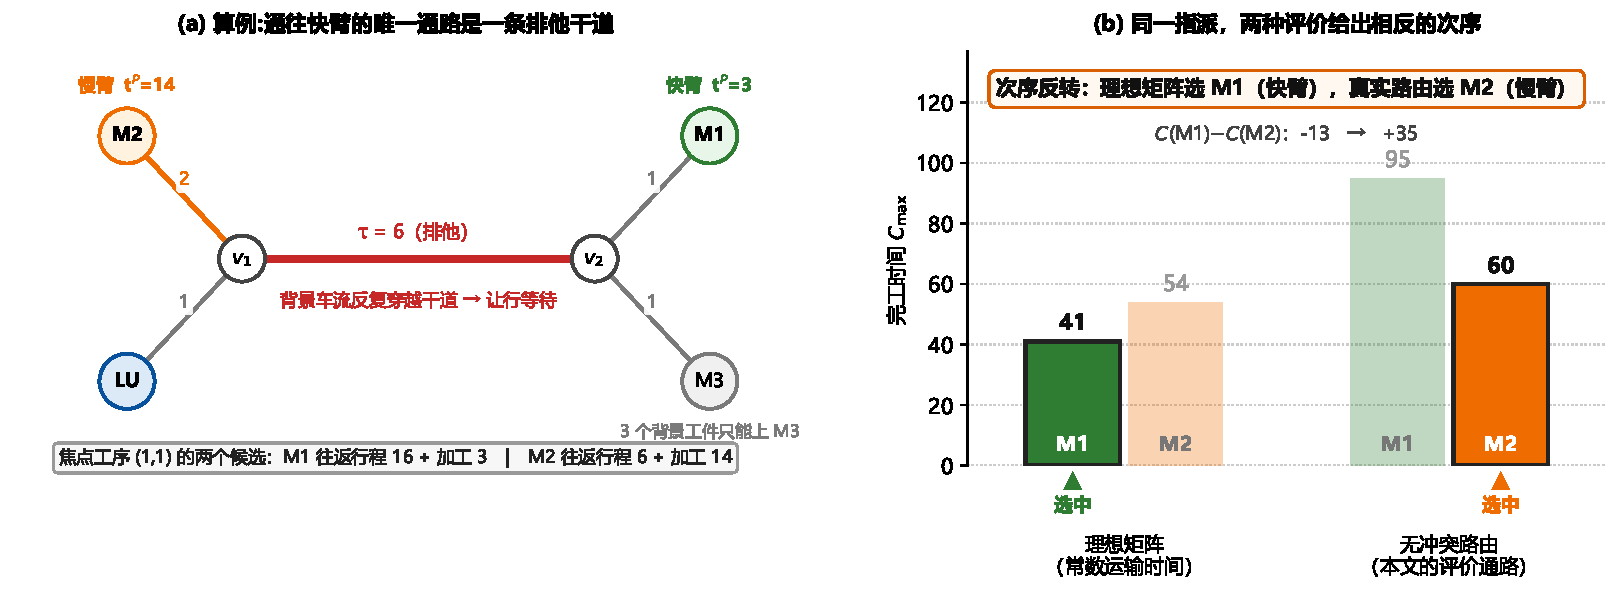
\includegraphics[width=\textwidth]{fig/fig_motivating.pdf}
\Description{Two panels. The left panel is a small shop network in which the only
route to a fast arm passes through an exclusive trunk corridor, while a slow arm
hangs on its own branch. The right panel shows makespan for the same two machine
assignments evaluated twice: under a constant travel-time matrix the fast arm
wins, under conflict-free routing the slow arm wins, so the ranking reverses.}
\caption{Motivating instance: the same assignment decision, ranked in opposite order by two evaluations.
(a)~The only path to the fast arm M1 is an exclusive trunk ($\tau=6$); the slow arm M2 sits on a short corridor that avoids the trunk; three further jobs that can only be processed on M3 must cross the trunk repeatedly.
(b)~The fast-arm and slow-arm assignments of the same operation, each evaluated by the constant matrix and by conflict-free routing.
The constant travel-time matrix contains no yielding wait, so it chooses the fast arm by ``shorter processing $+$ longer travel''; evaluating the same assignments by conflict-free routing makes the slow arm better.
The difference flips from $-13$ to $+35$.
This figure is an \emph{existence demonstration}, not a statistical conclusion---it shows that the reversal can occur, not that it must; of $1200$ parameter combinations around this instance, $205$ ($17\%$) reverse, so it is not an isolated point in the parameter space.}
\label{fig:motivating}
%% From fig/fig_motivating.py and clbs/output/motivating.json
%% (clbs/tools/motivating.py --sweep; same decoder as the paper).
%% Panel (b) numbers are not schematic: unimpeded matrix =
%% decode(conflict_free=False), conflict-free routing = decode(conflict_free=True).
%% Instance: 4 jobs / 3 arms / 6 nodes / 5 corridors / 2 AGVs, delta_return=1,
%% rule-based dispatching.  Do not reuse fig/fig_intro_problem_new.pdf
%% (previous paper, proximity-vs-availability, not corridor contention).
\end{figure*}

\subsection{Gap relative to prior work}

Existing work typically treats either the scheduling of a flexible job shop or the conflict-free travel of vehicles; when the two are combined, the assignment is usually fixed first and routing then absorbs the contention, so delay cannot go back and revise the schedule.
Writing flexible assignment and conflict-free routing into one problem, an existing exact method already solves small instances to proven optimality~\cite{vanos2026exact}; this paper adopts that existing problem setting, and the contribution is the solver, not the problem definition.
Once the instance size exceeds the range on which that exact decomposition can prove optimality, existing methods in the literature still split scheduling and conflict-free routing into two successive steps: the first stage fixes machine assignment and operation sequence, and the second stage then resolves vehicle conflicts for this already frozen schedule~\cite{sun2023integrated}.
The corridor contention seen by the second stage cannot go back and revise the machines and the sequence already chosen in the first stage.
Even when feedback is added, it only writes the transport durations of one execution back onto the time axis and acts on the current solution only; it neither revises the machine assignment nor repeats the step for every candidate in the search; the experimental benchmark is still one machine per operation, so reassignment does not exist~\cite{li2026framework}.
Thus the trade-off in which machine flexibility, heterogeneous processing efficiency, and corridor contention are present at once, and the schedule is optimized for the makespan after yielding wait is counted, has not been studied or stated in the existing literature.
The literature position is in Section~\ref{sec:Chapter_II}.

\subsection{Approach}

Against the gap that contention cannot go back and revise the schedule, and that the search does not count yielding wait, this paper connects scheduling and conflict-free routing by two paths and measures the contribution of each path to makespan separately.
The framework uses a bilevel structure---the upper level decides machine assignment and operation sequencing, the lower level generates conflict-free paths by time-window reservation---but connects the two levels along an evaluation path and a decision path, and reports the makespan change brought by each path separately.

The \emph{evaluation path} takes the fitness of each candidate as the makespan after the lower level has completed conflict-free routing, so yielding wait enters the objective that the search optimizes rather than a post-hoc feasibility check.
The computational cost of one conflict-free decode is about an order of magnitude higher than a decode on the unimpeded shortest-path matrix; under a fixed compute budget, a higher cost per evaluation reduces the number of evaluations that can be completed.
\cite{li2026framework} lists ``extending this mechanism into a fully iterative loop'' as future work, but does not report the computational cost of that practice or its effect on makespan.
This paper measures that trade-off under an equal wall-clock budget.

The \emph{decision path} uses \emph{reservation-table-aware vehicle dispatching}.
One transport consists of two legs, empty pickup and loaded delivery.
For each candidate vehicle, the lower-level router runs a trial query on the current reservation table for the earliest feasible times of the two legs in turn (the trial query does not write the final timetable), and chooses the vehicle with the earliest feasible delivery, rather than the vehicle whose arrival is earliest by the unimpeded-shortest-path estimate.
This rule replaces the idle-first dispatching used by~\cite{li2026framework}.
To keep each evaluation \emph{low-overhead} under an equal wall-clock budget, this paper gives two optimizations that do not change the output: admissible lower-bound pruning, and winner-path reuse.

Two further inter-layer interfaces are also implemented: first, an extra cost on occupied corridor--time slots, so that later paths avoid those slots; second, changing the processing machine or adjusting the operation sequence according to the corridor on which a yield occurred and the transport that occupied that corridor first.
Under an equal wall-clock budget, neither yields a stable makespan gain.
They are reported to show that thickening the inter-layer interface beyond the evaluation path and the decision path was not left untried, but did not convert into a makespan gain under the same budget;
the results are in Section~\ref{sec:Chapter_V}.

\subsection{Main results}

To measure the contribution of closed-loop evaluation and of reservation-table-aware dispatching separately, we construct a four-level baseline ladder, of which the first two levels reproduce the structure of two published works:
\textbf{B0} is open-loop planning plus actual execution, corresponding to~\cite{li2026framework};
\textbf{B0+} on a frozen schedule only replaces vehicle assignment with a conflict-aware one, corresponding to the two-stage structure of~\cite{sun2023integrated};
\textbf{B1} is closed-loop planning plus rule-based dispatching;
\textbf{B2} is the method of this paper.
The four levels are arranged along two factors: whether the search includes conflict-induced delay, and whether a vehicle is chosen by unimpeded time or by a trial query on the reservation table.
Therefore only a comparison that changes one factor at a time can attribute the gain to the corresponding mechanism.
The makespan that an open-loop plan reports of itself is often infeasible on the actual corridors.
Therefore every schedule is executed by the same conflict-free path planner, and what is compared is uniformly the realized makespan after execution.

The results show that the comparison on both factors yields a significant gain.
Moving congestion into the search objective (fixing the dispatching rule) reduces makespan by
\GainLoopRule{} ($p\PLoopRule$), which is the value of the closed loop itself;
within the closed loop, replacing rule-based dispatching with reservation-table-aware
dispatching (both are closed-loop, and only the vehicle-selection rule differs) reduces it by a further \GainProbeLoop{} ($p\PProbeLoop$),
which is the value of that specific mechanism;
end-to-end relative to the literature structure the reduction is \GainEndToEnd{}, \WinEndToEnd{} wins and
\LoseEndToEnd{} losses ($p\PEndToEnd$).
The two speed-ups bring the speedup of the dispatching mechanism to a factor of \SpeedupProbe{},
cut router calls by \RouteCallCut{}, and press the cost multiple per evaluation from \CostMultBefore{} to
\CostMultAfter{}, which is exactly why it can convert into a net gain under an equal wall-clock budget.

Both mechanisms are significant, but they are \emph{not substitutes for each other}.
Reservation-table-aware dispatching under the open loop is worth \GainProbeOpen{}
($p\PProbeOpen$), far smaller than the closed-loop \GainLoopRule{};
the end-to-end \GainEndToEnd{} is close to the \GainIndepProduct{} that the two would have if independent, is near-additive, and no positive interaction is detected.
The two factors are therefore reported separately, rather than as a single contrast from the open loop to the complete method---the latter would mix two gains of very different size into one (the few percentage points from dispatching would be covered by the closed loop), and only a separate report shows that the gain from dispatching is small but still significant.

Results reported separately by layout, vehicle-to-arm ratio, and flexibility are in Section~\ref{sec:whichcongestion}.
The two paths behave differently on the several instances.
When a significance test is run on each instance separately, a Holm correction is applied along the three axes above: without the correction, the probability of at least one ``significant'' finding among the \NCases{} instances would be far above the nominal level.
After correction, the closed-loop gain remains significant on \CellsSigLoopAdj{}/\NCases{} instances and rises roughly with contention intensity, so it can be read along the layout axis.
Reservation-table-aware dispatching is significant on none of the instances on its own (before correction, \CellsSigProbe{} instances);
on the four levels of the vehicle-to-arm ratio the gain is sometimes positive and sometimes negative, and none reaches significance.
Dispatching is significant only when the instances are pooled; with \NSeeds{} seeds per instance, the sample is not sufficient to identify on which class of instances the gain is stably positive.

The numbers above also depend on two comparison rules; the details are in Section~\ref{sec:protocol}.
First, the computational cost per evaluation of the methods can differ by about two orders of magnitude; comparing at the same search generation count is equivalent to giving the method whose evaluation is more expensive more compute.
This paper aligns on the same wall-clock interval.
Second, each contrast changes only one factor---whether the search includes delay, or how a vehicle is chosen; if a contrast changes both places at once, what is obtained is only a total, and it cannot be told whether the gain comes from the closed loop or from dispatching.

\subsection{Contributions}

\begin{enumerate}[leftmargin=*]

\item \textbf{At the problem layer: the reassignment trade-off when flexibility, heterogeneous efficiency, and corridor contention are present at once.}
When machine flexibility, heterogeneous processing efficiency, and corridor contention are present at once, and the schedule is optimized for the makespan after yielding wait is counted, if the corridor to a fast robotic arm is congested,
a slower arm with better connectivity may be the better assignment.
Models that schedule on a constant travel-time matrix cannot see this comparison---the matrix contains no yielding wait~\cite{sun2023integrated};
models that have conflict-free routing but a fixed machine per operation also lack this comparison, because reassignment does not exist~\cite{li2026framework}.
This paper adopts the existing setting of FJSP with conflict-free transportation constraints~\cite{vanos2026exact}; the contribution is the solver, not the problem definition;
and it supplements a controllable characterization of contention intensity, used to examine how high contention must be before counting yielding wait in the schedule yields a gain.

\item \textbf{At the framework layer: a closed-loop bilevel framework, and a measurement of the contribution of routing-in-the-loop evaluation to makespan.}
\emph{Routing-in-the-loop evaluation} takes the fitness of each candidate as the makespan after the lower level has completed conflict-free routing, so yielding wait enters the objective that the search optimizes.
The computational cost of one conflict-free decode is about an order of magnitude higher than a decode on the unimpeded shortest-path matrix; under a fixed compute budget, a higher cost per evaluation reduces the number of evaluations that can be completed.
\cite{li2026framework} lists ``extending this mechanism into a fully iterative loop'' as future work,
but does not report the computational cost of that practice or its effect on makespan.
This paper measures that trade-off under an equal wall-clock budget: relative to the open loop (the search ignores conflicts), the closed loop reduces makespan by \GainLoopRule{} ($p\PLoopRule$);
under reservation-table-aware dispatching, the closed loop relative to the open loop reduces it by \GainLoopProbe{} ($p\PLoopProbe$).

\item \textbf{At the mechanism layer: reservation-table-aware vehicle dispatching, and the two optimizations that keep it \emph{low-overhead}.}
Within the closed loop, replacing vehicle selection by unimpeded time with reservation-table-aware dispatching reduces makespan by a further \GainProbeLoop{} ($p\PProbeLoop$).
This rule replaces the idle-first dispatching used by~\cite{li2026framework}.
This paper gives two optimizations---admissible lower-bound pruning and winner-path reuse---and proves that they do not change the selected vehicle or the final timetable;
router calls fall by \RouteCallCut{}, the cost multiple per evaluation falls from \CostMultBefore{} to \CostMultAfter{}, and the speedup is \SpeedupProbe{}.
Vehicles have the same capability; they differ only in current position and corridor occupancy, so contention on the reservation table can decide which vehicle is chosen directly; reassigning a robotic arm also changes the processing time, and the processing-time gap is often larger than the corridor-wait gap.

\item \textbf{The closed loop and dispatching differ in the size of their contributions, and dispatching is not yet sufficient to identify on which class of instances the gain is stable.}
The closed loop remains significant after correction on \CellsSigLoopAdj{}/\NCases{} instances;
the gain of reservation-table-aware dispatching is much smaller, significant only when the instances are pooled, and the end-to-end value is close to the prediction when the two factors combine independently.
Changing only vehicle selection under the open loop is far from a substitute for counting yielding wait in the search.
After correction, dispatching is significant on none of the instances on its own (before correction, \CellsSigProbe{}/\NCases{} instances); on the four levels of the vehicle-to-arm ratio the gain is sometimes positive and sometimes negative.
Significance in the aggregate only shows that the direction of the mechanism is positive; with \NSeeds{} seeds per instance, the sample is not sufficient to identify on which class of instances the gain is stably realized.
The two paths are measured separately by the four-level baseline ladder.
Two inter-layer interfaces---an extra cost on occupied corridor--time slots, and reassignment or sequence adjustment from the yield record---are written into Section~\ref{sec:Chapter_V} as controls; under an equal wall-clock budget neither yields a stable gain.


\end{enumerate}

The notation of the paper is collected in Table~\ref{tab:notation}.



\section{Related work}
\label{sec:Chapter_II}

Related work falls into two strands.
One is flexible job shop scheduling with transportation times: it decides what is processed where and in what order; vehicles enter only as capacity resources, and travel times are taken from a constant matrix.
The other is conflict-free multi-robot routing: it resolves vehicle contention in space and time, but does not change the start, end, or release time of a task.
The two strands are reviewed in turn, then the work that puts both into one problem, and finally the gap that this paper fills.


\subsection{Flexible job shop scheduling with transportation}

The flexible job shop scheduling problem with processing machines and transport vehicles (FJSP\_PT) extends FJSP by bringing material movement into the schedule.
Xin et al.~\cite{xin2025review} systematically review progress in the field through 2023, organize its assumptions, constraints, objectives, and
benchmark instances, and divide solution methods into exact, heuristic, metaheuristic, and swarm-intelligence classes.
Modelling, constraints, and solution methods of the general flexible job shop are covered by a contemporaneous review~\cite{dauzereperes2024fjsp}.
The public benchmarks of this family are collected by Homayouni and Fontes~\cite{homayouni2021production}.
The dominant modelling convention among them
is a constant travel-time matrix indexed by location pairs: a vehicle needs a fixed $t(a,b)$ to move a job from $a$ to $b$,
which does not change with whether other vehicles occupy the same corridor.
Vehicles therefore enter the model only as capacity resources: a finite fleet competes for transport tasks, and occupancy of a corridor slot is not constrained.
% [ref_check: key=xin2025review; claim="review covers progress through 2023 and splits methods into exact/heuristic/metaheuristic/swarm-intelligence"; need=quote]
% [ref_check: key=xin2025review; claim="a constant travel-time matrix is the dominant modelling convention in FJSP_PT"; need=quote]

Under this modelling convention, solution methods have advanced quickly.
Meng et al.~\cite{meng2025cp} give a constraint-programming model of FJSP with multiple AGVs, close 29 previously open benchmark instances and improve 27 best-known solutions, and couple it with a dual-population genetic algorithm assisted by constraint programming.
Qin et al.~\cite{qin2026knowledge} combine a quality--diversity archive with Q-learning region
selection, and design a local search jointly guided by AGVs and the critical path---but that critical path is still computed on matrix travel times.
Fu et al.~\cite{fu2025integrated} use an improved genetic algorithm to decide production and
logistics jointly in a flexible assembly shop; the ``integration'' means that the two classes of decision are solved together, not that transport duration varies with the schedule.
In all of the work above, however, transport duration is read from the matrix, so one vehicle is never delayed by another through corridor contention.
% [ref_check: key=meng2025cp; claim="closes 29 previously open benchmarks and improves 27 best-known solutions"; need=quote]
% [ref_check: key=meng2025cp,qin2026knowledge,fu2025integrated; claim="all three take transport duration from a constant matrix; vehicles do not delay one another"; need=quote]

These assumptions, however, ``reduce the complexity of the problem and even change its nature''~\cite{xin2025review}; for example, when the number of transport vehicles is large enough, the time at which a job arrives at a machine is in practice affected by traffic congestion;
the dependence between the processing and transport stages must be handled first, or the plan that is produced cannot even be called feasible on the actual corridors.
% [ref_check: key=xin2025review; claim="the review lists the constant travel-time matrix as a limiting modelling choice, not a settled fact"; need=quote]
% [ref_check: key=xin2025review; claim="arrival times at machines are affected by congestion; the processing-transport dependence must be handled first"; need=quote]

This strand of the literature has machine flexibility, but it schedules on a constant travel-time matrix, and can therefore push machine assignment and operation sequencing very far.
The matrix contains no yielding wait:
two transports do not postpone each other through contention, and the ranking of an assignment does not change with corridor occupancy.
This paper keeps its flexible modelling and its metaheuristic solution framework, and only replaces the constant transport duration in the matrix with the traversal time after conflict-free routing---which may contain yielding wait caused by other vehicles.

\subsection{Conflict-free routing with exogenous tasks and congestion-aware dispatching}

The other strand takes corridor contention itself as the object.
Multi-agent path finding (MAPF) requires several agents to walk from start to goal without collision on a shared graph; optimal solution is NP-hard~\cite{gao2023mapf};
for a single vehicle finding a path on an already occupied graph, recent work attaches Safe Interval Path Planning to two-dimensional road networks and continuous time~\cite{kasaura2022sipp}.
Especially in settings with continuously arriving tasks, congestion already reduces the number of tasks completed per unit time when the network is far from saturation.
Zhang et al.~\cite{zhang2024guidance} optimize a road network with edge weights, use the weights to steer agents away from bottlenecks and reduce head-on meetings, and thereby let several solvers of continuously arriving tasks complete more tasks.
In a manufacturing setting, Kim and Kim~\cite{kim2026congestion} give a congestion function, a congestion penalty, and congestion-aware dispatching rules for a large AGV fleet, and evaluate them in discrete-event simulation.
A survey of multi-AGV management lists dispatching as a layer independent of path planning, and idle-first and nearest-vehicle as common single-attribute rules among them~\cite{lu2022agv};
a survey of planning and control of autonomous mobile robots lists task allocation and path planning as adjacent layers on the same control stack~\cite{fragapane2021planning}.
% [ref_check: key=zhang2024guidance; claim="in lifelong MAPF, congestion already hurts throughput far below capacity"; need=quote]
% [ref_check: key=zhang2024guidance; claim="the guidance graph suppresses head-on motion and raises throughput of several lifelong solvers"; need=quote]

Two points of this strand are directly relevant to this paper.
First, the release time, start, and end of a task are inputs to the router; the router cannot change the machine assignment that produced those tasks.
Second, congestion is usually quantified not by the yielding wait that actually occurred on a transport, but by an indirect measure: \cite{kim2026congestion} looks at local vehicle density, and \cite{zhang2024guidance} uses offline-learned edge weights of the road network (the larger the weight, the less a vehicle is encouraged to take that edge).
Density or an edge weight can only show that a corridor has relatively many vehicles; a yield can name which corridor, which interval, and which transport occupied it first.
% [ref_check: key=zhang2024guidance,kim2026congestion; claim="release times and endpoints are exogenous; the router does not generate tasks"; need=quote]
% [ref_check: key=kim2026congestion; claim="their congestion measure is local vehicle density"; need=quote]
% [ref_check: key=zhang2024guidance; claim="guidance-graph edge weights are learned offline, not updated online"; need=quote]

This strand has genuine conflict-free routing, but has no flexibility: tasks arrive from elsewhere, and assignment is outside its decision scope.
This paper keeps its conflict-free path generation, and lets the upper-level schedule change the assignment and the operation sequence from the yields that occur in the routing.

\subsection{Integrating scheduling and conflict-free routing: feedback depth and our position}

Work that writes flexible assignment and conflict-free routing into one problem is scarce.
van Os and Basten~\cite{vanos2026exact} formalize FJSP with conflict-free transportation constraints: an operation has optional machines and a processing time that varies with location, and vehicles must travel conflict-free.
The solver uses logic-based Benders decomposition---a constraint-programming master gives machine assignment and operation sequence, and an integer-programming subproblem plans conflict-free paths for that schedule;
if a path is infeasible, the subproblem writes the conflict as a new constraint and sends it back to the master, forbidding a schedule of the same kind.
Most benchmark instances are solved to proven optimality, and about half of them improve makespan by at least $10\%$ relative to prior heuristics.
The method is limited by the instance size on which the exact decomposition can prove optimality.
The authors note that making fuller use of the information ``which conflicts caused the infeasibility'' is a natural follow-up.
This paper adopts that existing problem setting; the contribution is the solver: on sizes that the exact decomposition cannot reach, a heuristic sends the delay in the routing back into the scheduling decision.
% [ref_check: key=vanos2026exact; claim="most benchmarks solved to proven optimality; about half improve makespan by at least 10% over prior heuristics"; need=quote]
% [ref_check: key=vanos2026exact; claim="applicable size is limited by what the exact decomposition can reach"; need=quote]

Once the instance size exceeds that exact decomposition, existing heuristics still split scheduling and conflict-free routing into two successive steps.
Sun et al.~\cite{sun2023integrated} first fix machine assignment and operation sequence by a hybrid genetic algorithm, then resolve conflicts by a genetic algorithm with an AGV encoding and time-window Dijkstra;
the contention seen by the second stage cannot go back and change the machines and the sequence already chosen in the first stage.
Li et al.~\cite{li2026framework} add one feedback: the path layer writes the realized transport durations back onto the time axis, only shifts start times, does not change the machine assignment, and acts on the current solution only;
the benchmark is still one machine per operation, so reassignment does not exist.
% [ref_check: key=sun2023integrated; claim="second-stage conflict resolution does not revise first-stage schedule or assignment"; need=quote]
% [ref_check: key=li2026framework; claim="feedback is time only; the experimental benchmark has one optional machine per operation"; need=quote]

The gap left by existing work is not whether vehicle conflicts are handled, but how the routing result enters the schedule.
Sun~\cite{sun2023integrated} and Li~\cite{li2026framework} have both brought conflict-free travel into the pipeline; the difference is the number and the content of the feedback---whether every candidate is evaluated by actual routing, or only the current solution is done once;
whether only transport durations are written back, or the schedule can change the machine assignment from them.

Critical-chain reasoning is a mature device in job-shop local search~\cite{otala2021graph,tamssaouet2023neighborhood}, and recent FJSP work with transportation times uses it as well~\cite{qin2026knowledge}.
But if the critical chain is computed on a constant travel-time matrix, a start delay can be traced only to a slow predecessor or a busy machine, not to a corridor---the matrix contains no corridor occupancy.
After this paper switches to conflict-free routing by time-window reservation, the same delay can fall on a concrete segment, a concrete interval, and the transport that occupied that segment first.
% [ref_check: key=qin2026knowledge; claim="critical-chain reasoning is a mature device in job-shop local search"; need=quote]

On instance design, \cite{xin2025review} notes that instances in the field ``differ mainly in size and lack a dedicated design for the values of key problem
parameters'', and in particular lists the ratio of mean transport time to mean processing time $\bar{T}_t/\bar{T}_p$ as a quantity that is highly likely to affect algorithm performance, and calls for an expanded test set.
On top of this, this paper supplements a parameter that is visible only after routing is modelled explicitly: how much of an instance's congestion is assignment-related.
Congestion concentrated at the load/unload exit is crossed by every job under every assignment, and therefore rewards no decision; congestion on a corridor that serves only some machines can be bypassed.
Two instances with identical $\bar{T}_t/\bar{T}_p$ may leave the scheduling mechanism completely different room to act.
This paper therefore generates instances whose contention intensity is controllable (Section~\ref{sec:Chapter_V}).
% [ref_check: key=xin2025review; claim="the review lists mean transport over mean processing time as likely to affect performance and calls for a larger test set"; need=quote]

Table~\ref{tab:related} summarizes the comparison above.
The problem setting adopts the FJSP with conflict-free transportation constraints already formalized by~\cite{vanos2026exact}; the contribution is not the problem definition.
What is open is the size that the exact decomposition cannot reach: here the connection between scheduling and routing is still either missing, or only schedule-then-resolve, or only one feedback on the current solution.
This paper gives a bilevel framework at that size: every candidate is evaluated by the makespan after conflict-free routing, and reservation-table-aware dispatching chooses a vehicle by a trial query; the two optimizations press down the cost per evaluation and do not change the selected vehicle or the timetable.
Closed-loop evaluation is the larger effect, dispatching is a smaller but still significant effect, and the two are measured separately.

\begin{table}[t]
  \caption{Comparison of related work with this paper.
``Machine heterogeneity'' means that an operation has several optional machines and the processing time varies with the machine;
``coupling frequency'' means the number and direction of times the routing result enters the schedule;
the last column is the content fed back to the schedule.
This paper evaluates every candidate by the makespan after conflict-free routing, and chooses a vehicle by reservation-table-aware dispatching.
This paper implements three interfaces---realized time, the yield record, and a surcharge on corridor--time slots---and reports each by its cost and its gain.}
\label{tab:related}
%% Hand-maintained table: no generator.  Any row change must match Section 2.3.
\footnotesize
\begin{tabular}{@{}lclll l@{}}
\toprule
Work class & Ref. & Machine het. & Vehicle contention & Coupling freq. & Feedback content \\
\midrule
FJSP\_PT metaheuristics & \cite{meng2025cp,qin2026knowledge,fu2025integrated}
  & yes & constant matrix & --- & --- \\
Lifelong MAPF & \cite{gao2023mapf,zhang2024guidance}
  & --- & conflict-free & tasks exogenous & edge weights \\
Congestion-aware dispatching & \cite{kim2026congestion}
  & no & density proxy & one-way & congestion penalty \\
Two-stage FJSP + routing & \cite{sun2023integrated}
  & yes & conflict-free & one-way & none \\
RL scheduling + PBS & \cite{li2026framework}
  & no & conflict-free & one-shot correction & arrival times \\
Exact LBBD & \cite{vanos2026exact}
  & yes & conflict-free & master--subproblem & conflict-driven cuts \\
\textbf{This paper} &
  & yes & conflict-free & every candidate & realized time + trial query \\
\bottomrule
\end{tabular}
\end{table}


\section{Problem statement and model}
\label{sec:Chapter_III}
\subsection{Problem statement}

An instance consists of $n$ jobs, $N_M$ robotic arms, and $N_A$ automated guided vehicles, operating on a shop-floor road network represented as a graph.
Job $j$ has a fixed chain of $n_j$ operations $O_{j1}\to\cdots\to O_{jn_j}$; operation $O_{ji}$ may be processed on any robotic arm in its option set $\Omega_{ji}\subseteq M$, taking time $t^P_{jim}$ on arm $m$, a value that depends on the chosen arm.
Robotic arms occupy fixed nodes of the graph; jobs are moved between these nodes by the fleet.
Solving an instance means determining four groups of decisions at once:

\begin{enumerate}[label=(\roman*),leftmargin=*,topsep=2pt,itemsep=1pt]
\item assign each operation $O_{ji}$ to some robotic arm $m\in\Omega_{ji}$;
\item sequence the operations assigned to each robotic arm;
\item assign the induced transport tasks to vehicles and sequence the tasks of each vehicle;
\item plan a path on the graph for every vehicle move, requiring temporal and spatial conflict-freedom and allowing waits.
\end{enumerate}

The objective is to minimize the makespan $C_{\max}$.

\begin{table}[t]
\caption{Notation.}
\label{tab:notation}
\small
\begin{tabular}{@{}ll@{}}
\toprule
Symbol & Meaning \\
\midrule
$J=\{1,\dots,n\}$, $O_{ji}$ & set of jobs; the $i$-th operation of job $j$, $i\le n_j$ \\
$M=\{1,\dots,N_M\}$, $\Omega_{ji}\subseteq M$ & set of robotic arms; option set of $O_{ji}$ \\
$t^P_{jim}$ & processing time of $O_{ji}$ on arm $m\in\Omega_{ji}$ \\
$K=\{1,\dots,N_A\}$ & homogeneous unit-load vehicles \\
$G=(V,E)$, $\tau_e$ & shop-floor graph; traversal time of corridor $e\in E$ \\
$v_0$, $\mathrm{loc}(m)$ & load/unload station; node occupied by arm $m$ \\
$t^{*}(a,b)$ & shortest-path time from $a$ to $b$ in $G$, ignoring contention \\
$\delta_{\mathrm{ret}}\in\{0,1\}$ & whether a finished job returns to $v_0$ (baseline value $1$) \\
$S_{ji}$, $C_{ji}$, $A_{ji}$ & start, completion, and material-arrival times of $O_{ji}$ \\
$C_{\max}$ & makespan \\
\bottomrule
\end{tabular}
\end{table}

\subsection{Modelling assumptions}
\label{sec:assumptions}

\begin{enumerate}[label=\textbf{A\arabic*.},leftmargin=*,topsep=2pt,itemsep=2pt]
\item \textbf{Static instance and complete information.} All $n$ jobs are already at $v_0$ at time $t=0$; there are no release dates or due dates. Processing data, the layout $G$, and the vehicle states are known at planning time.

\item \textbf{Jobs.} Each job has a fixed precedence chain. Processing and transport are non-preemptive; jobs cannot be split; there are no exogenous precedence constraints among different jobs.

\item \textbf{Robotic arms: partial flexibility and heterogeneous processing times.} Each operation $O_{ji}$ may be processed on any $m\in\Omega_{ji}$; most operations satisfy $|\Omega_{ji}|\ge 2$, and full flexibility $\Omega_{ji}=M$ is a special case. Processing times depend on the chosen arm, and the arms need not share a uniform ranking by speed: when $m\neq m'$, $t^P_{jim}$ and $t^P_{jim'}$ need not be proportional. An arm processes only one operation at a time, does not fail during the planning horizon, and sequence-dependent setup is folded into $t^P_{jim}$.

\item \textbf{Buffers and loading.} The input and output buffers of each arm, and the storage at $v_0$, have ample capacity, so blocking does not occur. Loading and unloading times are negligible and do not occupy the arm.

\item \textbf{Vehicles.} The $N_A$ vehicles are homogeneous and unit-load; they travel at constant speed whether empty or loaded; acceleration, deceleration, and battery charge are not modelled. All vehicles stand empty at $v_0$ at $t=0$ and are immediately available. A transport task is a one-way move---from $v_0$ to the first arm, between two successive distinct arms, or, when $\delta_{\mathrm{ret}}=1$, from the last arm back to $v_0$; any vehicle may execute any task, so successive moves of the same job may be relayed across different vehicles. After unloading, a vehicle is not forced back to $v_0$; it repositions according to its own task chain, and its departure time may be postponed by the routing layer.

\item \textbf{Road network and conflict-freedom.} $G$ is strongly connected; the traversal time $\tau_e$ of each corridor is a known constant. Corridors are \emph{exclusive} resources: the two directions of $e$ share a single reservation, so at most one vehicle occupies $e$ at any time, which rules out both head-on conflicts and same-direction overtaking. Occupancy intervals are half-open, $[t,\,t+\tau_e)$, so a second vehicle may enter exactly at $t+\tau_e$. Nodes have ample berths, independent of the traversal resource; waits therefore occur at berths and are always permitted.

\item \textbf{Out of scope.} Machine and vehicle failures, finite buffers and blocking, battery charging, and dynamic job arrivals~\cite{gui2023dynamic,xiong2024dynamic} are left to future work (item~(5) of Section~\ref{sec:future_work}).
\end{enumerate}

Of these, A1, A2, A4, and A5 are standard assumptions in the FJSP\_PT literature~\cite{xin2025review}.
What actually shapes this paper is A3 (machine-dependent processing times on partially flexible robotic arms) and A6 (contention stated as an explicit exclusive-resource constraint, not as a constant travel-time matrix), together with the fact that follows: transport duration is an output of the routing decision, not a fixed input parameter.
Deadlock-freedom is not listed as an assumption.
A4 and A6, together with Proposition~\ref{prop:decodable} in Section~\ref{sec:router}, show that any assignment and operation sequence can be decoded into a conflict-free, deadlock-free timetable, so the search need not repair infeasible solutions.

\subsection{Decision variables and induced transport tasks}

Let $x_{jim}\in\{0,1\}$ indicate that $O_{ji}$ is assigned to robotic arm $m$; write $\mathrm{m}(j,i)$ for the chosen arm and $d_{ji}=\mathrm{loc}(\mathrm{m}(j,i))$ for the node of that arm.
When $\delta_{\mathrm{ret}}=1$, a zero-duration \emph{dummy operation} $O_{j,n_j+1}$ at $v_0$ is appended to each job, representing the return to the load/unload station after completion;
in this way return moves and intermediate moves share the same task notation, and the makespan is always the completion time of each job's last operation.

Unlike a vehicle routing problem, transport tasks are not part of the input; they are \emph{induced} by the assignment:
\begin{equation}
\label{eq:tasks}
\mathcal{T}(x)=\Bigl\{\,(j,i)\ :\ d_{j,i-1}\neq d_{ji}\,\Bigr\},
\qquad d_{j0}\equiv v_0 ,
\end{equation}
where task $(j,i)$ moves job $j$ from $d_{j,i-1}$ to $d_{ji}$ and becomes ready at time $r_{ji}=C_{j,i-1}$ (with the convention $C_{j0}=0$).
If two successive operations are placed on the same arm, no transport task is created.
Thus both the \emph{number} and the \emph{endpoints} of transport tasks are consequences of decision group~(i): an assignment that keeps a job on the same arm throughout needs only two moves, whereas an assignment that changes arm at every operation needs $n_j+1$ moves.
Assignment of tasks to vehicles is indicated by $y_{tk}\in\{0,1\}$, with $\sum_{k\in K}y_{tk}=1$ for each $t\in\mathcal{T}(x)$; tasks given to the same vehicle are ordered into a sequence.

In a constant travel-time matrix model, the assignment likewise determines how many moves occur and from where to where, but the duration of each move is a constant in the matrix, and corridor occupancy does not enter the model.
In this paper, the same assignment also determines on which corridors those moves contend with one another.

\subsection{Timing relations and feasibility}

Write $p_{ji}=\sum_{m\in\Omega_{ji}}x_{jim}t^P_{jim}$ for the processing time on the chosen arm. Assignment, precedence, and the unit-capacity of each arm give
\begin{align}
\sum_{m\in\Omega_{ji}} x_{jim} &= 1, & \forall j,i,
\label{eq:assign}\\
C_{ji} &= S_{ji}+p_{ji}, & \forall j,i,
\label{eq:dur}\\
S_{ji} &\ \ge\ A_{ji}, & \forall j,i,
\label{eq:material}\\
S_{j'i'}\ \ge\ C_{ji}\ \ \vee\ \ S_{ji} &\ \ge\ C_{j'i'}
& \forall (j,i)\neq(j',i')\ \text{on the same arm},
\label{eq:disj}
\end{align}
where $A_{ji}$ is the time at which the job actually appears at $d_{ji}$.
If $(j,i)\notin\mathcal{T}(x)$, the job is already there and $A_{ji}=C_{j,i-1}$.
Otherwise $A_{ji}$ is produced by the vehicle that carries task $(j,i)$: write $a^{\mathrm{E}}_{ji}$ for the time at which that vehicle reaches the pickup node after its empty leg, and set
\begin{equation}
\label{eq:load}
\ell_{ji}=\max\bigl(a^{\mathrm{E}}_{ji},\ r_{ji}\bigr),
\qquad
A_{ji}=\text{arrival time of the loaded leg departing at }\ell_{ji},
\end{equation}
i.e.\ the vehicle may wait for the job, and the job may wait for the vehicle.
Whether empty or loaded, each leg is a walk $(e_1,\dots,e_q)$ in $G$ whose corridor entry times $\eta_1,\dots,\eta_q$ satisfy
\begin{equation}
\label{eq:walk}
\eta_1 \ \ge\ \sigma, \qquad
\eta_{l+1}\ \ge\ \eta_l+\tau_{e_l}, \quad l=1,\dots,q-1,
\end{equation}
where $\sigma$ is the time at which the leg may start;
if the entry time of the next corridor equals the time at which the current corridor is finished, there is no intermediate stop; if it is later, the difference is a wait at a berth.
The leg ends at $\eta_q+\tau_{e_q}$.
Finally, the corridor-contention constraint is
\begin{equation}
\label{eq:excl}
\bigl[\eta,\ \eta+\tau_e\bigr)\ \cap\
\bigl[\eta',\ \eta'+\tau_e\bigr)\ =\ \emptyset
\end{equation}
This equation holds for any two distinct occupancies of the same corridor $e$, independently of direction and of which vehicles are involved.
The objective is
\begin{equation}
\label{eq:obj}
\min\ C_{\max},\qquad
C_{\max}=\max_{j\in J}\ C_{j,\,n_j+\delta_{\mathrm{ret}}} .
\end{equation}

Two corollaries are worth recording, because the algorithms of Section~\ref{sec:Chapter_IV} rest on them.
First, in any semi-active schedule, \eqref{eq:material} and \eqref{eq:disj} tighten to
\begin{equation}
\label{eq:bind}
S_{ji}=\max\bigl(A_{ji},\ F_{\mathrm{m}(j,i)}\bigr),
\end{equation}
where $F_m$ is the completion time of the operation sequenced immediately before $O_{ji}$ on arm $m$.
Thus the start time equals the later of the job's arrival time and the completion time of the preceding operation on that arm; which of the two is later is settled by a comparison.
Later sections use this to attribute a postponed start to waiting for material or waiting for the arm.
Second, \eqref{eq:excl} is the only constraint in the model that couples different jobs through \emph{space} rather than through a shared machine.

\subsection{Relation to FJSP\_PT}
\label{sec:fjsppt}

After \eqref{eq:excl} is removed, legs no longer occupy corridors against one another, so each leg may take a shortest path and need not wait in between.
Transport durations collapse to the constant matrix $t^{*}(a,b)$, and the model becomes flexible job shop scheduling with transportation (FJSP\_PT).
The two problems therefore differ only in this set of corridor-exclusivity constraints: with them, the duration of a move is jointly determined by the vehicles' paths; without them, the duration is an input parameter.
The resulting $t^{*}$ is used later as a lower bound, and in the open-loop baseline to estimate arrival times by unimpeded travel time.
This paper adds these constraints to FJSP\_PT and adopts that problem setting.

Relative to work that likewise supplies an explicit road network, the difference lies in what is reserved.
van Os and Basten~\cite{vanos2026exact} reserve \emph{nodes}: two vehicles may not occupy the same node at the same time, nor swap nodes.
This paper reserves \emph{edges}: corridors are exclusive in both directions, and at most one vehicle occupies a corridor at any time.
Lyu et al.~\cite{lyu2019approach} likewise use a bidirectional network with edge exclusivity, but additionally require that a node hold at most one vehicle at a time; this paper does not impose that node-capacity constraint, and waits occur at ample berths.
Why the instances cannot be compared directly is explained under limitation~(1) of Section~\ref{sec:limitations}.

\subsection{Computational complexity}

\begin{prop}
\label{prop:np_hard}
The problem defined by \eqref{eq:assign}--\eqref{eq:obj} is strongly NP-hard; it remains so when every operation satisfies
$\Omega_{ji}=M$.
\end{prop}

\begin{proof}
Restrict to instances in which $\tau_e=0$ for every $e\in E$, each robotic arm is connected to $v_0$ by a dedicated corridor,
and $N_A=n$.
Every leg then has duration zero and occupies the empty half-open interval $[t,t)=\emptyset$, so \eqref{eq:excl}
holds identically and no vehicle can delay another; moreover, because each job has a dedicated vehicle, \eqref{eq:load} never binds,
and $A_{ji}=C_{j,i-1}$.
What remains is exactly \eqref{eq:assign}--\eqref{eq:disj} with $A_{ji}=C_{j,i-1}$, i.e.\ the flexible job shop scheduling problem with unrelated machines.
Two special cases of that problem are already strongly NP-hard: taking $|\Omega_{ji}|=1$ everywhere reduces it to the classical job shop, which is strongly NP-hard already with three machines; taking $\Omega_{ji}=M$ and $n_j=1$ reduces it to minimizing makespan on unrelated parallel machines, which contains identical-parallel-machine scheduling and is strongly NP-hard when the number of machines is part of the input.
Flexible job shop scheduling in general is itself strongly NP-hard~\cite{dauzereperes2024fjsp}.
Each of the restrictions above is a polynomial reduction, so the general problem is strongly NP-hard; the second special case also shows that full flexibility does not make the problem easy.
\end{proof}

The reduction of Proposition~\ref{prop:np_hard} sets corridor traversal times to zero and thereby excludes vehicle contention.
This shows that the problem is already strongly NP-hard even without corridor contention.
After decisions~(i)--(iii) are further fixed, the remaining path planning is still a conflict-free multi-agent routing problem~\cite{gao2023mapf}, and the release times and endpoints of the tasks are determined by the operation chains and the assignment, so they constrain one another.
Conflict-free routing therefore adds constraints on top of the scheduling hardness; it does not replace it.
Exact methods already exist at small scale: van Os and Basten~\cite{vanos2026exact} use logic-based Benders decomposition and solve most benchmarks under the same problem setting to proven optimality.
This paper addresses a scale beyond the reach of that exact decomposition.

\subsection{Instance features}
\label{sec:features}

This paper holds instance size fixed and varies only structure; the effect of size itself is discussed under limitation~(1) of Section~\ref{sec:limitations}.
Each instance records the following features.
The first four are quantities common in the scheduling literature; Xin et al.~\cite{xin2025review} note that $\bar{T}_t/\bar{T}_p$ in particular is likely to affect algorithm performance.


\begin{itemize}[leftmargin=*,topsep=2pt,itemsep=1pt]
  \item $\bar{T}_t/\bar{T}_p$: the mean shortest-path travel time among arm nodes divided by the mean processing time, i.e.\ the ratio of transport time to processing time.
  \item Heterogeneity $H$: the coefficient of variation of each operation's processing times over its optional arms, then averaged over all operations (operations with $|\Omega_{ji}|=1$ contribute $0$).
  $H=0$ means that optional arms have identical processing times, so reassignment no longer has a processing-time gain or loss, but an arm may still be changed to avoid congestion, and that change then costs no extra processing time.
  The measurements grouped by $H$ in Section~\ref{sec:whichcongestion} agree with this, so a larger $H$ is not expected to yield a larger gain.
  \item Flexibility $F=\operatorname{mean}_{ji}|\Omega_{ji}|/N_M$: the mean number of optional arms per operation as a fraction of all arms, i.e.\ the scope of reassignment.
  \item $N_A/N_M$: the vehicle-to-arm ratio. A smaller ratio makes the bottleneck more likely to lie in transport; a larger ratio, in processing.
\end{itemize}

In addition to the four items above, we record two quantities that are meaningful only on an explicit road network.
What matters is not how severe the congestion is, but how much of it can be avoided by reassignment.
Let $\mathrm{cut}(v_0)$ be a smallest set of corridors whose deletion disconnects the load/unload station $v_0$ from every robotic arm.

\begin{itemize}[leftmargin=*,topsep=2pt,itemsep=1pt]
  \item Contention intensity: on the initial random population, the share of total travel time that is yielding wait. It is read off from the instance structure, not supplied as an input; this paper uses it to order instances, and the per-instance values are in Table~\ref{tab:instances}.
  \item $|\mathrm{cut}(v_0)|$ (funnel width): an upper bound on the number of vehicles that can leave the load/unload station at the same time. The value $1$ means that every vehicle must pass through the same corridor to leave. The layout factor varies contention precisely by adding or removing such parallel exits; relative to \texttt{high}, \texttt{funnel} halves this value.
\end{itemize}

We also record a quantity that was tried and not adopted.
The \emph{funnel share} $\varphi\in[0,1]$ is, on a typical $v_0\to$arm trip, the fraction of time spent on corridors that are shared by \emph{every} shortest $v_0\to$arm path.
Such corridors are traversed by every job under any assignment, and the delay on them does not change with decisions~(i)--(iii); the larger $\varphi$, the harder it is for reassignment to avoid congestion.
It was intended to separate avoidable from unavoidable congestion, which contention intensity cannot do.
On the instances of this paper, however, two layouts that should differ by construction give almost the same $\varphi$, so it does not enter the later analysis and is recorded here only as a definition.
Designing a measure that distinguishes these two classes of layout is listed as future work (item~(1) of Section~\ref{sec:future_work}).
A far-group cut---the fewest corridors whose deletion isolates those arms whose distance to $v_0$ exceeds the median---was also tried, to describe bottleneck capacity away from the load/unload station;
under the single layout template of this paper it is almost identical to $|\mathrm{cut}(v_0)|$ and likewise does not enter the analysis.

Each instance carries a composite lower bound
$\mathrm{LB}=\max(\mathrm{LB}_{\text{chain}},\mathrm{LB}_{\text{load}},
\mathrm{LB}_{\text{cut}})$, computed directly from the instance data.
The three components each relax a different part of the model; none is always the largest on every instance.
$\mathrm{LB}_{\text{chain}}$ takes, for each job, ``the shortest inbound trip $+$
$\sum_i \min_{m\in\Omega_{ji}}t^P_{jim}$ $+$ the shortest return trip'', i.e.\ it ignores inter-arm moves and all queues.
$\mathrm{LB}_{\text{load}}$ takes $\sum_{j,i}\min_m t^P_{jim}/N_M$, i.e.\ it ignores operation precedence and transport.
$\mathrm{LB}_{\text{cut}}$ uses the funnel: when $\delta_{\mathrm{ret}}=1$ each job crosses
$\mathrm{cut}(v_0)$ twice; spreading $X=2n$ crossings over the corridors of that cut so as to minimize the load on the busiest one yields
\begin{equation}
\label{eq:lbcut}
C_{\max}\ \ge\ X\Bigl/\sum_{e\in \mathrm{cut}(v_0)}\tau_e^{-1}.
\end{equation}
On the instances of this paper, the largest of the three is $\mathrm{LB}_{\text{cut}}$ (eight of ten instances) or
$\mathrm{LB}_{\text{chain}}$ (the other two); $\mathrm{LB}_{\text{load}}$ is never the largest---which agrees with an instance design that concentrates contention at the load/unload exit.
The bound is loose: the gap to the best known solution is roughly between \LBGapLo{} and \LBGapHi{}, so it is used only to check the order of magnitude, not to prove that a solution is near-optimal.

\section{Closed-loop bilevel framework}
\label{sec:Chapter_IV}
\subsection{Overview: routing-in-the-loop evaluation and the decision path}
\label{sec:overview}

The framework assigns the four groups of decisions of Section~\ref{sec:Chapter_III} to two levels.
The input is an instance: the operation chains of the jobs, the option sets and processing times of the arms, the fleet size, and the corridor network.
The upper level searches over assignment and sequencing with a memetic algorithm~\cite{zhang2024memetic}; an event-driven decoder in the middle translates an upper-level candidate into a sequence of precedence-constrained transport tasks; the lower level turns that sequence into conflict-free paths by time-window reservation.
The output is an executable conflict-free timetable and its makespan.
Relative to two-stage schemes or schemes that correct only once, the difference is not that there are two levels, but how the routing result enters the schedule: what is fed back, along which path, and whether every candidate is fed back once.


\begin{description}[leftmargin=0pt,topsep=3pt,itemsep=3pt]
  \item[The evaluation path, i.e.\ \emph{routing-in-the-loop evaluation}.]
  In every generation, the fitness of every candidate is the makespan after the lower level has completed conflict-free routing of all transport tasks, yielding wait included.
  That is the number the upper level optimizes, not the makespan computed from unimpeded shortest paths.
  \item[The decision path.]
  Vehicle selection may read the current reservation table, rather than waiting until paths have been generated and then inspecting the result.
  The mechanism is \emph{reservation-table-aware vehicle dispatching}: for each candidate vehicle, a two-leg trial query is run on the reservation table to obtain the earliest feasible times of the empty and loaded legs (the trial query does not write the final timetable), and the vehicle with the earliest feasible delivery is chosen, rather than the vehicle whose arrival is earliest by the unimpeded-shortest-path estimate.
\end{description}

The evaluation path lets the search optimize the makespan after yielding wait is included; the decision path lets vehicle selection rest on a trial query on the reservation table, not on an unimpeded-time estimate.
The contribution of the two paths to makespan is measured separately in Section~\ref{sec:Chapter_V}: closed-loop evaluation is the larger effect, reservation-table-aware dispatching is a smaller but still significant effect, and the end-to-end gain is close to the value predicted when the two factors combine independently.
Changing only vehicle selection under the open loop is far from a substitute for bringing yielding wait into the search.

Two further inter-layer interfaces were also implemented: first, an extra cost on occupied corridor--time slots (hereafter, a surcharge), so that later paths avoid those slots; second, reassignment or reordering from the yield record.
Under an equal wall-clock budget, neither yields a stable makespan gain.
The constructions are in Sections~\ref{sec:interface} and~\ref{sec:ls}; the results appear as controls in Section~\ref{sec:Chapter_V}.

The structure of the framework is shown in Figure~\ref{fig:framework}.
The two paths enter the upper level at different places, and the computational cost of a single evaluation therefore differs as well.

%% From fig/fig_framework.py; a schematic, no data.
%% Do not reuse fig/fig_hdp_architecture*.pdf (HDP framework of a previous paper).
\begin{figure*}[t]
\centering
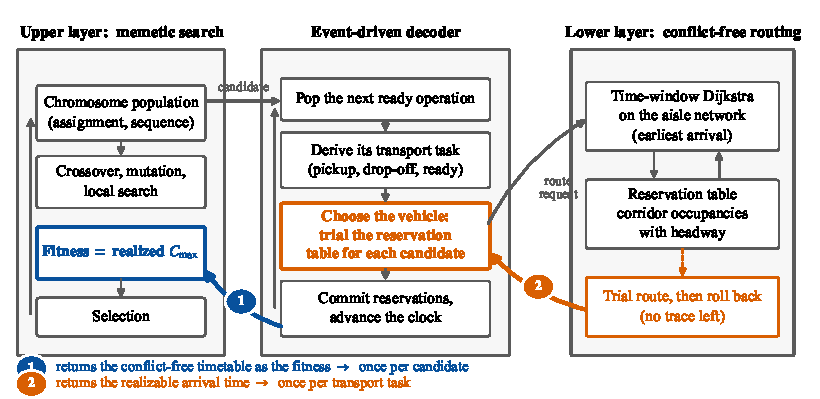
\includegraphics[width=\textwidth]{fig/fig_framework.pdf}
\caption{The closed-loop bilevel framework.
The upper level searches over assignment and sequencing with a memetic algorithm; the lower level performs conflict-free routing by time-window reservation; an event-driven decoder in the middle translates an upper-level candidate into a sequence of transport tasks.
The two feedback paths are distinguished by colour and enter the upper level at different places:
path~1 (blue, marked 1) returns the completed conflict-free timetable as fitness, once per candidate;
path~2 (orange, marked 2) runs a two-leg trial query on the reservation table for the earliest feasible delivery time before a vehicle is chosen, once per transport task; the trial query does not write the final timetable.
The four-level baseline ladder of Section~\ref{sec:Chapter_V} is arranged by whether these two paths are open.}
\Description{Schematic of the closed-loop bilevel framework: an upper memetic
search layer, an event-driven decoder, and a lower time-window reservation
routing layer, with two colour-coded feedback paths entering the upper layer at
different places---the evaluation path returning a realized makespan once per
candidate, and the decision path returning a realizable arrival time once per
transport task.}
\label{fig:framework}
\end{figure*}

\subsection{Lower level: time-window reservation and conflict-free routing}
\label{sec:router}

\subsubsection{Reservation table}
The only contended resource is the corridor (assumption~A6), so the reservation table maps each corridor to a time-ordered list of half-open occupancy intervals $[t,\,t+\tau_e)$, each labelled with the vehicle and task that occupy it.
The table supports four operations: query the earliest feasible entry time no earlier than a given instant; write an occupancy; revoke every occupancy of a given task; and save the current table state and restore it after a trial query (checkpoint and rollback).
Nodes are not reserved: traversing a node takes zero time, and waits occur at berths (assumption~A6 already separates berths from the traversal resource).
Only one resource---the corridor---therefore needs to be reserved, and both the lower-level conflict-free path planner (hereafter, the router) and a checker independent of the decoder inspect only corridor occupancy.

\subsubsection{Time-window Dijkstra}
A leg is planned by a label-setting search.
A label $(u,t)$ means ``standing at the berth of node $u$ at time $t$'', and the cost is $t$ (Algorithm~\ref{alg:route}).
When a corridor leaving the current node is examined, the reservation table is queried for the earliest feasible entry time $t'\ge t$; the gap $t'-t$ is the time the vehicle waits at the berth of $u$.
The wait in \eqref{eq:walk} is therefore produced directly by the search and need not be modelled separately.
Within one decoding, paths already written to the reservation table are not revoked, so vehicles are planned in the fixed order in which the decoder generates tasks, and a later-planned vehicle yields to an earlier-planned one.

\begin{lem}[Earliest arrival is sufficient]
\label{lem:label}
Keeping only the earliest-arrival label at each node is sufficient to obtain a path that reaches the destination earliest under the current reservation table.
\end{lem}

\begin{proof}
  Berths have ample capacity and do not occupy the traversal resource (A6), so a vehicle that has stood at $u$ since time $t$ need only wait further until $t'$
  in order to take any continuation that a vehicle arriving at $u$ only at $t'>t$ could take.
  An earlier-arrival label is therefore never worse, and each node need keep only the earliest arrival.
  Moreover, the later the query time to the reservation table, the fewer the still-feasible entry slots,
  so the time to enter corridor $e$ and finish traversing it,
  $t\mapsto R.\textsc{EarliestEntry}(e,t,\tau_e)+\tau_e$,
  is non-decreasing in $t$.
  The search extracts labels in increasing order of arrival time; the first time the destination is extracted is the earliest arrival.
\end{proof}

Each node therefore needs only one earliest-arrival label, and ordinary Dijkstra suffices; there is no need for the per-interval labelling of Safe Interval Path Planning (SIPP)~\cite{kasaura2022sipp}.
If a second criterion is introduced (for example, an extra cost on busy corridor--time slots), earlier arrival is no longer always better, and each node must keep several mutually non-dominated labels.
Section~\ref{sec:interface} returns to this point: it is one reason why a surcharge on corridor--time slots does not yield a stable makespan gain under an equal wall-clock budget.

\begin{algorithm}[t]
  \caption{\textsc{Route}: conflict-free planning of a single leg}
  \label{alg:route}
  \small
  \begin{algorithmic}[1]
  \Require origin $s$, destination $g$, earliest departure $t_0$, reservation table $R$, write-to-table flag \textit{commit}
  \Ensure a sequence of arrival time and corridor occupancy intervals; if \textit{commit} is true, those intervals are also written to $R$
  \State place the label $(s,t_0)$ in a priority queue keyed by (time, node id)
         \Comment{ties broken by node id, so the order is deterministic}
  \While{the queue is nonempty}
    \State extract the label $(u,t)$ of least key
    \If{$u=g$} \State backtrack to obtain the occupancy intervals; if \textit{commit} is true, write them to $R$ one by one;
         \Return arrival time $t$ \EndIf
    \ForAll{corridors $e=(u,v)$ leaving $u$}
      \State $t_{\text{in}} \gets R.\textsc{EarliestEntry}(e,t,\tau_e)$
         \Comment{wait at the berth of $u$ until $t_{\text{in}}$}
      \State if $t_{\text{in}}+\tau_e$ is strictly earlier than the incumbent arrival at $v$, update the label $(v,\ t_{\text{in}}+\tau_e)$
    \EndFor
  \EndWhile
  \State \Return failure \Comment{should not occur when $G$ is strongly connected; see the text}
  \end{algorithmic}
\end{algorithm}

The number of reservations is finite, time is bounded, and $G$ is strongly connected, so a path always exists: in the worst case the vehicle waits until every existing occupancy has ended and then travels along an unimpeded shortest path.
This guarantees Proposition~\ref{prop:decodable} below, so the search need not repair infeasible solutions.
A single call costs $O\bigl(|E|\,(W^{2}+\log|V|)\bigr)$: at most $|E|$ corridors are examined; for each, $O(W)$ candidate entry times are enumerated, each candidate is tested for overlap in $O(W)$ time,
and a heap operation of $O(\log|V|)$ is performed, where $W$ is the mean number of reserved intervals per corridor.
If the reservation table were replaced by an ordered structure supporting a logarithmic earliest-entry query, the complexity would drop to $O\bigl(|E|(\log W+\log|V|)\bigr)$; the implementation in this paper uses the linear scan above.

Running the same search on an empty reservation table over all pickup--delivery node pairs yields the unimpeded shortest-path matrix $t^{*}$ of Section~\ref{sec:Chapter_III}.
It is used in three places: estimating arrival times by unimpeded time in open-loop configurations, the proximity term in the reassignment neighbourhood, and the travel times of the two-stage baseline; it is also the admissible lower bound used by the pruning of Section~\ref{sec:speedup}.


\subsection{Upper level: encoding and event-driven decoding}
\label{sec:upper}

\subsubsection{Chromosome encoding}
Let the total number of operations be $N$.
An individual consists of two segments: a \emph{machine-assignment vector} of length $N$, indexed by a fixed enumeration, whose $k$-th component is the robotic arm chosen for the $k$-th operation from $\Omega_{ji}$;
and an \emph{operation sequence}, a permutation that allows a job to appear more than once---job $j$ appears $n_j$ times, and the $x$-th appearance stands for $O_{jx}$.
The sequence supplies a global order: the relative order of operations that share an arm is read from it.

When $\delta_{\mathrm{ret}}=1$, each job appears once more in the sequence, corresponding to the dummy operation of Section~\ref{sec:Chapter_III} (location fixed at $v_0$, processing time zero).
Return transport therefore uses the same assignment and sequencing as intermediate transport, and the decoder needs no extra branch.

Which vehicle is given a task is not written into the chromosome; it is decided at decode time (Section~\ref{sec:dispatch}).
A third segment for dispatching would enlarge the search space and would no longer guarantee that every chromosome is decodable, so a repair operator would be required.


\subsubsection{Event-driven decoder}
The decoder (Algorithm~\ref{alg:decode}) \emph{is} the evaluation path.
It sweeps the operation sequence from left to right, maintaining the idle time of each robotic arm, the current node and ready time of each job, and the current node and available time of each vehicle.
When the arm of an operation differs from the job's current location, a transport task of \eqref{eq:tasks} is generated, a vehicle is chosen, and two paths are planned against the \emph{live} reservation table: an empty leg to the pickup and a loaded leg to the destination, joined by \eqref{eq:load}.
The operation then starts by \eqref{eq:bind}; the decoder also records which of the two arguments is larger, as a \texttt{bind} field, which later attribution of a postponed start takes as authoritative.

\begin{algorithm}[t]
\caption{\textsc{Decode}: fitness from a complete conflict-free simulation}
\label{alg:decode}
\small
\begin{algorithmic}[1]
\Require instance, road network, assignment $x$, operation sequence
\Ensure makespan, timetable, per-corridor yield statistics
\State for every arm set $F_m\gets 0$; for every job set $\mathrm{pos}_j\gets v_0$,
       $\mathrm{ready}_j\gets 0$
\State for every vehicle set $\mathrm{loc}_k\gets v_0$, $\mathrm{avail}_k\gets 0$; clear the reservation table
\ForAll{operations $O_{ji}$ taken in sequence order (dummy operations included)}
  \State $m\gets$ the arm of $O_{ji}$ under $x$; $d\gets \mathrm{loc}(m)$
  \If{$\mathrm{pos}_j=d$}
     \State $A_{ji}\gets \mathrm{ready}_j$ \Comment{successive operations on the same arm; no transport task}
  \Else
     \State choose vehicle $k$ (Section~\ref{sec:dispatch})
     \State $a^{\mathrm{E}}\gets\textsc{Route}(\mathrm{loc}_k,\mathrm{pos}_j,
            \mathrm{avail}_k,R,\text{true})$;\ \ $\ell\gets\max(a^{\mathrm{E}},
            \mathrm{ready}_j)$ \Comment{the empty leg occupies corridors as well}
     \State $A_{ji}\gets\textsc{Route}(\mathrm{pos}_j,d,\ell,R,\text{true})$;\ \
            $\mathrm{loc}_k\gets d$;\ \ $\mathrm{avail}_k\gets A_{ji}$
     \State accumulate yielding wait by corridor
  \EndIf
  \State if $F_m>A_{ji}$ then $\texttt{bind}\gets\texttt{machine}$, else
         $\texttt{bind}\gets\texttt{arrive}$
  \State $S_{ji}\gets\max(A_{ji},F_m)$;\ \ $C_{ji}\gets S_{ji}+p_{ji}$;\ \
         $F_m\gets C_{ji}$;\ \ $\mathrm{pos}_j\gets d$;\ \
         $\mathrm{ready}_j\gets C_{ji}$
\EndFor
\State \Return $C_{\max}=\max_{j,i} C_{ji}$, the timetable, and the per-corridor yield statistics
\end{algorithmic}
\end{algorithm}

Two properties follow.
First, reservations are written in the order in which the decoder generates tasks; ties in time are broken by a fixed rule at both sites---the routing label queue is keyed by (arrival time, node id) and a label is updated only when the new arrival is strictly earlier;
dispatching scans vehicles in increasing id order and keeps the first strictly better one (Section~\ref{sec:speedup}).
A chromosome therefore always corresponds to a unique timetable, and evaluation is deterministic.
The seed-paired, equal-budget comparisons of Section~\ref{sec:Chapter_V} depend on this.
Second, decoding only advances: if a neighbour changes only the part of the sequence after position $x$, then events and reservations before $x$ remain unchanged.
This is the basis of incremental evaluation; the present implementation does not yet use that speed-up.

\begin{prop}[Every chromosome is decodable]
  \label{prop:decodable}
  For any machine assignment and any operation sequence, Algorithm~\ref{alg:decode} terminates and returns a conflict-free, deadlock-free timetable of finite makespan. The search therefore need not invoke a repair operator.
\end{prop}

\begin{proof}
  By the encoding, the operation sequence is a topological order of each job's precedence constraints: the $x$-th appearance of a job stands for its $x$-th operation, so $\mathrm{ready}_j$ is already known when it is read.
  Ample buffers (A4) mean that an operation is never blocked for lack of storage, so once the job has arrived, \eqref{eq:bind} always supplies a finite start time.
  Each \textsc{Route} call returns in finite time by the argument after Algorithm~\ref{alg:route}, and occupies only a still-free slot on the reservation table, so \eqref{eq:excl} holds by construction.
  Deadlock-freedom is likewise by construction: the corridor is the only contended resource (A6); waits occur only at ample berths and do not occupy corridors; every occupancy written to the table ends at a finite time, so there is no mutually waiting fleet---in the worst case a vehicle waits until every existing occupancy has ended and then proceeds.
  The sweep executes $N+n\delta_{\mathrm{ret}}$ times, and each time schedules a finite number of events at finite times.
\end{proof}

%% Promoted from a 4.3 subsection: this is a load-bearing mechanism and should
%% not sit under encoding/decoding.  The three-interface discussion is now a
%% subsection here, as the argument for choosing this mechanism.
\subsection{Reservation-table-aware vehicle dispatching}
\label{sec:dispatch}

A vehicle may be chosen either by an unimpeded-shortest-path estimate or by a trial query on the reservation table.
The open-loop rule scores each vehicle by
\begin{equation}
\label{eq:rule}
\mathrm{score}(k)=\max\bigl(\mathrm{avail}_k+t^{*}(\mathrm{loc}_k,\text{pickup}),\,
\mathrm{ready}_j\bigr)+t^{*}(\text{pickup},\text{destination}),
\end{equation}
which does not consult the reservation table and may therefore select a vehicle that is geometrically near but whose corridor is already occupied.
The formula is the same as the idle-first dispatching of~\cite{li2026framework}, and is a typical single-attribute rule in surveys of multi-AGV dispatching~\cite{lu2022agv}.

The closed-loop default is instead \emph{reservation-table-aware vehicle dispatching}.
For each candidate vehicle: first write and plan the empty leg on the reservation table, then plan the loaded leg without writing the final timetable, record the earliest feasible delivery time obtained by the trial query, and restore the table to its state before the trial query.
The empty leg must be written first; otherwise the loaded leg cannot see that occupancy, the two legs may be packed into the same corridor--time slot, and the trial query would be optimistically early.
The vehicle with the earliest feasible delivery is selected, not the vehicle that \eqref{eq:rule} estimates as best.

Vehicles have identical capability (assumption~A5); they differ only in current location and corridor occupancy, so contention on the reservation table can decide which vehicle to choose.
Reassigning a robotic arm also changes the processing time, and the processing-time gap is often larger than the gap in corridor wait, so the same trial query used to choose an arm yields little.

The cost is equally concrete: the trial query raises the routing calls per transport task from $2$ to at most $2N_A$, and the cost of a single evaluation is about \CostMultBefore{} times that of selecting by unimpeded time.
If this overhead is not reduced, the makespan gain of the mechanism under an equal wall-clock budget is eaten by the extra computation.
The two speed-ups are in Section~\ref{sec:speedup}; Section~\ref{sec:Chapter_V} therefore compares the two dispatching rules only under the same wall-clock limit.

\subsubsection{Three choices for the inter-layer interface}
\label{sec:interface}

With the two levels fixed, the remaining choice is what the lower level returns to scheduling.
This paper implements the following three and measures each under an equal wall-clock budget.
Reservation-table-aware dispatching belongs to the first, and is the only one of the three that yields a stable makespan gain; the other two constructions are written below, and the results are in Section~\ref{sec:Chapter_V}.

\paragraph{Return realized durations only.}
The lower level returns traversal times after conflict-free routing.
This is exactly what the evaluation path already does, and it is the quantity that reservation-table-aware dispatching reads during a trial query.
It ranks every candidate by the makespan after yielding wait is included, but it does not point to which decision caused the wait.
Methods that schedule first and route once cannot even do this: they obtain a realized duration only after the assignment is fixed.
The main gain of this paper comes from here: every candidate the search compares has a fitness that already includes the yielding wait induced by that candidate itself.

\paragraph{Return a surcharge on corridor--time slots.}
By analogy with coordination in Lagrangian relaxation and column generation, the next step is to put a surcharge on the contended resource: attach a shadow price $\pi(e,b)$ to each corridor--time slot,
let path planning minimize ``arrival time $+\theta\cdot$cost'' on the Pareto front ($\theta\ge0$ is the only knob), and let reassignment pay that cost for the traversal it needs.
This paper implements two estimates: perturbing the capacity of a single slot and re-solving, and a low-cost approximation refreshed each generation.
Under an equal wall-clock budget, makespan stably worsens.

The reason can be traced to the mechanism, not merely to a parameter.
Wait caused by contention already enters that vehicle's arrival time, then enters makespan through \eqref{eq:bind}, and is counted by the fitness.
Attaching a further cost to the same occupancy counts the same delay twice.
Vehicles then detour or postpone departure to avoid a cost that is not extra; their own delay is certain, while the so-called externality is already in the fitness.
Later tasks not yet planned may be blocked by reservations written earlier, but that fact is likewise already reflected in the makespan after a complete decode.
A surcharge therefore adds perturbation without adding new information.
Whenever fitness is taken from a complete conflict-free decode and yielding wait enters makespan through \eqref{eq:bind}, attaching a congestion cost to the lower-level objective counts the delay twice.
This paper verifies the inference only on this one interface.

Lemma~\ref{lem:label} supplies a second cost: once price is treated as a second criterion, earlier arrival is no longer always better, and single-label Dijkstra must be replaced by a multi-label Pareto search.
Whether a surcharge is ultimately applied or not, a single evaluation has already become more expensive.
Section~\ref{sec:Chapter_V} shows that pricing has no gain, coming mainly from this overhead rather than from the perturbation of double-counting itself.


\paragraph{Return the yield record.}
The third choice is to return structure.
When a yield occurs, path planning already knows the corridor, the time slot, and the transport that first occupied that corridor; the decoder keeps these yield events, not only the total wait.
A record is a triple (corridor, time slot, preceding transport), used to decide which operations local search should change.
It does not enter any objective: the lower level still minimizes arrival time, the upper level still minimizes makespan; only the generation of the neighbourhood changes.
There is therefore no double-counting of the same delay.
The operators are in Section~\ref{sec:ls}.
Under an equal wall-clock budget it likewise has no stable gain: the neighbourhood is pointed accurately, but the hit rate is low and does not offset the extra evaluations consumed.

\subsection{Low overhead: admissible lower-bound pruning and winner-path reuse}
\label{sec:speedup}

The mechanism of the previous subsection faces a concrete difficulty under an equal wall-clock budget.
Compared at equal \emph{generation count}, the trial query outperforms rule-based dispatching by \GainProbeSameGen{} (Figure~\ref{fig:protocols}); but a single evaluation is \CostMultBefore{} times more expensive, so under equal \emph{wall-clock time} that gain is exactly eaten by the compute it consumes, and the net effect is almost zero.
In other words, on this problem \emph{lowering the evaluation cost is itself a gain}: if the cost multiple can be reduced without changing any selection, the gain of the mechanism becomes visible.
This subsection gives two such optimizations; both can be shown not to change the selected vehicle or the final timetable.

\paragraph{Admissible lower-bound pruning.}
The key observation is that conflict-free routing can only become \emph{later} because of yielding; it can never be faster than the unimpeded shortest path that ignores contention.
The estimate \eqref{eq:rule} used by the open-loop rule is therefore an \emph{admissible lower bound} on the realized delivery time:
\begin{equation}
\label{eq:lb_dispatch}
\mathrm{lb}(k)=\max\bigl(\mathrm{avail}_k+t^{*}(\mathrm{loc}_k,\text{pickup}),\,
\mathrm{ready}_j\bigr)+t^{*}(\text{pickup},\text{destination})\ \le\ \mathrm{est}(k),
\end{equation}
where $\mathrm{est}(k)$ is the earliest feasible delivery time obtained by a complete two-leg trial query for vehicle $k$.
Hence if a vehicle's lower bound is already no earlier than the current best trial-query delivery, routing need not be called for it.
Those vehicles for which routing is not called incur no path-planning cost.

\paragraph{Winner-path reuse.}
After the trial query the reservation table is rolled back as a whole, the winner's two legs included; the decoder then recomputes them, wasting two routing calls.
What $\textsc{Route}(\cdot,\textit{commit}=\text{true})$ does is merely write the legs into the reservation table in order, so the paths already computed for the winner during the trial query can be cached and committed directly, without replanning.

\begin{prop}[The two speed-ups do not change the selected vehicle or the timetable]
  \label{prop:speedup_equiv}
  In the implementation, vehicles are queried in increasing id order, and the selected vehicle is replaced only when some vehicle's feasible delivery is strictly earlier than the current best.
  Under this rule, after the pruning of \eqref{eq:lb_dispatch} and winner-path reuse are added, the selected vehicle, the occupancies written to the reservation table, and the final timetable are the same as when a complete two-leg trial query is run for every vehicle.
\end{prop}

\begin{proof}
  Consider pruning first.
  When vehicle $k$ is reached, let the current best trial-query delivery be $\mathrm{est}^{\ast}$.
  If $\mathrm{lb}(k)\ge \mathrm{est}^{\ast}$, then \eqref{eq:lb_dispatch} gives
  $\mathrm{est}(k)\ge\mathrm{lb}(k)\ge\mathrm{est}^{\ast}$,
  so $k$'s feasible delivery cannot be strictly earlier and would not be selected even if every vehicle received a complete trial query; not calling routing for it leaves the selected vehicle unchanged.
  The reservation table is saved before each trial query and restored afterwards; vehicles for which routing is not called do not rewrite the table and therefore do not affect later queries.
  Consider reuse next: the two legs of the selected vehicle were computed against the same reservation-table state; after restore, the table is the same state the decoder later writes into.
  $\textsc{Route}(\cdot,\textit{commit}=\text{true})$ only writes the given legs into the table, so writing the cached paths and replanning then writing produce identical occupancy intervals.
\end{proof}

Together the two optimizations give a \SpeedupProbe{}-fold speed-up, cut routing calls by \RouteCallCut{}, and reduce the cost multiple of a single evaluation from \CostMultBefore{} to \CostMultAfter{}.
These three numbers are the \emph{joint} effect of the two: the experiment measures them as one on/off switch (Table~\ref{tab:prune}), and this paper does not attribute them separately to pruning or reuse.
Without the two optimizations, the same mechanism has almost no net gain under an equal wall-clock budget.

The effect of pruning varies with fleet size.
The tighter the bound and the earlier a good trial-query delivery is obtained, the more vehicles need not call routing; the larger the fleet, the more candidates, and the total trial-query cost grows approximately linearly with $N_A$.
Section~\ref{sec:Chapter_V} reports the measurement: the pruning effect weakens as the fleet grows, but still cuts \RouteCallCutLo{} of the routing calls on the largest fleet tested.
The two effects together mean that the gain of the mechanism may vanish after the fleet reaches some size; Section~\ref{sec:whichcongestion} explains why the present number of seeds is not sufficient to identify that size.

\subsection{Yield-record-guided local search}
\label{sec:ls}
This subsection writes the third interface of Section~\ref{sec:interface} as local-search operators.
In each generation, a leading fraction of the population receives local search.
Under an equal wall-clock budget the mechanism does not yield a stable makespan gain (Section~\ref{sec:Chapter_V}).
The attribution along the critical chain in the next subsection is not used only by this operator: the case study of Section~\ref{sec:casestudy} likewise reads the critical chain by Table~\ref{tab:attrib}.

\subsubsection{Attribution along the critical chain}
Backtracking from the event that attains the makespan yields a chain; but if the chain contains only operations, it still cannot say why a given operation's start was postponed.
When $\texttt{bind}=\texttt{arrive}$, the operation is waiting for the job to arrive, and the cause may be an unfinished upstream operation, no vehicle available, or corridor contention---three cases that call for different changes.
The backtrack therefore includes transport legs as well, and records a type for every link (Table~\ref{tab:attrib}).
A yield on a loaded leg is always recorded as corridor occupancy, because it directly postpones arrival; on an empty leg the share of yielding wait in that leg's total duration, with threshold $0.5$, distinguishes ``vehicle'' from ``corridor''.

\begin{table}[t]
  \caption{Labels of the links on the critical chain, and the changes that can be taken.
  Only the corridor-occupancy class carries a concrete corridor and time slot, and only it can name the transport that first occupied that corridor.}
\label{tab:attrib}
\footnotesize
\begin{tabular}{@{}llp{2.55cm}@{}}
\toprule
Label & Criterion & Remedy \\
\midrule
\texttt{operation} & a real operation is occupying its robotic arm & --- \\
\texttt{machine} & $\texttt{bind}=\texttt{machine}$, blocked by the preceding operation on that arm
  & resequence \\
\texttt{upstream} & the vehicle arrived first, the material is not yet ready & recurse to $O_{j,i-1}$ \\
\texttt{vehicle} & the material is ready, the vehicle is late, and yielding is a small share of the delay & change vehicle \\
\texttt{corridor} & a yield occurs on a specified corridor at a specified time slot & reassignment or staggering \\
\bottomrule
\end{tabular}
\end{table}

Three kinds of information are read from the typed critical chain: the real operations on the chain, from which reassignment draws candidates; the corridors and time slots on the chain; and the transport that first occupied that corridor at that slot and caused the yield.
Local search uses the third.

\subsubsection{Two families of operators}
Corridor contention can be changed in two ways, each corresponding to one operator.

\emph{Reassignment: change the processing location.} For at most $L=5$ real operations on the critical chain, each alternative robotic arm
$m'\in\Omega_{ji}\setminus\{m\}$ is scored by
\begin{equation}
\label{eq:reassign}
\mathrm{score}(m')=t^{*}\bigl(\mathrm{pos}_{j,i-1},\mathrm{loc}(m')\bigr)
+t^{P}_{jim'},
\end{equation}
i.e.\ the sum of unimpeded travel time and processing time, in the same units; the lowest-scoring arm produces a neighbour that changes only that one assignment.
The two terms together are the trade-off of this paper: a nearer arm may be slower; when the corridor to a fast arm is occupied, \eqref{eq:reassign} allows a longer processing time to be traded for a shorter, easier path.

An earlier version of the formula also added $\lambda$ times the cumulative yielding wait at the candidate arm.
The last term is a total over the whole planning horizon and the whole fleet, and grows with instance size, whereas the first two terms remain at the scale of a single operation; on an instance of $240$ operations it would dominate the whole score, and the operator would always pick the arm with the least cumulative yield.
$\lambda$ is not comparable across instances, so no sensitivity analysis is performed on it.

\emph{Staggering: change the order.} Take the longest corridor-occupancy link on the chain and look up the transport that first occupied that corridor in that slot.
This yields two directed neighbours: advance the blocked operation in the sequence so that its transport falls into a freer slot; or postpone one of the preceding occupying operations so that the two occupancies no longer overlap.
Each round moves only one such operation, to keep the neighbourhood small and the direction definite.
Moving one appearance of a job in the sequence is a swap with another job; the internal order of that job is unchanged, and the result is still a legal permutation; by Proposition~\ref{prop:decodable}, it remains decodable.
The neighbourhood therefore has at most $L+2=7$ candidates, each specified by the yield record.
A generic mutation samples uniformly at random in the same space.

\subsubsection{Acceptance rule}
The first neighbour with a smaller makespan is accepted, and the number of rounds is capped (Algorithm~\ref{alg:ls}).
Each round \emph{recomputes} the critical chain from the current solution rather than reusing the chain from the start: after a successful change, the chain that determines the makespan often changes; reusing the old chain would mean changing a link that no longer holds the makespan.

\begin{algorithm}[t]
\caption{\textsc{ContentionGuidedSearch}: yield-record-guided local search}
\label{alg:ls}
\small
\begin{algorithmic}[1]
\Require chromosome $c$ and its decode result $r$
\Ensure a chromosome whose makespan is no worse than $r.C_{\max}$, and its decode result
\For{$\textit{round}=1$ \textbf{to} $3$}
  \State $\mathcal{N}\gets\textsc{Reassign}(c,r)\ \cup\ \textsc{Stagger}(c,r)$
     \Comment{at most $L+2$ neighbours, each specified by the yield record}
  \State \textit{improved} $\gets$ \textbf{false}
  \ForAll{$c'\in\mathcal{N}$}
    \State $r'\gets\textsc{Decode}(c')$
    \If{$r'.C_{\max}<r.C_{\max}$}
      \State $c\gets c'$;\ \ $r\gets r'$;\ \ \textit{improved} $\gets$
             \textbf{true};\ \ \textbf{break}
    \EndIf
  \EndFor
  \If{\textbf{not} \textit{improved}} \State \textbf{break} \EndIf
\EndFor
\State \Return $c,r$
\end{algorithmic}
\end{algorithm}

\subsection{Outer genetic algorithm}

The outer layer uses a conventional population search, so that the gains of Section~\ref{sec:Chapter_V} can be attributed to the mechanisms above rather than to operator tuning.
The initial population is generated at random: an arm is drawn uniformly from $\Omega_{ji}$, and the sequence is shuffled; two further individuals are added, one assigning every operation to its fastest arm, one assigning greedily for load balance.
Selection is by tournament with a small elite.
For crossover, the sequence segment uses order crossover that preserves precedence, and the assignment segment uses uniform crossover; mutation either swaps two positions in the sequence or moves an operation to another optional arm.
Fitness is the decoded makespan.
These are all conventional settings and are not listed as contributions; hyperparameters are in Section~\ref{sec:impl}.

%% Former title "Cost, and what is not claimed"; "what is not claimed" moved
%% to the limitations subsection of the conclusion.
\subsection{Complexity and cost}

One fitness evaluation processes $N+n\delta_{\mathrm{ret}}$ events.
Under closed-loop dispatching each transport uses at most $2N_A$ routing calls, so each individual costs
$O\bigl((N+n)\,N_A\,|E|\,(W^{2}+\log|V|)\bigr)$; open-loop selection by unimpeded time no longer carries the factor $N_A$.
The lower-bound pruning of Section~\ref{sec:speedup} does not change this worst-case bound, but by Proposition~\ref{prop:speedup_equiv} it reduces the actual number of calls by \RouteCallCut{} without changing the output, i.e.\ it replaces $N_A$ by a smaller effective multiple.
Local search adds at most $3(L+2)$ further evaluations for each selected individual.

Within the framework, the cost of a single evaluation can differ by about two orders of magnitude.
On the ladder batch the measurements are: open-loop \MsOpen{}\,ms, closed-loop rule-based dispatching \MsLoopRule{}\,ms, full closed-loop \MsLoopProbe{}\,ms, about $37$ times the open loop.
Pricing is not in that batch; it comes from an earlier pricing scan; within that batch, turning pricing on raises a single evaluation from \MsPricedRef{}\,ms to \MsPriced{}\,ms, another factor of about $4.8$.
The absolute milliseconds of the two batches must not be divided into each other; the product of the two multiples already shows the span: the most and least expensive configurations differ by about two orders of magnitude in the cost of a single evaluation.
Equal generation counts are therefore not an appropriate comparison, and Section~\ref{sec:Chapter_V} aligns wall-clock time instead.

Under a fixed budget, a more expensive evaluation completes fewer evaluations.
Whether an interface converts into a makespan gain cannot be deduced from the design in advance; it must be measured under an equal wall-clock budget.
Of the three interfaces, only reservation-table-aware dispatching shows a net gain after the two speed-ups of Section~\ref{sec:speedup}.

Bilevel schemes that exchange multipliers or prices can sometimes be shown to converge to a fixed point; this framework does not prove that.
The lower level plans sequentially in a fixed order, not jointly to optimality; the upper level is a randomized search on a non-convex combinatorial space; what crosses the interface is a duration or a yield record, not a quantity that can serve as a Lyapunov function.
Proposition~\ref{prop:decodable}, Lemma~\ref{lem:label}, and Proposition~\ref{prop:speedup_equiv} guarantee a narrower range, but that range is enough for a heuristic: every candidate is feasible, its evaluation is consistent with the conflict model of Section~\ref{sec:Chapter_III}, and the two speed-ups do not change any selection; together with the deterministic decode of Section~\ref{sec:upper}, the process is reproducible.
Solution quality is given by the experimental protocol of the next section.

\section{Experiments}
\label{sec:Chapter_V}

This chapter answers four questions.
How much is it worth to bring congestion into the search objective (the closed loop)?
How much more is reservation-table-aware dispatching worth, can it replace the closed loop, and are the two a positive interaction or near-additive?
Over what range of instances do these gains hold, and \emph{with the present number of seeds, can one see} where they hold?
And, for the thicker interfaces that we implemented but that did not convert into a net gain, at which link do they fail?

\subsection{Experimental setup}
\label{sec:instances}

\subsubsection{Controlled instance families}
FJSP\_PT benchmarks usually write travel times as a matrix indexed by location pairs, recording only the total duration between endpoints and supplying no corridor network.
Of the \PubNLayout{} layouts used by Homayouni and Fontes~\cite{homayouni2021production},
\PubNLayoutAsym{} matrices are entirely asymmetric (the inevitable result of one-way tracks), and \PubNLayoutBad{} of those also violate the triangle inequality.
Asymmetry rules out undirected corridors of the kind used here (one $\tau_e$ per corridor, from which the resulting $t^{*}$ must be symmetric);
violation of the triangle inequality is stronger still: the all-pairs shortest paths of any graph satisfy the triangle inequality, so these \PubNLayoutBad{} matrices cannot be recovered even if directed graphs are allowed.
Forcing an inversion would only produce another instance, and the published reference values would no longer be comparable.
This paper therefore generates a set of controlled instances: the road network is given explicitly, and the features of Section~\ref{sec:features} can be varied one at a time.
A further comparison on public instances---removing the contention constraint and returning to the same mathematical problem as the literature---is in Section~\ref{sec:external}; it calibrates the strength of the upper-level search, not the framework of this paper.

All instances share the same core: $12$ jobs, $3$ operations per job for $36$ real operations, $8$ robotic arms,
heterogeneity $H=0.3$, and the transport-to-processing ratio $\bar{T}_t/\bar{T}_p$ scaled to $4.0$, so that vehicle contention is the main constraint.
$H$ is $0.3$ on all ten instances and does not drift with flexibility: the generator first draws independent perturbations of the $|\Omega_{ji}|$ processing times of each operation, then standardizes them to zero mean and unit variance and multiplies by $H$, so the within-row coefficient of variation is independent of $|\Omega_{ji}|$, and changing $F$ in Family~C does not carry $H$ with it (small discrepancies from rounding are measured after generation and recorded with the instance).
On this core the instances vary along three axes (Table~\ref{tab:instances}).
Instances are constructed by \texttt{build()} of \texttt{tools/abc\_matrix.py}, with a generation seed fixed at $42$ and shared by the ten instances.
The generation seed is not the run seed: the latter is the set used for the \NSeeds{} replicates of each instance in Section~\ref{sec:protocol}, namely $42$, $7$, $2024$, $13$, $1$, $99$, $123$, $777$, $31415$, $8$---the first coincides in value with the generation seed and differs in role.

\emph{Family A: layout (contention structure).}
A dumbbell is a road network whose two ends are joined by a throat corridor: one end is the load/unload station $v_0$, the other is the arm area, and only one or a few parallel lanes remain in between.
Industrially it corresponds to a spine layout---processing areas line both sides of a central corridor, and in-plant moves travel that spine;
on high-volume spine plants, congestion of the automated transport system on the central corridor is a known shop-floor problem~\cite{suh2022spine}.
A tandem single-vehicle loop instead splits the guidepath into non-overlapping zones; vehicles within a zone do not meet, and both intersections and head-on conflicts are few~\cite{rahimikelarijani2020tandem}.
This paper takes the dumbbell because it concentrates contention on parallel lanes that can be added or removed; adding a lane changes capacity only, not distance.

A dumbbell can only scan the high-contention end.
To see the low-contention end, another topology is needed: a \emph{grid}---more intersections and more detours, an occupied corridor can be rerouted around, contention falls, but the distance from the load/unload station to the farthest arm grows.
The five levels therefore split into two topologies: \texttt{funnel}, \texttt{high}, and \texttt{mid} are dumbbells; \texttt{low} and \texttt{scatter} are grids.
Contention intensity runs from \ContentionAHi{} to \ContentionLo{}, but is not monotone along this construction order (\texttt{low} is above \texttt{mid}; per-instance values are in Table~\ref{tab:instances}).
The paper-wide maximum contention \ContentionHi{} is not in this family; it is the instance that takes flexibility to $F=1.0$ (every operation may use every arm) on the same \texttt{funnel} layout, and belongs to Family~C below.

The three dumbbell levels only add parallel lanes (station exit $1\to2$, mid-segment $1\to2$): each added lane is a two-hop path of equal total duration, so adding or removing one changes only the number of vehicles that can pass in parallel, not the distance; the node/corridor counts rise from $13/12$ to $15/16$.
\texttt{funnel} and \texttt{high} differ only by one parallel lane at the station, the min-cut halves, and that is the cleanest contrast.
The two grid levels switch to a $4\times4$ grid ($16/24$) and, on the same grid, a scattered placement of arms at the farthest points; the two share size and edge weights and differ only in arm placement.

The unimpeded trip from the load/unload station to the farthest arm is \LegDumbbell{} on all three dumbbell levels and \LegGrid{} on both grid levels, nearly twice as long.
The two grid levels also have the highest makespans in the family, even though their contention intensity is the lowest.
This family is therefore a splice of ``capacity $+$ topology'', not an end-to-end single-factor scan: the difference among the three dumbbell levels can be attributed to capacity; crossing to the grid changes capacity and distance together.
The composite lower bound of Table~\ref{tab:instances} should not be used to judge distance: it takes the maximum of three relaxations, is dominated by the load/unload-cut bound on \texttt{funnel} and the two grid levels, and by the job-chain bound on \texttt{high}/\texttt{mid}, so its jumps need not come from distance.
Section~\ref{sec:whichcongestion} will count this splice when it orders instances by contention intensity---it is one of the two inversions there; the other lies inside the dumbbell and is the one that needs a separate explanation.
Contention intensity is the quantity with which this paper directly describes congestion, and this family has the widest span, so that section's judgement of the closed-loop range of applicability rests mainly on this family.

\emph{Family B: vehicle-to-arm ratio $N_A/N_M$.}
On \texttt{funnel} take $N_A\in\{4,8,12,16\}$, i.e.\ ratios $0.5$, $1.0$, $1.5$, $2.0$, of which $1.5$ is the base point shared by the three families (listed as \texttt{A funnel} under Family~A).
This family is used in Section~\ref{sec:costlaw}: the trial-query cost of dispatching grows approximately linearly with the fleet, the pruning effect weakens with it, and the crossing of the two may correspond to a size at which the gain vanishes.

\emph{Family C: flexibility $F$.}
On the same layout take $F\in\{0.3,\,0.6,\,1.0\}$, i.e.\ the fraction of arms each operation may use, of which $0.6$ is likewise the base point.
$|\Omega_{ji}|$ is randomized and rounded so that its expectation equals $F\cdot N_M$; the measured base point is $0.61$ (Table~\ref{tab:instances} lists measured values; the other two levels match the targets).
Flexibility decides the scope of reassignment, and also how far corridor contention can be turned into an adjustment of the assignment.

The three families comprise $\NCases$ instances: the base point \texttt{A funnel} is at once $1.5$ of Family~B and $0.6$ of Family~C; it is generated and run only once, and occupies only one row in Tables~\ref{tab:instances} and~\ref{tab:bytag}.
Hence $5+3+2=\NCases$, while the Family~B and Family~C scans have four and three levels respectively---Section~\ref{sec:whichcongestion} must count the base point when it reads those two families; omitting it would make them look more monotone than they are.

Contention intensity is determined by instance structure; the reading is taken from a run: the mean share of yielding wait in travel time on the initial random population ($20$ individuals, seed $42$), per instance in Table~\ref{tab:instances}.
Optimized solutions are not used, because that would measure the solution rather than the instance---the search routes around congested corridors, contention after convergence tends to zero, and the difference among instances is wiped out.
Section~\ref{sec:whichcongestion} uses it to order instances.

\paragraph{Comparison with public instances.}
The $H$, $F$, and $\bar{T}_t/\bar{T}_p$ of the self-generated instances need an external reference.
The \PubNInst{} public instances of Section~\ref{sec:external} were measured with the same feature function and the same convention, so they can be compared directly.
Median flexibility is \PubFMed{}; the base point $0.6$ of this chapter is about one and a half times that, and Family~C's $F=0.3$ falls inside the public range;
median heterogeneity is only \PubHMed{}, the largest among the \PubNInst{} instances is \PubHMax{}, and none reaches the $H=0.3$ of this chapter;
the public maximum of $\bar{T}_t/\bar{T}_p$ is only \PubTtTpHi{}, while this chapter scales to $4.0$.

The last two items are both extrapolations, with different meanings.
$\bar{T}_t/\bar{T}_p=4.0$ is set on purpose: if transport is only a few percent of processing time, vehicle contention is not worth modelling on its own, and the circulating FJSP\_PT instances fall on that side.
$H=0.3$ lies above the literature range; if $H$ inflates the closed-loop gain, part of the difference among levels would come from the chosen value.
Section~\ref{sec:whichcongestion} tests this with independent data spanning four $H$ levels; the gain does not rise with $H$.
That batch comes from \MatrixCells{} instances, uses a baseline different from the main batch, and was collected before the two speed-ups of Section~\ref{sec:speedup}, so it supports only the direction ``$H$ does not inflate the closed-loop gain'' and does not constitute a sensitivity analysis under the main batch.

\begin{table}[t]
\caption{Controlled instances.
All instances share $12$ jobs, $36$ real operations, $8$ robotic arms, $H=0.3$, and
$\bar{T}_t/\bar{T}_p\approx4.0$; the three families vary only layout, the vehicle-to-arm ratio, and flexibility, respectively.
Contention intensity is the share of yielding wait in total travel time on the initial random population, read off from the instance structure, not supplied as an input.}
\label{tab:instances}
\small
%% Generated by tab/gen_tables_ladder.py: structure from abc_matrix.build(),
%% bound from simple_lower_bound, contention from baseline_ladder.csv.
%% No column is typed by hand.  This manuscript inputs the _EN fragment.
\input{tab/tab_instances_EN.tex}
\end{table}

\subsubsection{Comparison protocol}
\label{sec:protocol}

The comparison rests on the following rules.

\paragraph{Common executor: report the realized makespan.}
The makespan that the open loop produces from unimpeded travel times is often infeasible on the real corridors.
Every configuration's schedule is therefore executed by the same conflict-free path planner and then checked by a validator independent of the decoder; what is compared is always the realized makespan after execution.
The gap between the open loop's self-reported value and the realized value is the contention intensity of that instance, and on the funnel layout it can reach \ContentionHi{}.
If each side were allowed to compare on its self-reported convention, the open loop would win on a number that cannot be realized.

\paragraph{Equal wall-clock budget, not equal generation count.}
What a single evaluation does differs by configuration: the open loop looks up the constant matrix $t^{*}$; the closed loop runs conflict-free routing for every candidate; pricing further requires a multi-label search.
The cost of a single evaluation can differ by about two orders of magnitude.
Comparing at equal generation count would give the more expensive configuration more compute, and an apparent mechanism gain might be only a larger budget.
This paper aligns wall-clock time: the same instance shares the same budget; the main batch is $90$ seconds, with a generation cap of $2000$ and early stopping after $400$ consecutive generations without improvement.
The generation cap never fires; early stopping fires on every open-loop run---it stops after a little over four hundred generations and uses only one to three tenths of the budget; both closed-loop configurations run the full $90$ seconds every time.
This favours the baseline: the open loop is not cut off by the budget; it searches until it no longer improves, and in a shorter wall-clock time it completes as many evaluations as closed-loop rule-based dispatching, or more (Section~\ref{sec:costlaw}).
The reason for stopping is recorded run by run in a cost-diagnosis batch that shares the same budget and the same hyperparameters; the main batch keeps only the total time per instance, which agrees with an extrapolation from that distribution.
The remaining readings come from four further batches---convergence curves, a coordination-strength scan, an independent matrix of \MatrixCells{} instances, and the public benchmarks---each with its own budget and seed set, marked at first citation.

Aligning wall-clock time lets the configuration with the cheaper evaluation complete more search steps.
Neither convention is presented on its own: every configuration reports both the cost of a single evaluation and the number of evaluations actually completed, and Section~\ref{sec:costlaw} takes the exchange between the two as an object in its own right.

\paragraph{Seeds and paired tests.}
A single seed is not enough: on the same instance and the same configuration, a range of $11$ makespan units was once observed among three seeds, larger than any mechanism effect being measured.
Each instance is therefore run with $\NSeeds$ seeds, for $\NCases\times\NSeeds=\NPairs$ pairs in the aggregate, and a two-sided Wilcoxon signed-rank test is performed on the seeds.
Pairs are formed by the key $(\text{instance},\text{seed})$, not by list position---that distinction is decisive when some instance is incomplete.
$\NSeeds$ seeds are enough to resolve an effect of a few percentage points on the $\NPairs$ pairs in the aggregate, but not enough to resolve it inside a single instance.
Section~\ref{sec:whichcongestion} shows that this boundary falls exactly between the closed loop and dispatching; per-instance conclusions are confined to this power.

\paragraph{Multiple comparisons and effect sizes.}
The paper contains a little over twenty Wilcoxon tests.
Without correction, ``at least one significant among ten instances'' is about $40\%$ under the global null, not the nominal $5\%$.
Family-wise tests are always corrected by family; the family is stated where the result is reported.
There are two kinds of family: the five aggregate contrasts of Table~\ref{tab:main} form one family; in Table~\ref{tab:bytag}, the $\NCases$ instances of one effect form a family each.
Correction uses Holm, to control at least one Type~I error inside the family; Benjamini--Hochberg is computed as well, and is marked where the two conclusions differ.

Two exceptions.
First, Section~\ref{sec:whichcongestion} reads the vehicle-to-arm ratio with uncorrected $p$-values and marks each one: they do not even reach the uncorrected threshold, and correction would only be stricter.
Second, the independent data of \MatrixCells{} instances cited in Sections~\ref{sec:whichcongestion} and~\ref{sec:pricing} take their count of significant instances from that batch's own report, not corrected by the rules of this paper; they serve only as a check of direction and magnitude, and every mention of that count is to be read as an uncorrected count.
Apart from these two places, every $p$-value in this paper is corrected.

Correction only answers whether the direction can be distinguished from zero.
Each aggregate contrast additionally reports a Hodges--Lehmann pseudomedian and a $95\%$ distribution-free confidence interval: it is of the same source as the Wilcoxon signed-rank test; the point estimate, the interval, and the $p$-value are read from the same null distribution.
The mean pairwise relative gain used as the main column of the tables is convenient for adding across tables, but it is not of the same source as the rank test and carries no precision.
Both are given: for example the mean of dispatching inside the closed loop is \GainProbeLoop{} and the pseudomedian is \HLProbeLoop{}; the gap comes from two large positive values on the vehicle-to-arm-ratio instances that pull the mean down, to which the pseudomedian is insensitive.
Error bars in the figures are the standard error of the mean of pairwise relative gains; shaded bands are the seed-to-seed range; tables do not report $\pm$.

\paragraph{Correctness.}
Each solution has its corridor occupancies reconstructed from the timetable by a validator independent of the decoder, and is compared with the composite lower bound.
Runs that fail the check or fall below the bound are reported separately and are not folded into any instance mean.
Completed runs are appended to a ledger and written to disk; an interrupted batch can be resumed, and reports are rebuilt from the ledger.

\subsubsection{Implementation and environment}
\label{sec:impl}
The experiments run single-threaded on an Intel Xeon W-1270 @ $3.40$\,GHz; the implementation is pure Python ($\ge 3.9.6$), uses only the standard library, has no third-party dependency, and does not depend on a solver.
Hyperparameters of the outer genetic algorithm and the local search take their defaults, are not tuned, and are identical across configurations: population $60$, crossover probability $0.8$, mutation probability $0.2$, elite $5$, binary tournament; local search acts each generation on the top $10\%$ of the population, examines at most $L=5$ critical operations per round, and at most three rounds.
They are listed here rather than scattered through Section~\ref{sec:Chapter_IV}: the hyperparameters stay conventional and do not carry a mechanism claim; measured gains should come from the mechanisms, not from operator tuning.
Absolute runtimes cannot be compared with a compiled implementation: a faster implementation would let every configuration complete more evaluations inside the same budget, but would not change the exchange between cost per evaluation and number of evaluations among configurations---that ratio is measured among configurations that share the same implementation.

\subsection{Four-level baseline ladder}
\label{sec:arms}

The comparison has to answer two things separately: how much makespan differs when the structure is aligned with a published method, and how much it differs when only one component is changed.
The former requires a structural correspondence; the latter requires that only one place move at a time.
Reporting only ablations fails to line up with the literature structure; reporting only a literature comparison would count the gain of conflict-free routing itself as a mechanism of this paper.
A four-level ladder is therefore used, each level corresponding to a nameable structure.

\begin{description}[leftmargin=0pt,topsep=3pt,itemsep=3pt]
\item[B0: open-loop planning + realized execution.]
The upper level searches by unimpeded shortest paths (the search ignores conflicts) and, after the search, is executed by the same conflict-free path planner.
This corresponds to~\cite{li2026framework}: the scheduling layer produces a Gantt chart that ignores transport contention; a downstream priority router resolves conflicts and then shifts arrival times back onto the time axis; dispatching is idle-first
$k^{*}=\arg\min \text{Cost}(\text{path}_k,L_{\text{start}})$, the same formula as the rule-based dispatching \eqref{eq:rule} of this framework.
\item[B0+: open-loop planning + reservation-table-aware dispatching.]
The schedule is likewise fixed by unimpeded travel times; only vehicle selection is changed to a trial query on the reservation table.
This corresponds to the two-stage structure of~\cite{sun2023integrated}: a hybrid genetic algorithm in the first stage schedules on a \emph{constant travel-time matrix}, and only in the second stage, on a frozen schedule, are vehicle assignments optimized and conflicts handled, with no feedback.
Reservation-table-aware dispatching is used here as a greedy approximation of that second stage; the trial query is not necessarily weaker than that paper's genetic algorithm.
\item[B1: closed-loop planning + rule-based dispatching.]
Fitness during the search is taken from conflict-free routing; dispatching still uses the unimpeded matrix of \eqref{eq:rule}. The only difference from B2 is the vehicle-selection rule.
\item[B2: closed-loop planning + reservation-table-aware dispatching.]
The method of this paper.
\end{description}

The four levels are arranged along two factors, not as a chain: whether the search includes conflict-induced delay (open-loop / closed-loop), and whether a vehicle is chosen by unimpeded time or by a trial query on the reservation table (rule / trial query).
Two adjacent levels on a chain differ in only one place only when the remaining factor is already fixed; if two levels change two places at once, the difference cannot be taken apart.
Concretely, $\text{B0+}\to\text{B1}$ crosses both factors at once and \textbf{cannot} be used to measure the closed loop; it is listed only for contrast with Table~\ref{tab:arms}.
The interpretable contrasts fix one factor and move only the other, i.e.\ the four pairs that share a row or a column of that table.

\begin{table}[t]
\caption{The four-level ladder arranged along two factors.
Rows are whether the search includes conflict-induced delay; columns are whether a vehicle is chosen by unimpeded time or by a trial query on the reservation table.
Only a comparison along the same row or the same column differs in one factor; a diagonal comparison changes two places at once and cannot be read apart.}
\label{tab:arms}
\footnotesize
\begin{tabular}{@{}lcc@{}}
\toprule
 & Rule-based dispatching & Reservation-table-aware dispatching \\
\midrule
Open-loop planning (search ignores conflicts) & B0~\cite{li2026framework} & B0+~\cite{sun2023integrated} \\
Closed-loop planning (fitness from conflict-free routing) & B1 & \textbf{B2} (this paper) \\
\bottomrule
\end{tabular}
\end{table}

The execution convention of B0 decides how strong the baseline is.
The plan produced by the open-loop search already contains a set of vehicle assignments; execution has two reproductions:
\emph{replay the plan} executes the vehicles specified by the original plan; \emph{on-site reassignment} re-selects vehicles by the rule at execution time.
The former is measured to be stronger ($63.00$ versus $78.00$ on the funnel instance) and corresponds to~\cite{li2026framework}: that paper's task-allocation layer fixes the robots on the Gantt chart first, and execution only shifts the time axis, without reassignment.
The main report takes the stronger replay-the-plan convention; on-site reassignment is listed alongside.

\subsection{Aggregate comparison on the ladder}
\label{sec:main}

Table~\ref{tab:main} gives the makespans of the four-level ladder on $\NCases$ instances $\times$ $\NSeeds$ seeds, for
$\NPairs$ pairs in all, each instance under the same wall-clock budget (Section~\ref{sec:protocol}); every run passed the independent check.
The next three paragraphs read the two factors separately, and then the aggregate $\text{B0}\to\text{B2}$.
The $p$-values in the table have received a Holm correction over these five contrasts: the largest has multiplier $1$ and is $p\PProbeLoop$ before and after correction; the other four, after multipliers $5$ down to $2$, remain below $10^{-4}$.
The judgements below therefore do not depend on whether a correction is applied.
The text reports the pseudomedian and the confidence interval as a \emph{reduction}, with endpoints listed from smaller to larger magnitude; Table~\ref{tab:main} writes the same interval with a minus sign and in increasing numerical order; the two are two writings of the same interval.

\begin{table}[t]
\caption{Makespans of the four-level ladder under an equal wall-clock budget, and the four pairs that change only one place along the two factors.
A negative value means a lower makespan, i.e.\ better.
$n=\NPairs$ comparisons paired by $(\text{instance},\text{seed})$,
two-sided Wilcoxon signed-rank tests; $p$-values have received a Holm correction over the five contrasts of this table
($^{*}p<0.05$, $^{**}p<0.01$, $^{***}p<0.001$).
The HL column is the Hodges--Lehmann
pseudomedian of pairwise relative gains and its $95\%$ distribution-free confidence interval, a different convention from the mean on the left (see Section~\ref{sec:protocol}):
the mean is convenient for adding across tables; the pseudomedian is of the same source as the test in the same row and carries precision.
Throughout the paper, tables mark the configuration of this paper by a \emph{bold header};
numbers themselves are never bold---B2 is not best on every instance, and on the vehicle-to-arm-ratio instances $1.0$ and $2.0$ B1 is faster; per-instance readings
are in Table~\ref{tab:bytag}.}
\label{tab:main}
\small
%% Generated from baseline_ladder.csv; the same script prints the preamble
%% macros.  p-column is Holm-adjusted; HL pseudomedian and 95% CI are printed.
%% Correction is inert on these five contrasts.
%% 由 tab/gen_tables_ladder.py 生成,请勿手工编辑
%% 数据源:clbs/output/baseline_ladder.csv 等,见脚本首部
\begin{tabular}{@{}lrrrrr@{}}
\toprule
& & \multicolumn{4}{c}{$C_{\max}$ (time units)} \\
\cmidrule(lr){3-6}
Instance & Contention & B0 & B0$^{+}$ & B1 & \textbf{B2} \\
\midrule
A funnel & 31.9\% & 58.10 & 53.50 & 44.70 & 42.40 \\
A high & 30.9\% & 56.00 & 51.40 & 39.90 & 37.70 \\
A low & 11.8\% & 64.50 & 64.60 & 57.80 & 57.10 \\
A mid & 10.8\% & 46.40 & 42.70 & 39.40 & 37.40 \\
A scatter & 6.6\% & 62.30 & 62.30 & 57.20 & 57.10 \\
\midrule
B NA/NM 0.5 & 15.8\% & 71.00 & 70.50 & 69.00 & 65.10 \\
B NA/NM 1.0 & 30.2\% & 56.70 & 56.50 & 47.50 & 49.80 \\
B NA/NM 2.0 & 32.4\% & 70.60 & 64.20 & 42.20 & 44.20 \\
\midrule
C F=0.3 & 27.7\% & 74.30 & 69.50 & 51.60 & 47.30 \\
C F=1.0 & 33.5\% & 52.10 & 47.50 & 39.30 & 36.30 \\
\midrule
\emph{Pooled mean} & --- & 61.20 & 58.27 & 48.86 & 47.44 \\
\bottomrule
\end{tabular}

\vspace{0.6em}

\begin{tabular}{@{}lrlrr@{}}
\toprule
Single-factor paired contrast & $\Delta C_{\max}$ & HL pseudomedian and $95\%$ CI (\%) & W/L/T & $p_{\mathrm{Holm}}$ \\
\midrule
Closed-loop value (rule-based) & $-18.86\%^{***}$ & $-18.28$ $[-21.95,-14.68]$ & 96/2/2 & $<10^{-4}$ \\
Closed-loop value (reservation-table-aware) & $-17.75\%^{***}$ & $-18.00$ $[-20.55,-15.22]$ & 93/5/2 & $<10^{-4}$ \\
Dispatching value (open-loop) & $-4.59\%^{***}$ & $-4.45$ $[-6.13,-2.88]$ & 68/19/13 & $<10^{-4}$ \\
Dispatching value (closed-loop) & $-2.45\%^{**}$ & $-3.03$ $[-5.19,-0.94]$ & 60/34/6 & $0.0054$ \\
\midrule
\textbf{End-to-end: literature $\rightarrow$ this paper} & $-21.35\%^{***}$ & $-21.20$ $[-24.46,-17.99]$ & 94/5/1 & $<10^{-4}$ \\
\bottomrule
\end{tabular}

\end{table}

\paragraph{Closed-loop evaluation.}
Fixing the vehicle-selection rule and changing only whether the search includes conflict-induced delay, the closed loop is significantly better under both dispatching rules: under rule-based dispatching
$\text{B0}\to\text{B1}$ is $-\GainLoopRule$ ($p\PLoopRule$), and under reservation-table-aware dispatching
$\text{B0+}\to\text{B2}$ is $-\GainLoopProbe$ ($p\PLoopProbe$).
The Hodges--Lehmann pseudomedian of the former is \HLLoopRule{}, with $95\%$ confidence interval \CILoopRule{}: the interval lies far from zero as a whole, and its lower end is still a two-digit reduction, so this level does not depend on whether the point estimate is a mean or a pseudomedian.
The gap cannot be explained by the number of search steps, and the direction is the opposite: an open-loop evaluation only looks up a constant matrix, and inside the same budget it completes several times as many evaluations as the closed loop (cost per evaluation of each configuration is in Section~\ref{sec:speedup}).
The open loop evaluates more and is still worse, because it optimizes a surrogate that excludes yielding wait; the true transport cost appears only after the plan is fixed.
Figure~\ref{fig:convergence} draws this gap on a single instance.

Closed-loop evaluation is the path that has to be measured on its own, and it is also the follow-up direction listed by~\cite{li2026framework} in its conclusions
(``extending this mechanism into a fully iterative loop'').
It must be reported separately from the dispatching of the next paragraph.
The closed loop is significant under both dispatching rules, so this judgement does not depend on the vehicle-selection rule of this paper.

\begin{figure}[t]
\centering
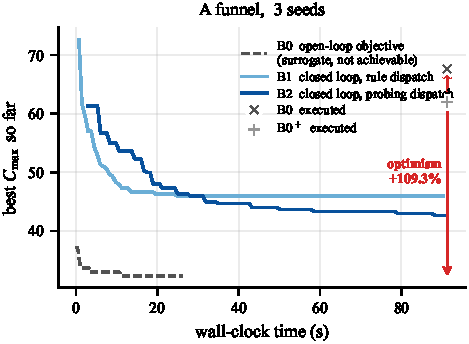
\includegraphics[width=\columnwidth]{fig/fig_convergence_closedloop.pdf}
\Description{Best-so-far makespan against wall-clock time for the ladder
configurations, with the open-loop curve marked as a surrogate objective and its
realizable value shown as a separate point. Each curve carries a shaded band
giving the min-to-max range across the three seeds.}
\caption{Convergence curves on a single \texttt{funnel} instance; the horizontal axis is wall-clock time, the curves are the time-wise mean over seeds,
and the shaded band is the seed-to-seed \emph{range} (this figure has only three seeds, not enough to support quartiles).
The solid lines (B1, B2) are the realized makespan from the first instant; the dashed line is the open loop's own surrogate objective, i.e.\ the quantity it is actually optimizing;
crosses and pluses mark where the same plan sits after conflict-free routing.
The gap between the end of the dashed line and the cross is the optimistic margin of that instance: the open loop does not fail to converge; it converges to a surrogate that cannot be realized.
This figure takes only three instances and three seeds and carries no statistical claim; every statistic in this chapter is taken from the main batch of $\NCases$ instances $\times$ $\NSeeds$ seeds.
The wall-clock budget of this figure is $46.3$ seconds, different from the $90$ seconds of the main batch.}
\label{fig:convergence}
%% From fig/fig_convergence.py -> fig_convergence_closedloop.pdf;
%% ladder_convergence.csv and ladder_cost.csv via tools/ladder_diag.py.
%% Illustrative (shape and gap only); prose statistics always use
%% baseline_ladder.csv.  Three instances x three seeds.
\end{figure}

\paragraph{Reservation-table-aware dispatching.}
Fix the open or closed loop and change only the vehicle-selection rule.
Inside the \emph{closed loop},
$\text{B1}\to\text{B2}$ is $-\GainProbeLoop$ ($p\PProbeLoop$), with pseudomedian \HLProbeLoop{} and
$95\%$ confidence interval \CIProbeLoop{}.
The two levels share the same scheduling search and the same budget; they differ only in whether vehicle selection uses a trial query on the reservation table.
This is an aggregate convention: the interval does not cross zero, and its lower end is less than one percentage point from zero; after a family-wise correction, no instance is significant on its own (the uncorrected count is \CellsSigProbe{} instances), and two of the ten instances have a positive sign---on vehicle-to-arm ratios $1.0$ and $2.0$, B2 is slower than B1 (Table~\ref{tab:main}).
Thus $-\GainProbeLoop$ is an average on this instance family, not a point estimate that can be realized per instance;
Section~\ref{sec:whichcongestion} states this resolution limit.

Under the \emph{open loop}, the same rule is $-\GainProbeOpen$ ($p\PProbeOpen$), likewise significant.
It corresponds to the segment of~\cite{sun2023integrated}'s two-stage structure relative to the open loop of~\cite{li2026framework};
the magnitude (\GainProbeOpen{}) is far smaller than that of the closed loop (\GainLoopRule{}).
Selecting a vehicle from the reservation table is significant under both the open and the closed loop, but much smaller, and by itself it does not explain the $\text{B0}\to\text{B2}$ reduction.

\paragraph{End-to-end.}
$\text{B0}\to\text{B2}$ is $-\GainEndToEnd$ in the aggregate
($p\PEndToEnd$; of the $\NPairs$ pairs, $\WinEndToEnd$ wins, $\LoseEndToEnd$ losses, $1$ tie).
The two paragraphs above have already taken it apart: from open-loop planning with rule-based dispatching to closed-loop planning with reservation-table-aware dispatching, makespan falls by about one fifth.


\subsection{Near-additivity and non-substitutability}
\label{sec:complement}

The three quantities of the previous section have different magnitudes.
Changing only vehicle selection under the open loop: $\GainProbeOpen$, significant but small.
Changing only whether the search includes yielding wait, under rule-based dispatching: $\GainLoopRule$, significant and large.
Changing vehicle selection again inside the closed loop: the aggregate mean is $\GainProbeLoop$, and on the two vehicle-to-arm-ratio instances $1.0$ and $2.0$ B2 is slower than B1, which pulls the mean down.
This section answers two things separately: whether the two can substitute for each other, and whether there is a positive interaction.

\paragraph{Interaction.}
If the closed loop and dispatching were independent of each other, the end-to-end gain would equal the compound of the two separate gains: from the closed loop under rule-based dispatching ($\GainLoopRule$) and dispatching under the open loop ($\GainProbeOpen$) one obtains $\GainIndepProduct$.
The measurement is $\GainEndToEnd$, slightly below that prediction---\emph{no positive interaction is detected}, and the two are near-additive.
They do not amplify each other.

\paragraph{Non-substitutability.}
Changing only vehicle selection under the open loop cannot replace the closed loop.
Fixing the schedule by unimpeded travel times and selecting vehicles only from the reservation table yields about $\GainProbeOpen$; including yielding wait in the search and still using rule-based dispatching yields about $\GainLoopRule$.
The same dispatching rule placed in a two-stage structure of the~\cite{sun2023integrated} kind is useful up to the open-loop dispatching level; to obtain the closed-loop reduction, yielding wait must enter fitness during the search.
B2 is still best end-to-end because it stacks the two gains, not because a positive interaction exists.

\paragraph{Relation to schedule-then-resolve.}
The gap of this route is not in second-stage dispatching---that stage does have a significant gain of $\GainProbeOpen$ under the convention of this paper---but in the first stage not including yielding wait, so the closed-loop quantity cannot enter.
The drop above is a point measured on the instance family of this paper, not a proven bound.

\subsection{Three-factor scans and per-instance resolution}
\label{sec:whichcongestion}

The aggregate comparison of Section~\ref{sec:main} rests on $\NCases$ instances.
This section takes them apart by layout, vehicle-to-arm ratio, and flexibility.
The closed loop can be read as a trend by family; dispatching cannot be resolved on a single instance.
That asymmetry is what this section reports.
Each of the three families corresponds to an expectation that can be stated in advance.

\emph{Layout (Family A)} tests whether the gain grows with contention intensity: both paths handle contention, and with weak contention there is nothing to work on.
\texttt{funnel} and \texttt{high} differ only by one parallel lane at the station, the min-cut halves, and that is the cleanest contrast.

\emph{Vehicle-to-arm ratio (Family B)} tests whether there is a fleet-size upper bound at which the gain is swallowed by overhead.
Trial-query cost grows approximately linearly with the fleet; the pruning of Section~\ref{sec:speedup} has its lowest cut rate on the largest fleet.
The four levels are $N_A/N_M\in\{0.5,1.0,1.5,2.0\}$, of which $1.5$ is the shared base point \texttt{A funnel}.

\emph{Flexibility (Family C)} tests whether the gain depends on room to reassign.
$F\in\{0.3,0.6,1.0\}$, of which $0.6$ is likewise the base point.

\paragraph{Per-instance resolution.}
The significance marks of Table~\ref{tab:bytag} decide which instances may be read by sign.
Testing each of the $\NCases$ instances once, ``at least one significant'' under the global null is far above $5\%$.
Per-instance tests therefore receive a Holm correction by family, the family being the $\NCases$ instances of one effect (the closed loop and dispatching each form a family; pooling the twenty into one family would be correcting a contrast that was never made).
The marks of Table~\ref{tab:bytag} and Figure~\ref{fig:prediction3} are all based on the corrected $p$.

After correction the closed loop remains significant on its own in \CellsSigLoopAdj{} instances (uncorrected \CellsSigLoop{} instances; the largest corrected site is $p\PLoopCellMax$, so the judgement does not depend on whether a correction is applied); the only exception is the tightest-fleet instance ($\text{B0}\to\text{B1}$ is \GainLoopStarve{}, not significant).
The closed loop can therefore be read as a trend by family.
Dispatching inside the closed loop is significant on \CellsSigProbe{} instances before correction (the two ends of Family~C, $p\PProbeFlexLoRaw$ and $p\PProbeFlexHiRaw$), and \emph{on \CellsSigProbeAdj{} instances after correction}: Holm gives $p\PProbeFlexLoHolm$ and $p\PProbeFlexHiHolm$, Benjamini--Hochberg $p\PProbeFlexLoBH$ and $p\PProbeFlexHiBH$, likewise not significant.
No instance can stand on its own.
Its magnitude (a few percentage points) is of the same order as the lower limit that $\NSeeds$ seeds on one instance can resolve; only the $\NPairs$ pairs in the aggregate lift it out of the noise; even in the aggregate it only just clears: the pseudomedian is \HLProbeLoop{}, the $95\%$ interval is \CIProbeLoop{}, it does not cross zero, and its lower end is less than one percentage point from zero.
The per-instance readings of dispatching below are given only as direction, not as a conclusion; a judgement of sign is given only in the aggregate.

\begin{table}[t]
\caption{Per-instance four-level ladder results and the two effects of the closed loop and of dispatching, blocked by the three families (each instance is $n=\NSeeds$ comparisons paired by seed).
Significance marks are given by the \textbf{Holm-corrected} $p$ (two-sided Wilcoxon signed-rank test); the family is the
$\NCases$ instances of one effect: $^{*}p<0.05$, $^{**}p<0.01$; $^{\dagger}$ means significant before correction and not significant after, and the sign of that instance is not taken as a conclusion.
Contention intensity is read off from the instance structure.
A negative value means a lower makespan.
The two gain columns use the same estimator as Table~\ref{tab:main} (the mean of pairwise relative gains over seeds); the mean of the ten instances equals the aggregate of that table within rounding (the digit-wise recomputation uses unrounded values); the column cannot be recovered by dividing the two means in the same row.
\texttt{A funnel} is at once $N_A/N_M=1.5$ of Family~B and $F=0.6$ of Family~C; it is run only once and occupies only one row.}
\label{tab:bytag}
\small
%% Generated by family A/B/C.  Gain column = mean of pairwise relative gains
%% (same estimator as tab_main).  Stars by Holm p; dagger = raw-only.
\input{tab/tab_bytag_EN.tex}
\end{table}

\begin{figure}[t]
\centering
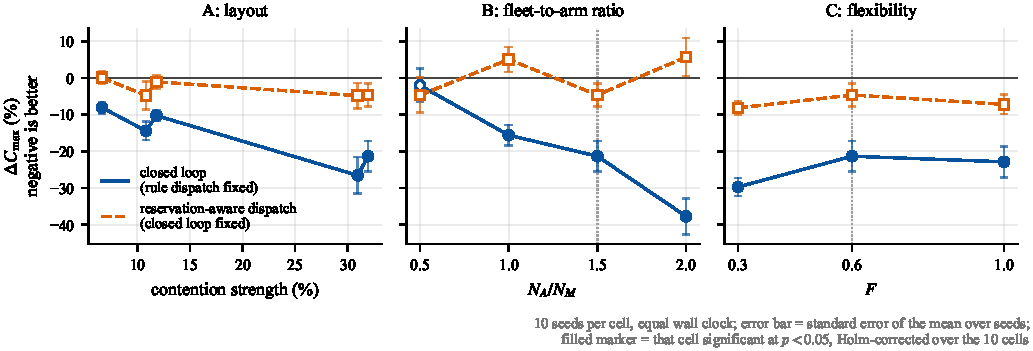
\includegraphics[width=\columnwidth]{fig/fig_prediction3.pdf}
\Description{Three panels of line plots: closed-loop gain and reservation-aware
dispatch gain across layout (vs contention), fleet-to-arm ratio, and flexibility. After
Holm correction over the ten cells the closed-loop curve is filled, hence
significant, at nine of ten cells, while the dispatch curve is hollow at every
cell, and its sign alternates across the four fleet-ratio levels. Error bars
give the standard error of the mean over the ten seeds of each cell; the
dispatch bars cross zero at every cell and the closed-loop bars do not.}
\caption{Distribution of the closed loop and of dispatching on the three families.
Left: Family~A (layout), horizontal axis contention intensity; middle: vehicle-to-arm ratio $N_A/N_M$; right: flexibility.
Families~B and~C include the shared base point ($1.5$ and $0.6$ at the hollow vertical lines), also listed as \texttt{A funnel} in Family~A.
A filled marker remains significant after Holm correction ($p<0.05$, the family being the $\NCases$ instances of one effect); a hollow marker is not significant.
Error bars are the standard error of the mean of pairwise relative gains over the $\NSeeds$ seeds of that instance.
The closed loop is significant on \CellsSigLoopAdj{} instances and rises roughly with contention; after correction dispatching is significant on \emph{no instance}, the error bars cross zero on every instance, and the sign still alternates across the four vehicle-to-arm-ratio levels.
What this figure is to be read for is whether the two curves can be distinguished from zero, not the shape of the dispatching curve.}
\label{fig:prediction3}
%% From fig/fig_prediction3.py and baseline_ladder.csv.
%% x-axis: Family A uses contention intensity; B/C use the factor level in the
%% instance name (written by abc_matrix).  Shared base A funnel has no level in
%% the name; the script fills (1.5, 0.6) from abc_matrix.BASE.
%% Filled/open markers follow Holm p over the ten instances of that effect
%% (not the current panel).  The dispatching curve is all open.
\end{figure}

Table~\ref{tab:bytag} and Figure~\ref{fig:prediction3} give the per-instance results.
The three families are read differently.

\emph{Layout family.}
The closed loop rises roughly with contention intensity and is significant on all five instances: on the least congested \texttt{scatter} (contention \ContentionLo{}) $\text{B0}\to\text{B1}$ is \GainLoopScatter{}; on \texttt{mid}/\texttt{low} it is \GainLoopMid{}/\GainLoopLow{}; on \texttt{funnel}/\texttt{high} it is \GainLoopFunnel{}/\GainLoopHigh{}.
``Roughly'' because there are two inversions, of different kinds.
\texttt{low} has higher contention than \texttt{mid} and a smaller gain; it crosses the topological boundary of Section~\ref{sec:instances} (grid versus dumbbell, farthest trip \LegGrid{} versus \LegDumbbell{}) and is not a pure contention inversion.
\texttt{funnel} has higher contention than \texttt{high} and a smaller gain: both are dumbbells and differ only by one parallel lane at the station, which is the designated cleanest contrast, and \emph{this is the inversion that is a counter-example}.
What can be said is the magnitude---the most congested instance \GainLoopFunnel{} versus the least congested \GainLoopScatter{}, about two and a half times---not a monotone ranking of gain by contention.
Contention intensity compresses congestion into one number and does not separate how much of it can be routed around by reassignment; limitation~(1) of Section~\ref{sec:limitations}.
Dispatching is not significant on any instance of this family; only the direction is recorded: four of the five instances are negative, the same direction as the closed loop.

\emph{Vehicle-to-arm-ratio family.}
It was intended to pin down an applicable upper bound, and it does not.
Dispatching inside the closed loop at the four levels is, in order, $-\GainProbeStarve$ ($N_A/N_M=0.5$), \GainProbeFleetOne{} ($1.0$), \GainProbeFleetBase{} ($1.5$, the base point \texttt{A funnel}), \GainProbeFleetTwo{} ($2.0$): the sign alternates, and none of the four instances is significant ($p\PProbeFleetHalfRaw$, $p\PProbeFleetOneRaw$, $p\PProbeFleetBaseRaw$, $p\PProbeFleetTwoRaw$; these four are the values \emph{before} correction, and they do not even reach the uncorrected threshold).
If only $0.5$, $1.0$, and $2.0$ are taken, the curve looks like the monotone rise predicted by the cost law, and a previous version wrote ``$N_A/N_M\ge 1$ is already an applicable upper bound''; after the middle base point is put back, that narrative does not hold.
When the effect is of the same order as the per-instance noise, \emph{subset selection itself can manufacture a trend}; the way to block it is to complete the scan and test instance by instance.
The upper bound predicted by Section~\ref{sec:costlaw} is therefore still an untested prediction: to test it, the number of seeds would have to be high enough to resolve a few percentage points, beyond the budget of this paper.
The closed loop at $1.0$ and $2.0$ is \GainLoopFleetOne{} and \GainLoopFleetTwo{}, both significant: a larger fleet mainly changes how much the closed loop can reduce, not dispatching.

\emph{Flexibility family.}
It was intended as the only family on which dispatching could support a conclusion, and that claim was withdrawn after Holm correction.
At $F=0.3$, $0.6$, and $1.0$, dispatching is \GainProbeFlexLo{}, \GainProbeFleetBase{}, and \GainProbeFlexHi{}: the three have the same sign, and the two ends are the two largest magnitudes among all $\NCases$ instances (the base point falls back to the level of the rest); the two ends $p\PProbeFlexLoRaw$, $p\PProbeFlexHiRaw$ rise after correction to $p\PProbeFlexLoHolm$, $p\PProbeFlexHiHolm$ and are no longer significant.
This family supplies only directional evidence of the same sign as the aggregate and of the largest magnitude.
Same sign at the three levels, without the sign alternation of the vehicle-to-arm ratio, is compatible with ``corridor contention is handled mainly by vehicle selection and timing, and does not depend strongly on whether another arm remains'': if it were only a bypass of a flexible shop, $F=0.3$ should fail first, and it is precisely the instance of largest magnitude.
Compatibility is not confirmation.
The closed loop is \GainLoopFlexLo{} and \GainLoopFlexHi{}, still significant per instance after correction.

\paragraph{An independent batch of self-generated instances.}
The readings above come from one instance family and one baseline.
A cross-check uses another batch of self-generated instances that still have contention (public benchmarks are in Section~\ref{sec:external}, where contention has been removed): $\MatrixCells$ instances $\times$ $10$ seeds, $\MatrixRuns$ runs in all.
Both the instance core and the baseline differ: the baseline is two-stage surrogate transport, crossed on four contention levels and four heterogeneity levels.
The budget and the seeds differ as well: wall-clock time is calibrated per instance from $30.2$ to $72.9$ seconds (configurations inside the batch share the same calibration, so among configurations it is still an equal budget), and another ten seeds are used.
The \emph{integration gain} (two-stage $\to$ closed-loop) is \GainIntegMatrix{}, significant on \SigIntegMatrix{} of the $\MatrixCells$ instances, ranging from \GainIntegMatrixLo{} to \GainIntegMatrixHi{}, consistent in direction and magnitude with the closed loop of this chapter.
Every count of significant instances cited from this batch is an \emph{uncorrected} count from that batch's own report (the second exception of Section~\ref{sec:protocol}), used only as a check of direction and magnitude, not as a per-instance assertion.

\paragraph{Heterogeneity does not inflate the closed-loop gain.}
The four $H$ levels of that batch answer the question left by Section~\ref{sec:instances}.
Splitting the $\MatrixCells$ instances into four bins by $H$ (four instances per bin, one from each contention level), the integration gain is: \GainIntegHZero{} at $H=0$, \GainIntegHLow{} at $H=0.15$ (measured \MatrixHMeasLow{}), \GainIntegHMid{} at $H=0.3$, \GainIntegHHigh{} at $H=0.5$; the rank correlation of gain with $H$ is a weakly negative \RhoIntegH{}.

The measured $H=\MatrixHMeasLow$ falls near the public-instance median \PubHMed{}, and its \GainIntegHLow{} differs from the \GainIntegHMid{} at $H=0.3$ by less than half a percentage point: setting $H$ above the literature range did not inflate the closed-loop gain.
The expectation that the gain rises with $H$ does not hold---the trend is not monotone, and the rank correlation is negative.
Each bin has only $4$ instances, and the within-bin spread (\GainIntegMatrixLo{} to \GainIntegMatrixHi{}) is far larger than the gap among bins, so this supports only ``the gain does not rise with $H$'' and is not sufficient to assert that $H=0.5$ is lower.
It is compatible with the definition of Section~\ref{sec:features}: as $H$ grows, processing-time differences among optional arms gradually outweigh differences in corridor reachability, and assignment is decided more and more by which arm is fast and less and less by which path is not blocked.
$H=0$ closes the trade-off, not the opportunity: processing times inside $\Omega_{ji}$ are identical, reassignment need not trade processing time for traversal time, and it becomes a pure congestion decision of zero cost; that bin has the highest gain of the four (\GainIntegHZero{}), consistent with the definition.
Thus $H$ makes ``which arm to choose'' a trade-off---without it the reversal of Section~\ref{sec:Chapter_I} cannot be stated---but it is not an amplifier of the closed-loop gain.
The closed-loop gain comes from whether yielding wait is included during the search; how strong the contention is is decided by layout and fleet, not by $H$.

That batch gives reservation-table-aware dispatching \GainProbePre{}, significant on $0$ of the $\MatrixCells$ instances, the opposite direction from $\GainProbeLoop$ of this chapter.
The cause is identified: the batch ran before the two speed-ups of Section~\ref{sec:speedup}, when the overhead of the same rule had not yet been reduced.

\subsection{Ablations and controlled negative controls}
\label{sec:pricing}

Section~\ref{sec:interface} listed three choices for the inter-layer interface.
The default configuration uses only the first (reservation-table-aware dispatching); the other two have both been implemented and measured, and neither has a net gain under an equal wall-clock budget.
This section reports those measurements.

\subsubsection{Yield-record-guided local search}
On the $\MatrixCells$-instance data of Section~\ref{sec:whichcongestion}, turning off yield-record feedback has a relative gain of \GainCertMatrix{} (significant on only $1$ of the $\MatrixCells$ instances), and turning off the staggering operator has \GainStaggerMatrix{} (significant on $2$ instances).
Neither is positive: under an equal wall-clock budget, spending evaluations on this neighbourhood is worse than giving them back to the population cycle.
The mechanism is explained in Section~\ref{sec:whycost}.

These two ablations may cite that earlier batch; the dispatching ablation may not: the yield record and staggering were not changed before or after the two speed-ups, and their cost does not vary with pruning; the cost of dispatching is precisely what the speed-ups target.

\subsubsection{Surcharge on corridor--time slots}
Section~\ref{sec:interface} noted that attaching a further cost to already occupied corridor--time slots counts a second time a delay that fitness has already included.
That argument shows that a surcharge adds no information; it does not give how much worse the makespan becomes.
The two must be measured separately.
$\theta$ is scanned under both budget conventions, and the search width of path planning is held fixed at every $\theta$, so that the surcharge is not mixed with ``how many entry times are examined''.

\begin{figure}[t]
\centering
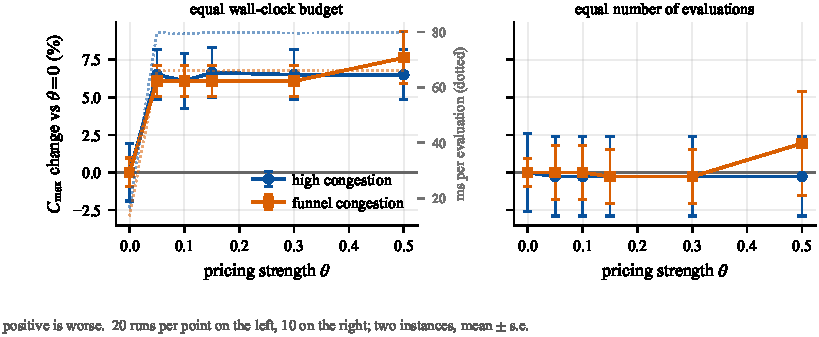
\includegraphics[width=\columnwidth]{fig/fig_theta.pdf}
\Description{Two panels of makespan change relative to theta equals zero against
pricing strength: under equal wall-clock the penalty is large and flat, under
equal evaluations it is absent. Markers are means over seeds and error bars are
the standard error of the mean. The batch is two separately generated instances
that are not members of the paper's A/B/C families.}
\caption{A surcharge on corridor--time slots.
A positive value means worse.
Under equal wall-clock time (left), the makespan worsening appears as soon as the surcharge is turned on, then stays flat over a ten-fold range of $\theta$, in step with the cost per evaluation on the right axis; under an equal number of evaluations (right) the worsening disappears.
The damage comes from a higher cost per evaluation and fewer evaluations inside the same budget, not from the price choosing the wrong path.
Markers are means, error bars are the standard error of the mean, and the number of runs per point is marked in the figure footer; ``significant'' means a two-sided Wilcoxon signed-rank test of each $\theta$ against $\theta=0$, paired by seed.
This figure uses two instances of $8$ jobs $\times\,4$ machines $\times\,4$ vehicles, which do \emph{not} belong to Families A/B/C of Table~\ref{tab:instances} (those are uniformly $12\times 8\times 12$); the legend labels \texttt{high}/\texttt{funnel} are layout tags only, and they are not the same instances as the like-named pair in Family~A.
The left panel has $10$ seeds and the right panel $5$ (a subset of the former); the wall-clock budgets are $48.9$ and $60.7$ seconds, both different from the $90$ seconds of the main batch.
The batch was collected \emph{before} the two speed-ups of Section~\ref{sec:speedup}; the surcharge mechanism was not changed before or after the speed-ups, and its cost is independent of pruning (pruning acts on the dispatching trial query, not on multi-label routing), so the judgement of this section still holds, but it cannot be placed beside the other tables of this chapter instance by instance.}
\label{fig:theta}
%% From fig/fig_theta.py, theta_sweep.csv and theta_sweep_gen.csv
%% (08-05; 2 instances x 10 seeds; left 20 runs/point, right 10).
%% Pre-speed-up batch, contemporaneous with the matrix batch of Section 5.5.
%% Surcharge overhead is independent of pruning (pruning acts on the trial
%% query, not on multi-label routing), so the measurement still holds.
\end{figure}

The measurements are in Figure~\ref{fig:theta}.
Under equal wall-clock time, every $\theta$ tried makes the makespan worse and significantly so, and the worsening is flat over a ten-fold range of $\theta$; under an equal number of evaluations, the same comparison cannot be distinguished from zero.
Routing with the extra cost completes about one fifth as many evaluations inside the same budget as routing without a surcharge: the surcharge does not rank candidates in the wrong order; it lets far fewer of them be evaluated inside the same budget.

Two further points rule out other readings.
First, $\theta$ is not a useful knob on this problem: across two orders of magnitude, priced routing changes the same few paths, pays the same total price, and returns the same makespan; the cumulative price is only a small fraction of total travel time, not enough to overturn the order of arrival times in $\text{arrival time}+\theta\cdot\text{price}$.
Only when $\theta$ is large enough for price to dominate arrival time does the double-counting show, and then makespan worsens sharply.
Second, the overhead is structural, not caused by a nonzero price: the runtime ratio of the same decode with and without a price is the same at every $\theta$---what is paid is ``maintain a Pareto front at every node, try several entry times on every arc'', independently of whether a surcharge is actually applied.
This is what Lemma~\ref{lem:label} says: introducing a second criterion means total-order dominance is no longer available, and a single-label search must be replaced by a multi-label search.

The two budget conventions disagree on magnitude and not on sign.
The part that does not depend on the implementation is this: whether the price comes from a finite difference of corridor capacity or from a critical-chain proxy, what is charged is an occupancy fee whose consequence has already been paid in the yielding vehicle's arrival time.
Whenever fitness is taken from a complete conflict-free decode, yielding wait has already been counted, and a further surcharge is inert; the comparison is then decided by the cost of ``equipping this inert signal with a multi-label search''.
Therefore, before thickening the inter-layer interface, first see whether the receiving layer's objective already contains the quantity the interface would pass; if it already does, that thickening is harmful under the convention of this paper.

%% Demoted from a standalone subsection: mechanism explanation of the ablation,
%% not a first-level finding.
\subsubsection{Dilution and overhead}
\label{sec:whycost}

Why the yield record and staggering fail to offset their overhead can be measured; the same measurement also shows why the overhead of reservation-table-aware dispatching must be reduced first.

\paragraph{Where the extra evaluations are spent.}
Yield-record-guided local search consumes a large share of all evaluations, and of the neighbours it decodes, the fraction that improves makespan is below one in fifty.
The improvements themselves are real; the same evaluations given back to the population cycle produce more.

The low hit rate is not an implementation defect.
The neighbourhood is by construction both small and directed (Section~\ref{sec:ls}); directed and still low-hit means that after reassignment or staggering, the operations named by the record do not shorten the critical chain.
Three repairs were tried: scoring reassignment by expected yield on the path rather than by unimpeded distance, replacing the adjacent swap of staggering by a directed insertion, and accepting a plateau move that leaves makespan unchanged but lowers total yield.
Each was compared independently with the unchanged operator under an equal number of evaluations, and \emph{none} was significant.
The failure is in the signal, not in how the signal is used.

\paragraph{Dilution along the critical chain.}
A yield record names the corridor, the time slot, and the transport that first occupied that corridor for a given yield; that is the information needed to remove \emph{that one} event.
Makespan is attained along a chain; removing one corridor delay usually pushes another constraint tight---an upstream operation, a robotic arm, or another corridor---and the realized improvement is only a fraction of the delay that was removed.
The acceptance rule re-extracts the critical chain after every acceptance for exactly this reason.
When the bottleneck is only one of several bottlenecks of comparable magnitude, feedback that can name the bottleneck does far less than the duration of that yield.

\paragraph{Why dispatching changes sign before and after the speed-ups.}
The dilution of the previous paragraph acts on reservation-table-aware dispatching as well: the trial query selects the vehicle with the earliest delivery of the current task, which is a local improvement; makespan still has to pass through the whole critical chain, and the realized reduction is only a part of that.
After dilution the reduction is still positive, but only a few percentage points.
Before the speed-ups, the cost of a single evaluation is \CostMultBefore{} times that of rule-based dispatching, the number of evaluations inside the same wall-clock time is not enough, and the net effect falls into the noise (the batch of Section~\ref{sec:whichcongestion}).
After Section~\ref{sec:speedup} reduces the cost to \CostMultAfter{} times, that same reduction becomes significant in the aggregate.

Under a fixed budget one has to look at two quantities that can be measured separately and changed separately: how much makespan reduction remains after dilution, and how much extra each evaluation costs.
The two do not fail together.
For yield-record-guided local search the problem is the first: the reduction left after dilution is too small, and the three neighbourhood repairs did not reach significance under an equal number of evaluations.
For dispatching the problem is the second: the post-dilution reduction was already there, and it was not significant at first because the cost per evaluation was too high; that cost can be reduced without changing the selected vehicle or the timetable.
The default configuration therefore keeps dispatching and does not use the yield record to generate the neighbourhood.


\subsection{The cost law and the effect of the two speed-ups}
\label{sec:costlaw}

The cost of a single evaluation and the number of evaluations are two ways of spending the same stretch of wall-clock time.
The same dispatching rule has a net effect that falls into the noise before the speed-ups and is significantly positive after them, so the two themselves are measured.

\paragraph{Two budget conventions.}
Figure~\ref{fig:protocol} gives the cost per evaluation of each configuration, and the number of evaluations actually completed inside the same budget cap.
The cost spans about two orders of magnitude: the cheaper configuration completes more evaluations, and the open loop uses less than two tenths of the wall-clock time to complete the largest number of evaluations.
Comparing at equal generation count gives the more expensive configuration more compute; aligning wall-clock time lets the cheaper configuration evaluate many more times.
Neither convention is presented on its own.

\begin{figure}[t]
\centering
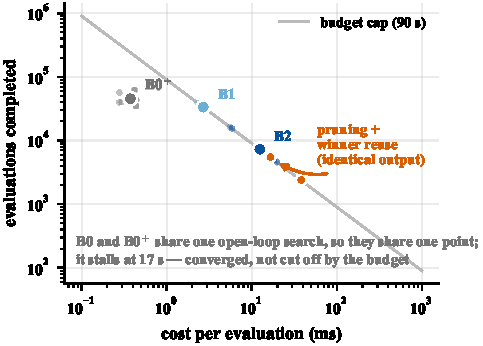
\includegraphics[width=\columnwidth]{fig/fig_protocol.pdf}
\Description{A log-log scatter of cost per evaluation against evaluations
completed. A grey hyperbola marks the 90-second budget cap. The two closed-loop
configurations sit on it, while the open-loop configuration sits well below it
because it stalls after about seventeen seconds. An arrow shows the pruning
ablation moving one configuration along the line without changing its output.}
\caption{A fixed wall-clock budget locks the cost of a single evaluation and the number of evaluations completed onto a hyperbola; the grey line is the $90$-second cap shared by every configuration.
Sitting on the line means cost $\times$ count equals that configuration's wall-clock time.
The two closed-loop configurations sit on the line---every run uses the full budget; the open loop sits \emph{below} the line, because it stops of its own after a little over four hundred generations without improvement, converging in about $17$ seconds, and is not cut off by the budget (Section~\ref{sec:protocol}).
B0 and B0$^+$ share the same open-loop search and therefore share a point; they differ only in how they are executed.
Pale small points are the per-instance readings of three instances; the filled large point is their geometric mean: on a log axis only the geometric mean preserves ``cost $\times$ count $=$ that configuration's wall-clock time''.
The orange arrow is the on/off pair of pruning and winner-path reuse---Proposition~\ref{prop:speedup_equiv} guarantees that one can move along that line \emph{without changing the output}, so this displacement is only a saving of compute.}
\label{fig:protocol}
%% From fig/fig_protocol.py; ladder_cost.csv and prune_ablation.csv.
%% If the latter is missing the script omits the orange arrow.
\end{figure}

Figure~\ref{fig:protocols} runs the same set of comparisons once under each convention.
Equal generation count does not pay for the extra cost per evaluation and therefore favours the configuration whose evaluation is more expensive: reservation-table-aware dispatching relative to rule-based dispatching is \GainProbeSameGen{} ($p\PProbeSameGen$); under equal wall-clock time, before the speed-ups, the same comparison is left at \GainProbeSameClock{} ($p\PProbeSameClock$), almost zero.
Equal generation count asks whether the extra routing step improved the ranking of that generation; equal wall-clock time asks whether makespan fell in the same stretch of time.
Both questions are well posed; one must not be reported as the other.

\begin{figure}[t]
\centering
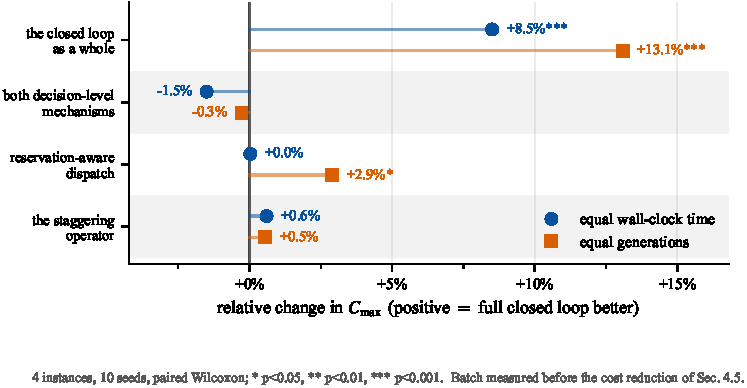
\includegraphics[width=\columnwidth]{fig/fig_protocols.pdf}
\Description{The same paired comparisons shown twice, once under an equal
wall-clock budget and once under an equal number of generations.}
\caption{The same set of comparisons under two budget conventions.
Each row is named by the mechanism it isolates, not by a pair of configurations.
The difference between the two markers comes from the convention: reservation-table-aware dispatching is \GainProbeSameGen{} under equal generation count ($p\PProbeSameGen$) and falls to \GainProbeSameClock{} under equal wall-clock time ($p\PProbeSameClock$), i.e.\ to zero.
The batch ran \emph{before} the two speed-ups of Section~\ref{sec:speedup}, so this row is also the motivation for the control below that moves only the speed-ups.}
\label{fig:protocols}
%% From fig/fig_protocols.py and protocols.csv (4 instances x 10 seeds).
%% Row labels name the isolated mechanism, not the old arm names.
%% Footer states the batch is from before the speed-ups.
\end{figure}

\paragraph{The cost law.}
Reservation-table-aware dispatching raises the routing calls per transport task from $2$ to at most $2N_A$, and the cost grows linearly with fleet size.
The bound used by pruning is tighter when contention is weaker, and more candidates are skipped; the larger the fleet and the stronger the contention, the smaller the cut.
The equivalence self-check of Section~\ref{sec:speedup} gives this direction: of six instances the highest cut rate is on the least congested one (\RouteCallCutHi{}) and the lowest is on the largest fleet (\RouteCallCutLo{})---a decay of effect, not a failure.
The two trends together \emph{predict}: when the fleet is large enough and contention is strong enough, the growth of trial-query cost will catch the gain.
That remains a prediction.
On the four vehicle-to-arm-ratio levels of Section~\ref{sec:whichcongestion} the sign alternates and none of the four instances is significant; that upper bound is not confirmed.
The cost law itself (cost linear in $N_A$, pruning effect falling with $N_A$) is measured directly; the upper bound deduced from it is not.
A previous version treated the former as evidence of the latter; that does not hold.

\paragraph{Turning the two speed-ups on and off.}
The speed-ups and the dispatching rule were introduced one after the other; placing two batches side by side cannot exclude a difference of instance and baseline.
A control that moves only the speed-ups is therefore run: same instances, same seeds, same budget, only pruning and winner-path reuse turned on or off.

Proposition~\ref{prop:speedup_equiv} guarantees that the two optimizations \emph{do not change the output}.
On each of six instances six random chromosomes are taken; the makespans and the dispatch sequences of the two settings are \emph{identical bit for bit}, $36$ groups with no exception; routing calls fall by \RouteCallCut{} in the aggregate.
The output already being the same, turning the optimizations off only makes a single evaluation slower, and the makespan difference under equal wall-clock time comes \emph{only} from the compute that was saved.

Table~\ref{tab:prune}: off$\to$on reduces makespan by a further \GainPrune{} (\WinPrune{} wins / \LosePrune{} losses, $p\PPrune$), the number of evaluations inside the same budget is \EvalRatioPrune{} times, and a single evaluation is sped up by \SpeedupProbe{}.
This joins the two batches: the same rule is \GainProbePre{} on the pre-speed-up matrix batch (significant on $0$ of the $\MatrixCells$ instances) and significantly positive on the post-speed-up ladder batch; the step in between did not change any selection.

\begin{table}[t]
\caption{Changing only pruning and winner-path reuse.
``Off''/``on'' means whether the two are enabled; the bold header is the setting adopted in this paper.
The two settings produce bit-identical output (already passed the equivalence self-check), so the difference comes only from the compute that was saved.
Same instances, same seeds, same wall-clock time; $n=60$ pairs, two-sided Wilcoxon signed-rank test ($^{***}p<0.001$); the aggregate row lists wins/losses/ties and $p$.
Both ratio columns have the \emph{off} setting as denominator, in opposite directions: evaluations as on/off, time per evaluation as off/on.}
\label{tab:prune}
\small
%% Regenerated from prune_ablation.csv by gen_tables_ladder.py.
%% 由 tab/gen_tables_ladder.py 生成,请勿手工编辑
%% 数据源:clbs/output/baseline_ladder.csv 等,见脚本首部
\begin{tabular}{@{}lrrrrrr@{}}
\toprule
& & \multicolumn{2}{c}{$C_{\max}$ (time units)} & & Eval.\ count ratio & Speedup per eval. \\
\cmidrule(lr){3-4}
Instance & Contention & Off & \textbf{On} & $\Delta C_{\max}$ & (on/off) & (off/on) \\
\midrule
A funnel & 31.9\% & 44.80 & 42.10 & $-6.03\%$ & 2.21$\times$ & 2.23$\times$ \\
A high & 30.9\% & 41.60 & 37.70 & $-9.37\%$ & 2.40$\times$ & 2.41$\times$ \\
A low & 11.8\% & 60.50 & 57.00 & $-5.79\%$ & 2.79$\times$ & 2.81$\times$ \\
B NA/NM 0.5 & 15.8\% & 66.70 & 65.10 & $-2.40\%$ & 2.11$\times$ & 2.11$\times$ \\
B NA/NM 1.0 & 30.2\% & 51.90 & 48.90 & $-5.78\%$ & 2.31$\times$ & 2.31$\times$ \\
B NA/NM 2.0 & 32.4\% & 44.50 & 42.20 & $-5.17\%$ & 1.98$\times$ & 2.01$\times$ \\
\midrule
\emph{Pooled} (60 pairs) & --- & --- & --- & $-5.60\%^{***}$ & \multicolumn{2}{r}{50/0/10,\ $<10^{-4}$} \\
\midrule
\multicolumn{7}{@{}l@{}}{\footnotesize HL pseudomedian and $95\%$ CI:$-4.72$ $[-6.34,-3.55]$\,\%} \\
\bottomrule
\end{tabular}

\end{table}

\subsection{Case study: Gantt chart and critical chain on the funnel instance}
\label{sec:casestudy}

Aggregate numbers do not show what happens inside one solve.
This section places B0 and B2 side by side on a single funnel instance and colours the links of the critical chain by Table~\ref{tab:attrib}.

Figure~\ref{fig:case_gantt} draws robotic arms and vehicles on a shared time axis; vehicle rows distinguish empty and loaded legs, and yielding wait is coloured separately.
Three things can be read directly.
In the open-loop solution, yielding wait appears in stretches on the corridors near the station and concentrates on a few vehicles.
The closed-loop solution cuts those waits substantially, and several operations are assigned to an arm that is not the fastest.
The closed-loop solution also balances vehicle idle and busy time more evenly---that is a consequence of the first two points, not a third mechanism: the solution contains assignments of the \eqref{eq:reassign} kind that trade a longer processing time for a shorter, easier path.

\begin{figure*}[t]
\centering
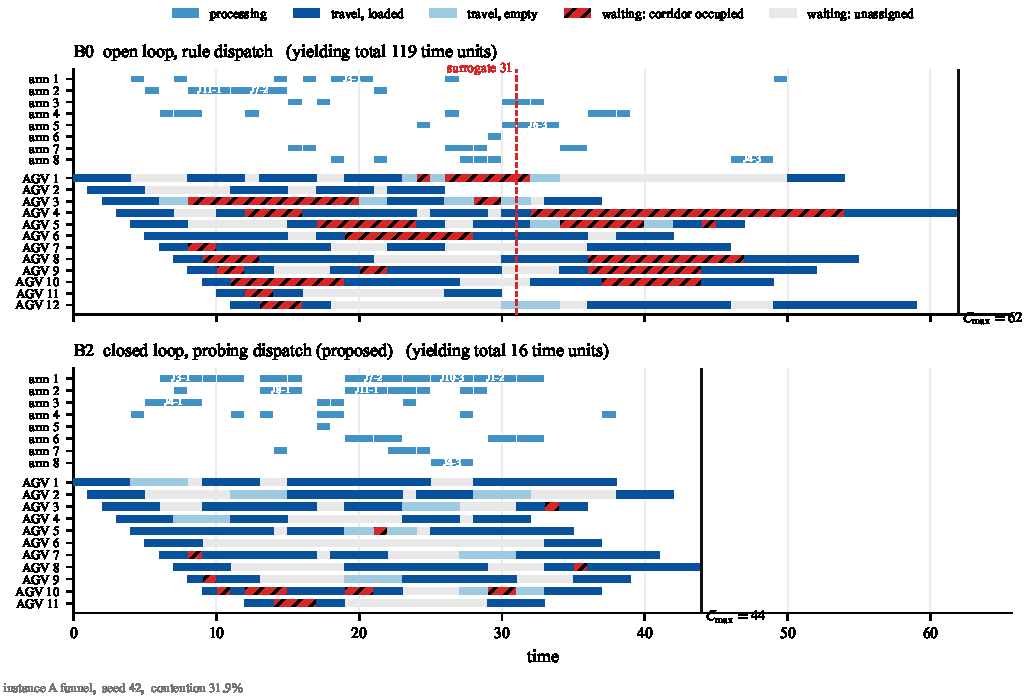
\includegraphics[width=\textwidth]{fig/fig_case_gantt.pdf}
\Description{Side-by-side Gantt charts of the open-loop and closed-loop
solutions on one funnel instance, with arms and vehicles on a shared time axis
and yielding waits shaded separately.}
\caption{B0 (top) and B2 (bottom) on the same funnel instance.
Robotic arms and vehicles share the time axis; vehicle rows distinguish empty and loaded legs, and two kinds of gap.
A gap between the two legs of the same transport task: the vehicle is held at a berth by an occupied corridor, i.e.\ yielding wait, the delay this paper treats.
A gap between different tasks: the vehicle has nothing to do.
The two are coloured separately, so that idle time is not read as yielding wait.}
\label{fig:case_gantt}
%% From fig/fig_case_gantt.py and case_study/*.json (ladder_diag.py --case-study).
%% Yield vs idle is inferred from adjacent task fields, not a stored label.
\end{figure*}

Figure~\ref{fig:case_chain} colours each link by the five labels of Table~\ref{tab:attrib}.
On B0's chain \texttt{corridor} occupies a substantial share; on B2 they largely disappear, and what comes to the top is \texttt{machine} and \texttt{upstream}.
This is the dilution of Section~\ref{sec:whycost}: remove one corridor delay, and another constraint becomes tight.

\begin{figure}[t]
\centering
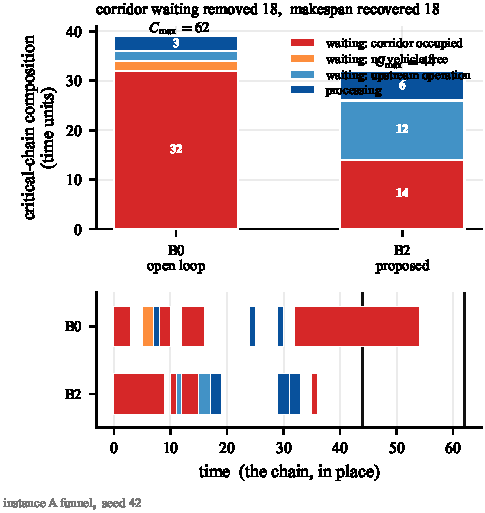
\includegraphics[width=\columnwidth]{fig/fig_case_chain.pdf}
\Description{The critical chain of the open-loop and closed-loop solutions,
with each link coloured by its attribution label.}
\caption{Links of the critical chain coloured by Table~\ref{tab:attrib}.
Top: composition of the two critical chains; the title places ``corridor wait removed'' beside ``makespan actually recovered'', and the difference is the part absorbed by the constraint that came to the top.
Bottom: the same chain in place on the time axis, showing that the bars above are the decomposition of one chain, not a histogram of unrelated events.
In the closed-loop solution \texttt{corridor} largely disappears, and what comes to the top is the arm and the upstream operation.}
\label{fig:case_chain}
%% From fig/fig_case_chain.py and the same case_study/*.json.
%% Labels from decoder.critical_chain(); five classes, none merged into other.
\end{figure}

\subsection{Degenerate comparison on public benchmarks}
\label{sec:external}

The preceding sections compared different configurations of the same codebase on self-generated instances, which excludes implementation differences among configurations but cannot calibrate the absolute level of this implementation: if the upper-level search is weak, the differences among configurations remain credible, while the absolute makespan only reflects the implementation.
This section calibrates the upper-level search on public benchmarks.

\paragraph{What is compared.}
After the exclusivity constraint~\eqref{eq:excl} is removed, the model of this paper degenerates exactly to standard FJSP\_PT (Section~\ref{sec:Chapter_III}), the \emph{same mathematical problem} as the public benchmarks.
$\delta_{\mathrm{ret}}=0$ is additionally taken to align the makespan definition of this batch; it is already a model parameter (Table~\ref{tab:notation}), not the removal of a further constraint.
After the degeneration there is no corridor contention, neither mechanism enters, and what is tested is the \emph{upper-level search}, not the framework of this paper.
The results are reported in a table separate from the self-generated instances, so that the two conclusions do not share one table.

\paragraph{Instances and protocol.}
The \PubNInst{} instances compiled by Homayouni and Fontes~\cite{homayouni2021production} are taken (originating in Fattahi et al.~\cite{fattahi2007mathematical}, $2$--$12$ jobs, $4$--$48$ operations, $2$--$8$ machines), with two vehicles as in the literature~\cite{lim2023twophase} and no return of finished goods.
Travel times are used \emph{as published}, without a shortest-path synthesis: Section~\ref{sec:instances} already noted that \PubNLayoutBad{} of the matrices are not the shortest-path closure of any graph, and a synthesis would change the instance.
After degeneration the road network $G$ enters the model only through $t^{*}$, so the published matrix can be taken directly as $t^{*}$, and a $G$ consistent with it need not exist.
Contention needs $G$ itself, which this batch does not have, so it can be used \emph{only} in the degenerate setting.
Two instances were checked by hand, bit for bit: the published optimum $70$ of $\mathrm{SFJST}01$ equals the station-to-machine trip $4$ plus the two operations $45+21$; the $223$ of $\mathrm{SFJST}03$ equals a tight packing of three operations on one machine.
Neither includes a return; if a return were counted, the former would be $78$.
Reference values: \PubNOpt{} instances have a MILP-proven optimum~\cite{homayouni2021production}; the remaining $4$ take the published best-known~\cite{lim2023twophase}.

\paragraph{Results.}
Table~\ref{tab:external} is \PubNInst{} instances $\times$ \NSeeds{} seeds.
All $200$ runs pass three checks: no solution below the composite lower bound, no validation failure; on the \PubNOpt{} instances with a proven optimum ($160$ runs), no run falls below that value.
The degenerate setting and the literature are the same problem, and a proven optimum is a hard lower bound: falling below it would be an error of conversion or convention, not a better result.
On $\PubNMatch{}/\PubNInst{}$ instances the best solution is \emph{identical bit for bit} to the reference, including all $10$ small instances (\textsc{sfjst}01--10); the mean gap over the \PubNInst{} instances is \PubGapMean{} (median \PubGapMed{}).
The gap rises with size, but not monotonically instance by instance: \textsc{mfjst}03 and \textsc{mfjst}06 both beat their respective smaller neighbours.
The four largest instances ($32$--$48$ operations) have mean \PubGapBig{}, worst \PubGapMax{}; none of the $16$ instances with at most $24$ operations exceeds $5.45\%$.

\begin{table}[t]
\caption{Degenerate comparison on public benchmarks (exclusivity constraint removed; the same problem as the literature).
In the ``reference'' column,
\textsc{opt} is a MILP-proven optimum and \textsc{bk} is a published best-known; the gap is computed from the best
solution over \NSeeds{} seeds.
An asterisk marks instances whose best solution is identical bit for bit to the reference.
Data: \texttt{experiments\_database/gap\_ideal.csv}.}
\label{tab:external}
\centering
\small
\input{tab/tab_external_EN.tex}
\end{table}
%% tab_external() from gap_ideal.csv; the Ops column is counted from
%% hf/*.json (len(proc_time)), not typed.  The same function prints the \Pub*
%% macros.  Edit the CSV, then re-run the script.

\paragraph{The gap is search capability, not an insufficient budget.}
Of the literature's \PubNOpt{} proven optima, the MILP on the largest instance took nearly ten hours (\textsc{mfjst}06, $34\,796$ seconds); each run of this paper uses a few seconds.
The budget is therefore raised by one step (generation cap five times, early-stop threshold $3.3$ times, measured wall-clock time to \PubBudgetRatio{} times) and re-run on the $10$ \textsc{mfjst} instances in the last ten rows of Table~\ref{tab:external}---the gap concentrates there.
The mean gap of these ten falls from \PubGapLoBudget{} to \PubGapHiBudget{} (the base contains only these ten, a different convention from the \PubGapMean{} over the \PubNInst{} instances above), i.e.\ \PubBudgetRatio{} times the compute buys only $\PubBudgetGainPP$ percentage points; \PubBudgetNoGain{} of them fall not at all, and the largest falls from $12.93\%$ to $12.85\%$.
Under both budgets, none of the $300$ runs \emph{hits} the generation cap; all are early-stop convergences, and raising the budget did not make the search run longer.
The gap is therefore mainly the capability boundary of the upper-level search.
Narrowing it on large instances is item~(3) of Section~\ref{sec:future_work}.

\paragraph{Where the gap between the composite lower bound and the best solution comes from.}
Between the composite lower bound and the best solution obtained, the median gap is \LBGapMed{}.
That number is the sum of two stretches: how much the bound lies below the true optimum, plus how much the search solution lies above the true optimum.
On the self-generated instances the optimum is unknown, and the two stretches cannot be taken apart.
On the public instances they can.
Only the \PubNOpt{} instances with a proven optimum are taken: the reference of the other $4$ is a published best-known, the true optimum can only be smaller, and using it as a denominator would overstate ``how much the bound lies below the optimum''.
On these \PubNOpt{} instances, the same composite lower bound lies a median \PubLBSlack{} below the proven optimum and a median \PubLBTotal{} below the best solution of this paper; taking the difference instance by instance, the search solution lies a median $\PubLBResidMed$ percentage points above the optimum (most instances already hit the optimum), and at most $\PubLBResidMax$ percentage points.
Thus on this \emph{contention-free} batch, almost all of the gap between the bound and the best solution is the bound not sitting tight on the optimum, not the search failing to find the optimum.
The self-generated instances cannot inherit this proportion.
The construction of the composite lower bound does not contain corridor contention; the true optimum of a self-generated instance can only be higher or equal because of contention, while the bound stays the same, so the distance from the bound to the true optimum cannot be smaller than on the public instances.
What can be determined is only this: the \LBGapMed{} on the self-generated instances \emph{must not} be read as ``the search is this far short''---the same bound already lies \PubLBSlack{} below the optimum when there is no contention.
How far the search itself sits from the optimum remains unknown on the self-generated instances, so limitation~(3) of Section~\ref{sec:limitations} makes no quantitative assertion about that distance.



\section{Conclusion}

This paper treats a scheduling problem in which flexible assignment and conflict-free AGV routing must be decided together: travel time is produced by routing, and once the corridor to a fast arm is congested, a slower arm that is easier to reach may be the better assignment.
Existing methods either schedule on a constant matrix, or freeze the assignment first and then resolve conflicts, so yielding wait cannot enter every candidate that the search compares.
Against this gap, the bilevel framework connects the two levels along an evaluation path and a decision path, and measures them separately under the same wall-clock budget: the fitness of each candidate is taken from the makespan after conflict-free routing, and a vehicle is chosen by a trial query on the reservation table rather than by unimpeded travel time.
One conflict-free evaluation is about an order of magnitude more expensive than a lookup of the unimpeded matrix, and each extra layer of information returned costs many evaluations; it is therefore also necessary to answer how dispatching can press down the cost per evaluation without changing the selected vehicle or the timetable, and whether, beyond these two paths, thickening the interface---a surcharge on occupied corridor--time slots, or reassignment and staggering from the yield record---can reduce makespan further under the same budget.


\subsection{Findings and contributions}
\label{sec:contributions}

\textbf{(1) The reassignment trade-off when flexibility, heterogeneous efficiency, and corridor contention are present at once.}
Travel time is produced by the routing decision, not read from a constant matrix.
When machine flexibility, heterogeneous processing efficiency, and corridor contention are present at once, and the schedule is optimized for the makespan after yielding wait is counted, if the corridor to a fast arm is congested, a slower arm with better connectivity may be the better assignment.
This paper adopts the problem class of~\cite{vanos2026exact}; the contribution is the solver, not the problem definition; and it supplements a controllable characterization of contention intensity, used to examine how high contention must be before counting yielding wait in the schedule yields a gain.

\textbf{(2) A closed-loop bilevel framework, and the contribution of routing-in-the-loop evaluation to makespan.}
The upper level searches assignment and sequencing by a memetic algorithm; the lower level does conflict-free routing by time-window reservation.
The fitness of each candidate is taken from the makespan after the lower level has completed every transport; what the search compares is not a surrogate that excludes yielding wait.
Proposition~\ref{prop:decodable} and Lemma~\ref{lem:label} guarantee that every chromosome is decodable, that the evaluation is consistent with the conflict model of Section~\ref{sec:Chapter_III}, and that no repair operator is needed.
Relative to the open loop, the closed loop reduces makespan by $\GainLoopRule$ under rule-based dispatching ($p\PLoopRule$), and by $\GainLoopProbe$ under reservation-table-aware dispatching ($p\PLoopProbe$).

\textbf{(3) Reservation-table-aware vehicle dispatching, and two speed-ups that do not change the output.}
Before a vehicle is chosen, a two-leg trial query is run on the reservation table, and the earliest feasible delivery replaces the unimpeded-shortest-path estimate.
Within the closed loop the further reduction is $\GainProbeLoop$ ($p\PProbeLoop$).
The rule raises the cost per evaluation to \CostMultBefore{} times that of rule-based dispatching, enough under the same wall-clock to eat its own gain.
Admissible lower-bound pruning and winner-path reuse do not change the selected vehicle or the timetable (Proposition~\ref{prop:speedup_equiv}; a bitwise self-check on six instances); router calls fall by \RouteCallCut{}, and the cost multiple is pressed to \CostMultAfter{}.
It is significant in the aggregate, but the sample is not sufficient to identify on which class of instances this gain is stable; see limitation~(2) of Section~\ref{sec:limitations}.
Before the speed-ups the same rule fell into the noise, because of the overhead, not because the gain was zero.

\textbf{(4) The closed loop and dispatching differ in the size of their contributions, and dispatching is not yet sufficient to identify on which class of instances the gain is stable.}
The closed loop remains significant on its own after Holm correction on \CellsSigLoopAdj{} of the $\NCases$ instances.
Reservation-table-aware dispatching is significant in the aggregate under both the open loop and the closed loop ($\GainProbeOpen$, $p\PProbeOpen$; $\GainProbeLoop$, $p\PProbeLoop$, $95\%$ interval \CIProbeLoop{}), and after correction is significant on none of the instances on its own, so one knows only that the mean is positive, not on which class of instances it is stably realized.
The end-to-end $\GainEndToEnd$ is close to the independent composite $\GainIndepProduct$ (near-additivity, no positive interaction detected); changing only vehicle selection under the open loop is far from a substitute for the closed loop.
``Schedule first, resolve conflicts later'' resolves conflicts and selects vehicles only in the second stage, and can obtain the open-loop dispatching $\GainProbeOpen$; the first-stage search still ignores yielding wait, so the reduction that corresponds to closed-loop evaluation ($\GainLoopRule$) does not appear.
The numbers above depend on two comparison rules, and the two rules themselves are not a contribution: the four-level ladder changes only one factor at a time, so a gain can be attributed to the closed loop or to dispatching; every configuration is executed by the same conflict-free path planner and rechecked by the same validator, so what is compared is the realized makespan.


\subsection{Limitations}
\label{sec:limitations}

\textbf{(1) The scope of the instance families, and why they had to be self-generated.}
The main experiment fixes the size and only changes structure (Section~\ref{sec:features}), so this paper makes no claim about how the mechanisms vary with size.
Heterogeneity $H$ is fixed at $0.3$; the scan of four $H$ levels comes from that smaller independent batch of Section~\ref{sec:whichcongestion}, so ``the gain does not rise with $H$'' is obtained at \emph{that} size.
The layout family is spliced from two topologies: the three dumbbell levels move only network capacity; the two grid levels switch to a grid and a staggered grid, and topology and distance change together (the farthest leg rises from \LegDumbbell{} to \LegGrid{}, Section~\ref{sec:instances}).
The contention intensity that characterizes the family is again only a one-dimensional summary, and does not distinguish how much of the yielding wait can be bypassed by reassignment.
These two points mean that only the differences among the three dumbbell levels can be cleanly attributed to capacity; the five levels should not be joined into one curve by contention intensity, and they are also two possible reasons why the gain and contention intensity are not strictly in the same order.
They had to be self-generated because this strand still has no usable public benchmark: the usual FJSP\_PT release is a constant matrix, and of the family actually used, \PubNLayoutAsym{}/\PubNLayout{} matrices are asymmetric and \PubNLayoutBad{} are not even a shortest-path closure, so contention cannot be defined (Section~\ref{sec:instances}); the two pieces of work with an explicit road network cannot be compared directly because the reservation unit differs (Section~\ref{sec:fjsppt}).

\textbf{(2) The makespan gain from dispatching is positive on average, but the sample is not sufficient to identify on which class of instances it is stable.}
$\NSeeds$ seeds per instance are enough to resolve the closed loop ($\CellsSigLoopAdj/\NCases$ instances significant on their own after Holm correction).
The magnitude of reservation-table-aware dispatching is only a few percentage points, of the same order as the dispersion among seeds: $\CellsSigProbe/\NCases$ instances are significant before correction and $\CellsSigProbeAdj/\NCases$ after, so the gain is confirmed as positive in the aggregate of $\NPairs$ pairs ($95\%$ interval \CIProbeLoop{}, the lower end less than one percentage point from zero), but the sample is not sufficient to identify on which class of instances it is stable.
Raising the number of seeds by about an order of magnitude is what would be needed to tell on which class of instances it appears, and to test the fleet-size upper bound predicted by the cost law of Section~\ref{sec:costlaw}.

\textbf{(3) The upper-level search has been calibrated on contention-free public benchmarks; with corridor contention, how far the solution sits above the optimum cannot yet be judged.}
The configurations share one code base and report differences among levels; the strength of the upper-level search is common to every level and cannot produce the differences among levels.
The degenerate comparison of Section~\ref{sec:external} is bitwise identical to the literature on $\PubNMatch{}/\PubNInst{}$ instances, and all $10$ small instances hit a proven optimum.
The gap rises with size: the four largest instances average \PubGapBig{}, and raising compute to \PubBudgetRatio{} times buys only $\PubBudgetGainPP$ percentage points, so it is a capability boundary, not a short budget.
On the \PubNOpt{} public instances with a proven optimum, the search shortfall is at most $\PubLBResidMax$ percentage points, and almost all of the gap comes from slack in the bound.
On the self-generated instances the composite lower bound contains no contention, and the median gap to the best solution is \LBGapMed{}, which must not be read as a search gap; this paper also makes no quantitative claim about that distance.
The public instances have no corridor contention, and the lower-level routing and the reservation table still have no proven optimum to compare against.
A smaller effect of a few percentage points (such as \GainProbeLoop{}) is of the same order as the distance of the implementation from the optimum (see limitation~(2)).

\textbf{(4) The surcharge and yield-record-guided local search did not reduce makespan further; if their evaluation cost is pressed down on its own, they must be remeasured.}
Both were judged in the same code base and under the same wall-clock budget.
What was measured is the exchange of cost per evaluation against the number of evaluations: speeding everything up by a constant factor leaves the exchange rate unchanged, and the sign unchanged.
Only pressing down the cost of one interface on its own would change the sign---the dispatching speed-ups of Section~\ref{sec:speedup} are one case already done.
Therefore, if neighbourhood evaluation is changed to re-solve only the perturbed part, it must be measured again (item~(4) of Section~\ref{sec:future_work}).

\textbf{(5) Dynamic accidents such as robotic-arm and vehicle failures are not considered.}
Assumption A7 has already placed robotic-arm and vehicle failures and dynamic job arrivals outside the model.
The ratios reported are limited to the static setting in which the job set and the processing times are known over the planning horizon and equipment does not fail.
When a failure or an online arrival occurs, the value of a mechanism also includes the speed at which it repairs the schedule, not only the quality with which it constructs one; this paper does not measure that dimension (item~(5) of Section~\ref{sec:future_work}).

\subsection{Future work}
\label{sec:future_work}

\textbf{(1) Remeasure on a larger explicit road network, and separate contention from chain substitutability.}
This corresponds to limitation~(1).
The main experiment fixes the size, so the first step is to remeasure on a larger explicit corridor network whether the closed loop and dispatching remain of the same magnitude.
On the layout, split ``whether congestion can be bypassed by reassignment'' and ``whether the critical chain has only one dominant bottleneck'' into two factors; the funnel share $\varphi$ failed to separate the two families it was meant to separate (Section~\ref{sec:features}), and an indicator that has first been checked on instances whose answer is known is needed.

\textbf{(2) Raise the number of seeds, and identify on which class of instances the dispatching gain is stable.}
This corresponds to limitation~(2).
That the makespan gain from dispatching is positive on average has already been confirmed.
Raising the number of seeds by about an order of magnitude, and taking denser levels of the vehicle-to-arm ratio, is what would identify on which class of instances this gain is stable, and would test the cost law: whether there is a fleet size beyond which the growth of trial-query cost catches the gain.

\textbf{(3) On instances with corridor contention, measure how far the solution sits above the optimum.}
This corresponds to limitation~(3).
The \PubGapBig{} on the large public instances is insensitive to a longer time; the seed-to-seed standard deviation of the four instances reaches \PubCvBig{} of the mean, and all are early stops, so what needs to change is the encoding or the neighbourhood.
At the small-size end, exact solutions by logic-based Benders decomposition~\cite{vanos2026exact} are what would separate, when there is corridor contention, how much is slack in the bound and how much is the search not finding the optimum, and would show whether the surcharge and yield-record-guided local search still fail to reduce makespan when the search is stronger.
This does not change the differences among levels, but may thereby also identify on which class of instances the dispatching gain is stable (limitation~(2)).

\textbf{(4) Press the cost down by incremental evaluation, then remeasure yield-record-guided local search.}
This corresponds to limitation~(4).
The decoder state flows forward; when only the part of the sequence after a given position is perturbed, the events and reservations before that stay the same.
Re-solving only the perturbed part is equivalent to pressing down the cost per evaluation of this kind of local search on its own, and then measuring once more under the same wall-clock.

\textbf{(5) Measure the speed of repairing the schedule under robotic-arm and vehicle failures.}
This corresponds to limitation~(5).
Work on the dynamic flexible job shop has already brought machine failures, urgent insertions, and job arrivals into rescheduling~\cite{gui2023dynamic,xiong2024dynamic,dauzereperes2024fjsp}.
The value of a mechanism then also includes the speed of repairing the schedule, not only the time and quality of constructing one.
Which is the better bargain, an evaluator that must re-solve from scratch or one that only changes a local neighbourhood, cannot be carried over directly from the ratios of the static setting.


%\section*{Acknowledgments}
%This work was supported partly by Key Laboratory of Computer Network and Information Integration (Southeast University) of Ministry of Education of China under Grants NO. 93K-9 and Jiangsu Provincial Key Laboratory of Network and Information Security under Grants No.BM2003201.

%%
%% The next two lines define the bibliography style to be used, and
%% the bibliography file.
\bibliographystyle{ACM-Reference-Format}
\bibliography{reference-base}


%% No appendix.  An empty \appendix leaves a blank TOC/header entry in acmart.

\end{document}
\endinput
%%

